% !TeX spellcheck = en_US
%%
%% Text of diploma thesis
%%
%% Tomáš Zítka
%%
\documentclass{book}
\usepackage[english]{babel} 
\usepackage{a4wide}
\usepackage{graphicx}
\usepackage{caption}
\usepackage{subcaption}
\usepackage[utf8]{inputenc}
\usepackage{enumerate}
\usepackage{amssymb, amsmath}
\usepackage{amsthm}
\usepackage{natbib}
\usepackage{ae}
\usepackage{pifont}
\usepackage[all]{xy}
\usepackage{thmtools}
\renewcommand{\listtheoremname}{List of Examples}

% colors
\usepackage[usenames,dvipsnames]{xcolor}
\definecolor{deepblue}{rgb}{0, 0, 0.5}
\definecolor{deepred}{rgb}{0.6, 0, 0}
\definecolor{deepgreen}{rgb}{0, 0.5, 0}
\usepackage{tikz}

% links style
\usepackage[unicode]{hyperref}
\hypersetup{
	colorlinks,
	linkcolor={red!50!black},
	citecolor={blue!50!black},
	urlcolor={blue!80!black}
}
\usepackage{cleveref}

% acronyms
%\usepackage[acronym, xindy]{glossaries}
%\makenoidxglossaries
%\input{./texts/zkratky}

% code typeseting
\usepackage{listings}
\lstset{numbers=none,
		stepnumber=2,
		numbersep=5pt,
		numbers=none,
		tabsize=4,	
		frame=lines,
		language=Python,
		otherkeywords={self},
		breaklines=true,
		breakatwhitespace=true,
		basicstyle=\ttfamily,%\footnotesize
		keywordstyle=\bfseries\color{deepblue},
		commentstyle=\small\color{gray},
		stringstyle=\color{deepgreen},
		showstringspaces=false
}

\lstset{escapeinside={/*!}{!*/}}

\newcounter{lstannotation}
\setcounter{lstannotation}{0}
\renewcommand{\thelstannotation}{\ding{\number\numexpr181+\arabic{lstannotation}}}
\newcommand{\annotation}[1]{\refstepcounter{lstannotation}\label{#1}\thelstannotation}
\newcommand{\lann}[1]{\refstepcounter{lstannotation}\label{#1}\thelstannotation}

%inline code typesseting
\newcommand{\shellcmd}[1]{\texttt{#1}}
\newcommand{\pysauce}[1]{\lstinline!#1!}

% some logos 
\providecommand{\Microsoft}{{\sffamily Microsoft}}	
\providecommand{\Windows}{{\sffamily Windows}}	

%TO-DOcomand
\providecommand{\todo}{\textbf{TODO }}


% math stuff
\newtheorem{theorem}{Theorem}
\newtheorem{princ}{Principle}
\newtheorem{axiom}{Axiom}[chapter]
\newtheorem{claim}{Proposition}
\newtheorem{Lemma}{Lemma}

\theoremstyle{definition}
\newtheorem{definition}{Definition}
\newtheorem{example}{Example}

%\renewcommand{\listtheoremname}{List of examples}

\providecommand{\bracesanddots}[4]{$\langle$#1$\rangle$:$\langle$#2$\rangle$:$\langle$#3$\rangle$:$\langle$#4$\rangle$}
\providecommand{\anglebracs}[1]{$\langle$#1$\rangle$}
\providecommand{\manglebracs}[1]{\langle#1\rangle}
\providecommand{\norm}[1]{\left\lVert#1\right\rVert}
\providecommand{\abs}[1]{\left\lvert#1\right\rvert}
\providecommand{\doteq}{\,\dot = \,}
\newcommand{\pdiff}[2]{\frac{\partial#1}{\partial#2}}
\newcommand{\fdiff}[2]{\frac{\text{d}#1}{\text{d}#2}}
\newcommand{\Laplace}{\Delta}
\newcommand{\DAlambert}{\mathop{}\!\mathbin\Box}

% number classes
\providecommand{\realc}{\mathbb{R}}
\providecommand{\naturc}{\mathbb{N}}
\providecommand{\finaturc}{\mathbb{FN}}
\providecommand{\fisnaturc}{\mathbb{F^*N}}
\providecommand{\comc}{\mathbb{C}}

% convenient math functions
\newcommand\tg{\qopname\relax o{tg}}
\newcommand\tgh{\qopname\relax o{tgh}}
\newcommand\sign{\qopname\relax o{sign}}
\newcommand\cotg{\qopname\relax o{cotg}}
\newcommand\atg{\qopname\relax o{arctg}}
\newcommand\im{\qopname\relax o{Im}}
\newcommand\re{\qopname\relax o{Re}}

\newcommand{\Cls}{\mathrm{Cls}}
\newcommand{\Set}{\mathrm{Set}}
\newcommand{\Fin}{\mathrm{Fin}}
\newcommand{\Nat}{\mathrm{Nat}}

\newcommand{\dom}{\mathrm{dom}}
\newcommand{\rng}{\mathrm{rng}}


\numberwithin{equation}{section}
\usepackage{chngcntr}
\counterwithout{figure}{chapter}
\numberwithin{table}{section}



\title{Discontinuous Galerkin method, its analysis and implementation into SfePy package}
\author{Tomáš Zítka}
%\university{University of West Bohemia in Pilsen}
%\faculty{Faculty of Applied Science}
%\department{Department of Mathematics}
%\subject{Diploma Thesis}
%\town{Pilsen}
\date{$2018/2019$}


\begin{document}
\pagenumbering{gobble}
\begin{titlepage}	 
	\begin{figure}[h]
 	 \centering
 	 
\includegraphics[scale=1]{./fav_cmyk.pdf}
 	\end{figure}
 	\center %{Fakulta aplikovaných věd Západočeské univerzity v Plzni}\\[4.5cm]
 	
	\textit{{\large Diploma Thesis}}\\[1.5cm]
	\textsc{\LARGE  Discontinuous Galerkin method, its analysis and implementation into SfePy package}\\

	\vfill
	\begin{minipage}{0.4 \textwidth}
		\begin{flushleft}
		Tomáš \textsc{Zítka}\\
		\end{flushleft}	
	\end{minipage}
	\begin{minipage}{0.4\textwidth}	
		\begin{flushright}
		Pilsen $2020$
		\end{flushright}
	\end{minipage}
\end{titlepage}


%\chapter*{Prohlášení}
%\thispagestyle{empty}
%\begin{otherlanguage}{czech}
%Prohlašuji, že jsem závěrečnou práci vypracoval samostatně 
%s~použitím odborné literatury a~pramenů, uvedených
%v seznamu, který tvoří přílohu této práce.\\[1.5cm]
%%\vfill
%\begin{minipage}{0.4 \textwidth}
%	\begin{flushleft}
%		V Plzni dne $31.\,6.\,2020$
%	\end{flushleft}
%\end{minipage}
%\begin{minipage}{0.4\textwidth}	
%	\begin{flushright}
%		\vskip 2em
%		Tomáš \textsc{Zítka}
%	\end{flushright}
%\end{minipage}\\[1.5cm]
%\end{otherlanguage}
%
%
%
%\newpage
%\thispagestyle{empty}
%\begin{otherlanguage}{czech}
%\chapter*{Poděkování}
%Rád bych poděkoval svému školiteli Mgr. Robertu Cimrmanovi, Ph.D. za trpělivost a~cenné 
%rady při vedení této práce.
%\end{otherlanguage}
%
%\thispagestyle{empty}
%\chapter*{Abstract}
%
%{\let\clearpage\relax\chapter*{Abstrakt}}
%\begin{otherlanguage}{czech}
%	
%\end{otherlanguage}

\newpage
\pagenumbering{roman}
\tableofcontents
\listoffigures
\listoftheorems

\makeatletter
\if@twoside \ifodd\value{page}
\clearpage\mbox{}\thispagestyle{empty} \fi \fi
\makeatother

\clearpage
\pagenumbering{arabic}
\chapter{Introduction}
\label{ch:introduction}
% !TeX spellcheck = en_US
%%
%% Text of diploma thesis
%%
%% Tomáš Zítka
%%
In this work we present implementation of discontinuous Galerkin Finite 
Elements Method (DG FEM) in software package SfePy (Simple Finite Elements for 
Python) and results of experimental measurement of convergence of the method. 
%and its comparison to grad-div, SUPGand PSPG stabilization of the classical FEM 
%methods. 
We consider several model problems, the basic one being linear 
advection problem for variable $p$ with constant advection velocity $\vec{a}$
$$
\pdiff{p}{t} - \vec{a}\cdot\nabla p = 0,
$$
with boundary conditions
$$
%\begin{array}{ll}
p(t, \vec{x}) = p_D(t, \vec{x}) \; \text{ for } \vec{x} \text{ in } \Gamma_D \subset 
\partial\Omega, \\
$$
%$$
%\pdiff{p}{\vec{n}}(t, \vec{x}) = p_N(t, \vec{x}) & \text{ for }\vec{x}\text{ in } 
%\Gamma_N \subset \partial\Omega.
%\end{array}
%$$
Which we gradually generalize adding source term $g$, nonlinearity $\vec{f}$ 
and diffusion $D$
\begin{equation*}
	\pdiff{p}{t} + \nabla\cdot \vec{f}(p) - D\Delta p = g.
\end{equation*}
First main goal of this work is to provide implementation of discontinuous Galerkin 
method which could be used to empirically study the behavior of the method but also in 
academic and potentially real world applications and in education. 
Second main goal is to use this implementation to analyze behavior of the method when 
applied to chosen model problems based on equations above especially with regard to 
choice of different fluxes and penalty terms (see below).

The work is divided as follows: The introductory chapter summarizes literature 
and basic concepts of DG FEM and introduces SfePy. In second chapter we derive the 
method for model problem and explore theory behind it. Third chapter describes 
in detail SfePy package and implementation of the method. Fourth chapter 
presents setup and results of numerical experiments measuring convergence. 
%with regard to the newest theoretical results presented in \cite{Roe2017}. 
%Fifth 
%chapter presents comparison with grad-div, SUPG \cite{Rapin2007} and PSPG 
%stabilization solved by an Oseen solver\cite{} applied to advection-diffusion 
%equation. 
In the concluding chapter we discuss the results and present 
suggestions for future work.

\section{Basic concepts and literature overview}
In continuous or classical finite element discretization of partial differential equation 
the solution is approximated by combination of basis functions whose supports span 
across multiple geometrical elements of the mesh discretizing computational domain. This 
enforces continuity of the solution and provides a way of transferring information 
between the elements. In discontinuous Galerkin FE methods on the other hand the 
basis functions used in approximation of test and state variable have supports limited to 
the individual geometrical elements, much like piecewise approximation in finite volume 
(FV) methods. This leads to compact discretization stencils and allows for 
discontinuities in approximate solution but also requires fluxes at element interfaces to 
be introduced in order to transfer information between elements. As we shall see these 
properties of the DG FE methods prove to be useful in some applications and burden in 
others.

Discontinuous approximation and compact stencil makes DG FEM appealing for 
multi-domain and multi-physics simulations \cite{DiPietro2012}.
Possibility to approximate discontinuous solutions proves useful in modeling so-called 
shock waves in nonlinear conservation laws with small dissipation \cite{Kucera}(see 
\Cref{ex:burgers_hest}). Inherent discontinuity of solution, however, brings difficulties 
for diffusion 
dominated or otherwise naturally continuous problems and forces introduction of so-called 
penalty terms (more in Section \ref{se:diff_term}, \cite{Antonietti2013} and  
\cite{Kucera}). Introduction of fluxes provides great flexibility of DG FEM and allows 
for straightforward implementation of conservation laws which endows method with 
good stability properties when approximating advection dominated problems. 
Disadvantages of the use of fluxes are complicated theoretical analysis of the 
methods and lack of exact solution to Riemann problem for high order approximation in 
individual mesh elements. Use of approximate fluxes for solving Riemann problems with 
rough initial data with large gradients introduces oscillations not present in FV methods 
mandating use of so-called limiters (more in \Cref{se:limiters}, \cite[Sec. 
3.2.4]{DiPietro2012} and \cite{Krivodonova2007}). The FE nature of DG FEM and use of 
fluxes allows the DG FEM to be interpreted both as Galerkin projection onto suitable 
energy spaces as well as high order classical upwind finite volume schemes 
\cite{Georgoulis2011}. 

Although studied thoroughly, as literature cited above suggests, DG FE 
methods still pose research challenges and promise new and potentially useful results for 
numerical modeling. Among challenges are those mentioned above. Among great promises is 
so called super-convergence observed for certain problems \cite{Roe2017} which yet awaits 
to be leveraged in applications.


\section{SfePy -- Simple Finite Elements for Python}

Simple finite elements for Python (SfePy, 
\url{http://sfepy.org/}) is a software 
package providing FE based methods along with wide range of tools for defining, solving 
and post-processing variety of coupled PDEs in 1D, 2D and 3D. It can be viewed both as a 
black-box PDE solver, and as a Python package which can be used for building custom 
application \cite{Cimrman_Lukes_Rohan_2019}. The code of the package is open-source 
published under New BSD-3 Clause license \cite{bsd3-lic} and is available on Github 
(\url{https://github.com/sfepy/sfepy}) %\cite{sfepy-git}.
Detailed documentation with many examples can be found in 
\cite{sfepy-doc}.

SfePy can use many FE based terms to 
build the PDEs to be solved. This approach is reflected in Section \ref{ch:theory}
where the discretization of the equation is divided into discretization of individual 
terms, these are then implemented individually in Chapter \ref{ch:implementation}. As of 
time of writing Sfepy supports classical FEM and isogeomteric analysis (IGA) based FEM 
and 
provides tools for setting up, solving and post-processing problems in applications like 
homogenization of porous media, acoustic waves in thin perforated layers,  finite element 
formulation of Schroedinger equation or flow of a two-phase non-Newtonian fluid medium in 
a general domain \cite{Cimrman_Lukes_Rohan_2019}.

There are several other software packages implementing  DG FEM, some of the currently 
available codes are:
hpGEM \cite{hpgem2007} (\url{https://hpgem.org/}) which provides implementation of 
so-called $hp$-methods in C++; 
FEniCS project \cite{fenics2015} (\url{https://fenicsproject.org/}) which is well 
established numerical software build on C/C++;
PyFR \cite{pyfr2014} (\url{http://www.pyfr.org/}) which is  Python based framework for 
solving advection-diffusion type problems that leverages locality of DG FE methods to run 
computations efficiently on modern streaming architectures, such as Graphical 
Processing Units (GPUs)\cite[p. ]{pyfr2014}.








\chapter{Discontinous Galerkin Method}
\label{ch:theory}
In this chapter we lay theoretical background for the concepts necessary to describe the 
method and then derive the discretization of advection term $a\cdot\nabla(u)$, general 
nonlinear hyperbolic term $\nabla\cdot f(u)$, diffusion term $\nabla \cdot (D 
\nabla u)$ and source term $g(x)$ occurring in various PDEs namely, from the 
simplest one: linear advection equation with constant and non-constant velocity, 
advection with diffusion and sources, general nonlinear hyperbolic equation.
Using the discretized terms we will formulate method for these equations. Towards the end 
of the chapter we introduce limiters necessary for stabilization of the high order 
versions of the scheme.

% !TeX spellcheck = en_US
%%
%% Text of diploma thesis
%%
%% Tomáš Zítka
%%
\providecommand{\elint}{\int_{T^k}}
\providecommand{\elbint}{\int_{\partial T^k}}
\section{Terms and equations}
The basic equation we will be concerned with is the partial hyperbolic-elliptic
equation for the unknown function $p$, $p : \Omega \rightarrow \realc$, where
$\Omega \subset \realc$ is the physical domain with the boundary $\partial\Omega$, in
the stationary form
\begin{equation}
\label{eq:hyp_diff}
\nabla\cdot \vec{f}(p) -  \nabla \cdot (D \nabla p) = g,
\end{equation}
where $f$ is a sufficiently smooth vector function $f: \realc
\rightarrow\realc^n$, with the Dirichlet boundary conditions
\begin{align}\label{eq:diff_bcs}
p(t, \vec{x}) = p_D(t, \vec{x}) & \text{ for } \vec{x} \text{ in } \partial\Omega,
% \\ \pdiff{p}{\vec{n}}(t, \vec{x}) = p_N(t, \vec{x}) & \text{ for }\vec{x}\text{
%in
%} \Gamma_{New} \subset \partial\Omega
\end{align}
or in the transient form
\begin{equation}
\label{eq:hyp_diff_trans}
\pdiff{p}{t} + \nabla\cdot \vec{f}(p) -  \nabla \cdot (D \nabla p) = g,
\end{equation}
with boundary conditions of the same form and the initial condition
\begin{equation}
\label{eq:diff_ic}
p(0, \vec{x}) = p_0(\vec{x}).
\end{equation}
For this problem we will be concerned with discretization of the generally
nonlinear hyperbolic term covered in \Cref{se:hyp_term}
\begin{equation}
\nabla\cdot \vec{f}(p),
\end{equation}
which also covers discretization of the linear advection term
\begin{equation}
\vec{a} \cdot \nabla p;
\end{equation}
the diffusion term covered in \Cref{se:diff_term}
\begin{equation}
-  \nabla \cdot (D \nabla p);
\end{equation}
the source term in \Cref{se:source_term}
\begin{equation}
g;
\end{equation}
and finally in \Cref{se:time_theory} we will
treat discretization of the temporal derivative term
\begin{equation}
\pdiff{p}{t}.
\end{equation}


\section{Finite dimensional discontinuous approximation space}
In order to discretize the terms and further the equations we first need to
establish the approximation space we will use, similarly to continuous FEM. We
start by choosing a suitable computational domain $\Omega_h$ which approximates
the domain $\Omega$. Since \sfepy{} supports simplex and tensor product meshes, we
will be concerned with space filling tessellations containing line segments
for 1D problems, and only triangles or only quadrangles for 2D
problems. The subscript $h$ denotes the minimal diameter of the elements,
$N$ will denote the number of elements of $\Omega_h$ and individual elements
will be denoted by $T^k$ for $k=0, \ldots, N - 1$. Creating this suitable
tessellation for an arbitrary computational domain is by no means a trivial task,
however for the time being we will assume the selected computational domain and
the mesh satisfy all conditions required below. First we define the space of
piecewise continuous functions on $\Omega_h$ as
\begin{equation}
\label{eq:sp_conth}
C^1(\Omega_h) =  \left\{v;\; v\vert_{T^k} \in C^1 \quad \forall T^k \in
\Omega_h \right\}.
\end{equation}
and the broken Sobolev space on $\Omega_h$ as
\begin{equation}
\label{eq:sp_sobh}
W^{1, 2}(\Omega_h) = \left\{v;\; v\vert_{T^k} \in W^{1, 2}\quad \forall T^k
\in \Omega_h \right\}.
\end{equation}
In the finite dimensional discretization we will work in finite dimensional
subspaces of $W^{1, 2}(\Omega_h)$. On each element $T^k$ we express
solution $p(t, \vec{x})$ locally as a linear combination of basis functions
\begin{equation}
\label{eq:el_lin_comb}
p(t, \vec{x})|_{T^k} \approx p_h^k(t, \vec{x}) = \sum\limits_{n=0}^{N_{base} - 1}
P_n^k\psi^k_n(\vec{x}),
\end{equation}
i.e., as a function in the local space
\begin{equation}
V_{T^k} = \text{span}\big\{ \psi_n^k(\vec{x}), \; n = 0,1, \dots
N_{base}-1\big\},
\end{equation}
where $N_{base}$ is the number of basis functions we use in the approximation and hence
the dimension of the approximation space. This number is directly tied to approximation
order and is dependent on the type of mesh elements. Additionally we also require that
\begin{equation}
\text{supp}\big\{\psi_n^k(\vec{x}\big)\} = T^k \quad n \in \{0,1,
\dots  N_{base}-1\}.
\end{equation}
This means that basis functions are localized to individual elements and allow
us to represent a discontinuous solution, unlike in the classical FEM, where
supports of basis functions overlap, spanning multiple elements and  thus
enforcing continuity of solution.

In 1D, $\psi_n^k(\vec{x})$ is composed of Legendre polynomials shifted
and truncated to interval $[0, 1]$; we denote $L^r(x)$ the Legendre
polynomial of order $r$. These Legendre polynomials are orthogonal and hence
the set  $\{\psi_n^k(x)| \; \psi_n = L^n, \; n = 0,1, \dots  N_{base} -
1\}$ forms basis of the $N_{base}$ dimensional polynomial space. We denote $M = N_{base} -
1$ the maximal order of used Legendre polynomials.

In 2D the basis functions $\psi_n^k(\vec{x})$ are composed from Legendre
polynomials  in such a way that the set $\{\psi_n^k(\vec{x})| \; n = 0,1, \dots
N_{base} - 1\}$ is orthogonal with respect to the local
scalar product
\begin{equation}
\label{eq:scalar_prod_dk}
(p, v)_{T^k} = \int_{T^k} p \cdot v.
\end{equation}
hence forming basis of the $N_{base}$-dimensional space. The particular shape of
$\psi_n^k(\vec{x})$ depends on topology of the mesh elements. For
tensor product meshes, i.e., quadrilateral elements we use the straight-forward
tensor product of Legendre polynomials. If we denote $M$ the order of
approximation, $d$ the dimension of the geometric space (2 in our case), we get
quadrilateral element basis functions in the form
\begin{equation}
\psi_n^k(\vec{x}) = L^r(x)L^s(y)\quad r, s = 0,1, \dots, M,
\end{equation}
and the dimension of the approximation space is
\begin{equation}
N_{base} = (M + 1)^d.
\end{equation}
%and for "cube" is
%\begin{equation}
%\psi_n^k(\vec{x}) = L^r(x)L^s(y)L^d(z)\quad r,s,d = 0,1, \dots, Ord \text{
%s.t. } r + s + d = n \leq Ord.
%\end{equation}

In the case of simplex meshes, the shape of $\psi_n^k(\vec{x})$ is the result of
Gram-Schmidt orthogonalization process on the canonical basis
\begin{equation}
    \label{eq:tens_canon}
    \left\{ x^ry^s,  \quad r, s = 0,1, \dots, M \text{ s.t. } r + s \leq M\right\},
\end{equation}
with respect to scalar product \eqref{eq:scalar_prod_dk}
and its shape is much more elaborate. The Jacobi polynomials are needed to
represent the basis. If we denote $J^{\alpha, \beta}_m$ the $m$-th order
Jacobi polynomial, the individual basis functions can be written in the form
\cite{Hesthaven2008}
\begin{equation}
\psi_n^k(\vec{x}) = J_r(a)J^{2s+1, 0}_s(b)(1 - b)^r\quad r, s = 0,1, \dots,
M \text{ s.t. } r + s = n \leq M,
\end{equation}
where
\begin{equation}
a = 2 \frac{1 + x}{1 - y} - 1, b = y.
\end{equation}
We get the local polynomial space of dimension
\begin{equation}
N_{base} =  \frac{(M + 1) \cdot (M + 2) \cdot ... \cdot (M + d)}{d!}.
\end{equation}
In both 2D cases the mapping between $n$ and $r$ and $s$ (i.e., ordering of
basis functions)
\begin{equation}
\label{eq:bindx}
n = indx(r, s),
\end{equation}
with its reverses
\begin{equation}
r = indx_1(n),\; s = indx_2(n),
\end{equation}
is theoretically arbitrary. In practice we choose it so that the basis
functions are ordered lexically i.e.
\begin{equation}
n \leq m \Leftrightarrow indx_1(n) + indx_2(n) \leq indx_1(m) + indx_2(m).
\end{equation}
The used mapping is probably best expressed using a procedural programming language,
see Listing \ref{lst:iter_by_order}.
In the whole computational domain $\Omega_h$ the solution can be then thought
of as being a member of the direct sum of local spaces
\begin{equation}
Le_{\Omega_h}^{M} = \bigoplus\limits_{T^k \in \Omega_h} V_{T^k},
\end{equation}
which is the finite dimensional subspace of the broken Sobolev space defined in
\eqref{eq:sp_sobh},
that is $Le_{\Omega_h}^{M} \subset  W^{1,2}(\Omega_h)$, $Le$ stands for Legendre, it has
dimension
\begin{equation}
\label{eq:dim_legh}
N_{dof} = \text{dim}(Le_{\Omega_h}^{M}) = N\cdot N_{base},
\end{equation}
where subscript $dof$ stands for degrees of freedom (DOFs). This is the local basis commonly
used in literature \cite{Hesthaven2008}, \cite{Bokhove2008}, however there are also other
usable bases, which must not be orthogonal or polynomial \cite{Yuan2006}. We will always
use the full basis of the functions, however the implementation contains mechanism to omit
some of them for testing purposes.

\newpage
\section{Spatial discretization}
We can now start formulating the discretization in space domain. To discretize
equation \eqref{eq:hyp_diff} in finite elements manner we first devise the weak
formulation of the problem. First we choose the unknown $p$ and an arbitrary test
function $w$ to be from $C^1(\Omega_h)$ and multiply equation
\eqref{eq:hyp_diff} by $w$ to get
\begin{equation}
\nabla\cdot \vec{f}(p)\cdot w(\vec{x})
-  \nabla \cdot (D \nabla p)\cdot w(
\vec{x}) = g\cdot w(\vec{x}).
\end{equation}
After integrating over the domain $\Omega$ we get
\begin{equation}
\label{eq:hyp_int}
\int_{\Omega}\nabla\cdot \vec{f}(p)\cdot w(\vec{x})
- \int_{\Omega}\nabla \cdot (D \nabla p)\cdot w(\vec{x})
= \int_{\Omega}g\cdot w(\vec{x}).
\end{equation}
This holds for every Cauchy sequence of functions ${p_n}$, ${w_n}$ and using
Lebesgue dominated convergence theorem we can formulate the problem on closure
of $C^1(\Omega_h)$ i.e. for $p \in W^{1,2}(\Omega_h)$ and  $w \in
W^{1,2}(\Omega_h)$, obtaining the equation \eqref{eq:hyp_int} in the form (we
drop
independent variables $t$ and $\vec{x}$ notations for brevity)
\begin{equation}
\label{eq:sum_int_hyp}
\sum\limits_{k=0}^{N}\left(
\elint\nabla\cdot \vec{f}(p)\cdot w
- \elint\nabla \cdot (D \nabla p)\cdot w
\right)
=\sum\limits_{k=0}^{N}\left(\elint g\cdot w\right).
\end{equation}
Having arrived to the "broken" integral formulation of the equation we will now
focus on discretization of individual terms within mesh elements.

\subsection{Hyperbolic term discretization}
\label{se:hyp_term}

Using the Green's theorem on the first integral term in \eqref{eq:sum_int_hyp} we
get
\begin{equation}
\label{eq:hyp_term}
\int_{T^k} \nabla\cdot \vec{f}(p)\cdot w = % \int_{T^k} \vec{f}\; \nabla p w =
\int_{\partial{T^k}} \vec{n}\vec{f}(p)w - \int_{T^k} \vec{f}(p)\cdot\nabla w,
\end{equation}
where $\vec{n}$ is the normal vector to the boundary $\partial T^k$ of $T^k$.
The approximation of the value of $\vec{f}$ on the boundary of the
element plays the key role in the discretization using DG FE methods, the issue is
that the approximate solution is discontinuous across the boundary of an
element and two values are actually present, $p_{in}$ inner to the element and
$p_{out}$ outer, coming from its neighbor across a particular part of the
boundary. Since we deal with 2D
elements with a polygonal boundary, the integral over the boundary can be expressed as sum
of integrals over line segments ${F^k_i}$, $i=0,1,2$ for triangular meshes or
$i=0,1,2,3$ for quadrilateral meshes, forming the boundary:
\begin{equation}
\label{eq:hyp_int_facets}
\sum_{i=0}^{N_f} \int_{F^k_i} \vec{n}_f\vec{f}(p)w.
\end{equation}
If we denote $T^{k(i)}$ the element sharing the line segment $F^k_i$ with the
element $T^k$, the
value $p_{out}$ corresponds to the approximation in this element, i.e., $p_{out} =
p^{k(i)}_h$. For simplicity of notation we continue using integral over the whole
boundary of $T^k$ implicitly assuming that $p_{out}$ changes as described above. To
approximate the unknown value of $\vec{f}(p)$  we will use the approximate flux 
$\vec{f}^*(p_{in},
p_{out})$ obtaining the first term on the right-hand side in the form
\begin{equation}
\label{eq:flux_integral}
\int_{\partial{T^k}} \vec{n}\vec{f}(p)w = \int_{\partial{T^k}} \vec{n}
\cdot \vec{f}^{*} (p_{in}, p_{out})\cdot w.
\end{equation}
In our setting we will use the so-called local Lax-Friedrichs flux
exclusively, although there are many other possible fluxes, for examples see
\cite{Kucera, Cockburn2001a}, their later implementation should be straightforward (more
in Section \ref{se:adv_flux_term_imp}). The Lax-Friedrichs flux as given in
\cite{Hesthaven2008}
is of the form
\begin{equation}
\label{eq:lax-frieflux}
\vec{f}^{*}(p_{in}, p_{out}) =   \frac{\vec{f}(p_{in}) + \vec{f}(p_{out})}{2}  + 
(1-\alpha)
\vec{n}\frac{C}{2}(p_{in} -
p_{out}),
\end{equation}
where $\alpha \in [0, 1]$ is a parameter adjusting the nature of the flux, $\alpha = 0$ for
purely upwind scheme,
$\alpha = 1$ for central scheme,  and
\begin{equation}
C = \max_{p \in [p_{in} : p_{out}]} \abs{n_1 \pdiff{f_1}{p} + n_2 \pdiff{f_2}{p}} =
\max_{p \in [p_{in} : p_{out}]} \abs{\vec{n}\cdot\frac{d\vec{f}}{dp}(p)},
\end{equation}
where $[p_{in} : p_{out}]$ denotes the closed interval
$$\big[\min_{\partial{T^k}} (\min(p_{in}, p_{out})),
\max_{\partial{T^k}}(\max(p_{in}, p_{out}))\big].$$
Note that in the linear case, where $\vec{f}(p) = \vec{a}p$ and $\frac{d\vec{f}}{dp}(p) = 
\vec{a}$, $C$ reduces to
\begin{equation}
C = |\vec{n}\vec{a}|.
\end{equation}
In this formulation $C$ constitutes the upper bound on wave speed at the boundary interface.
In order to simplify notation we denote ``jump'' in
the quantity $p$ across the boundary
\begin{equation}
[p] = p_{in} - p_{out},
\end{equation}
and the average of $p$ across the boundary
\begin{equation}
\label{eq:avrg}
\manglebracs{p} = \frac{p_{in}+p_{out}}{2}.
\end{equation}
Using this notation we can write
\begin{equation}
\vec{f}^*(p_{in}, p_{out}) = \manglebracs{p} + (1-\alpha) \vec{n}\frac{C}{2}[p].
\end{equation}

After approximating $p$ and $w$ on each element $T^k$ as linear combinations of
basis functions as in \eqref{eq:el_lin_comb}:
\begin{align}
\label{eq:state_epprox}
p(t, \vec{x}) \approx \sum\limits_{i=0}^{N_{base}-1} P_i^k\psi_i(\vec{x}),
\end{align}
\begin{align}
\label{eq:test_approx}
w(t, \vec{x}) \approx \sum\limits_{j=0}^{N_{base}-1} W_j^k\psi_j(\vec{x}),
\end{align}
and substituting \eqref{eq:flux_integral} to \eqref{eq:hyp_term} we arrive to
%\begin{equation}
%    \sum\limits_{k=0}^{N}
%        \left(
%            \int_{T^k}\pdiff{p}{t}\cdot w + \int_{T^k} \vec{f}(p)\cdot\nabla w -
%\int_{\partial{T^k}} \vec{n} \cdot \vec{f}^{*} (p_{in}, p_{out})\cdot w
%        \right)
%    = 0.
%\end{equation}

%\begin{align}
%    \sum\limits_{k=0}^{N}
%        \left(\vphantom{\sum\limits_{i=0}^{N_{base}-1}} \right.
%        & \int_{T^k}\pdiff{}{t}\sum\limits_{i=0}^{N_{base}-1} P_i^k(t)\psi_i\cdot
%\sum\limits_{j=0}^{N_{base}-1}
%W_j^k\psi_j\nonumber\\
%       +&\int_{T^k} \vec{f}\Big(\sum\limits_{i=0}^{N_{base}-1}
%P_i^k(t)\psi_i\Big)\cdot\nabla\Big(\sum\limits_{j=0}^{N_{base}-1}
%W_j^k\psi_j\Big)\nonumber\\
%       -&\left.\int_{\partial{T^k}} \vec{n} \cdot \vec{f}^{*} (p_{in}, p_{out})\cdot
%\sum\limits_{j=0}^{N_{base}-1}
%W_j^k\psi_j \right) = 0.
%\end{align}
\begin{multline}
\label{eq:disc_hyp_term}
\int_{T^k} \nabla\cdot \vec{f}(p)\cdot w \approx \int_{T^k}
\vec{f}\Big(\sum\limits_{i=0}^{N_{base} - 1}
P_i^k\psi_i\Big)\cdot\nabla\Big(\sum\limits_{j=0}^{N_{base} - 1}
W_j^k\psi_j\Big)\\
-\int_{\partial{T^k}} \vec{n} \cdot \vec{f}^{*} (p_{in}, p_{out})\cdot
\sum\limits_{j=0}^{N_{base} - 1} W_j^k\psi_j.
\end{multline}
Since this approximation holds for every test function $w \in
Le_{\Omega_h}^{M}$ we can successively choose $W_j^k = 1 \; \forall \;
j, k$. Using summation notation for clarity, we can then write terms on the  right-hand
side of \eqref{eq:disc_hyp_term} as
\begin{equation}
\label{eq:hyp_stiff_app}
a^C_\mathrm{hyp}(\mathbf{p}) = \int_{T^k} \vec{f}(P_i^k\psi_i)\cdot\nabla\psi_j,
\end{equation}
\begin{equation}
\label{eq:hyp_flux_app}
a^F_\mathrm{hyp}(\mathbf{p}) = \int_{\partial{T^k}} \vec{n} \cdot \vec{f}^{*} (p_{in},
p_{out})\cdot\psi_j.
\end{equation}
where $\mathbf{p}$ denotes vector of unknowns $P^k_i$ grouped by element as follows
\begin{equation}
\mathbf{p} = \left(P^0_0, P^0_1, P^0_2, \ldots, P^0_{N_{base}-1}, \; \ldots \; ,
P^{N}_0, P^{N}_1, P^{N}_2, \ldots, P^{N}_{N_{base} - 1}  \right).
\end{equation}
Note that in \eqref{eq:hyp_flux_app} we do not include the minus sign in front
of the flux term. In the linear case the term defined in \eqref{eq:hyp_flux_app} can be
rewritten as
\begin{equation}\label{eq:adv_flux_app}
a^C_\mathrm{adv}(\mathbf{p}) = \int_{T^k} \vec{a}P_i^k\psi_i\cdot\nabla\psi_j.
\end{equation}

This finalizes discretization of the general hyperbolic term
$\nabla\cdot\vec{f}(p)
\cdot w$, the two terms -- the integral over element $T^k$ (often called the stiffness
term) and the integral over its surface $\partial T^k$ -- are implemented in \sfepy{}
as \pysauce{ScalarDotMGradScalarTerm} and \pysauce{AdvectDGFluxTerm} in the special
case $\vec{f} = \vec{a}p$ and as \pysauce{NonlinScalarDotGradTerm} and
\pysauce{NonlinearHyperDGFluxTerm} in the general case. See Section
\ref{se:adv_flux_term_imp} in Chapter \ref{ch:implementation} for details on
the implementation.


%\begin{equation}
%    \sum\limits_{k=0}^{N}
%    \left(
%        \int_{T^k}\pdiff{}{t}P_i^k\psi^i\cdot W_j^k\psi^j +
%        \int_{T^k} \vec{f}(P_i^k\psi^i)\cdot\nabla W_j^k\psi^j
%        - \int_{\partial{T^k}} \vec{n} \cdot \vec{f}^{*} (p_{in}, p_{out})\cdot 
%W_j^k\psi^j
%    \right) = 0.
%\end{equation}
%and using orthogonality of basis ${\psi_i}$ we get
%\begin{equation}
%    \sum\limits_{k=0}^{N}
%    \left(
%        \int_{T^k}\pdiff{}{t}P_i^k \psi^2_i\cdot W^k_j +
%        \int_{T^k} \vec{f}(P_i^k\psi^i)\cdot\nabla W_j^k\psi^j
%        - \int_{\partial{T^k}} \vec{n} \cdot \vec{f}^{*} (p_{in}, p_{out})\cdot 
%W_j^k\psi^j
%    \right) = 0.
%\end{equation}
%For simplicity we will be now concerned with the linear scalar advection equation with
%constant coefficient $\vec{a}$
%representing advection velocity of the quantity $p$, i.e., $\vec{f}(p) = \vec{a}p$. This
%allows us to transform the formulation to
%simpler form
%\begin{equation}
%    \label{eq:adv_disc1}
%    \sum\limits_{k=0}^{N}
%    \left(
%        \int_{T^k}\pdiff{}{t}P_i^k \psi^2_i\cdot W^k_j +
%        \int_{T^k} \vec{a}P_i^k\psi^i\cdot\nabla W_j^k\psi^j
%        - \int_{\partial{T^k}} \vec{n} \cdot \vec{f}^{*} (p_{in}, p_{out})\cdot 
%W_j^k\psi^j
%    \right) = 0.
%\end{equation}
%\begin{eqnarray}
%    \label{eq:adv_disc2}
%    \sum\limits_{k=0}^{N}
%    \left(
%        \int_{T^k}\pdiff{}{t}P_i^k \psi^2_i\cdot W^k_j +
%        \int_{T^k} \vec{a}P_i^kW_j^k\psi^i\cdot\nabla \psi^j
%        - \int_{\partial{T^k}} \vec{n} \cdot \vec{f}^{*} (p_{in}, p_{out})\cdot 
%W_j^k\psi^j
%    \right) = 0.
%\end{eqnarray}
%...

%This provides us with discrete operator $\mathcal{L}$ such that
%$$
%\pdiff{u}{t} = \mathcal{L}(u, t)
%$$
%we use in time discretization.


\subsection{Elliptic term discretization}
\label{se:diff_term}
To discretize the elliptic diffusion term
$$
\elint\nabla\cdot(D\nabla p) w,
$$
we use the Green's theorem as well, obtaining
\begin{equation}
\label{eq:diff_after_green}
\elint\nabla \cdot (D \nabla p)\cdot w  = \elbint D(\nabla p\cdot\vec{n}) w - \elint
D\nabla p \nabla w.
\end{equation}
On the boundary $\partial T^k$ we define, using notation from \eqref{eq:avrg},
\begin{equation}
\nabla p = \frac{\nabla p_{in} + \nabla p_{out}}{2} = \manglebracs{\nabla p}.
\label{eq:avrg_grad_state}
\end{equation}
Substituting \eqref{eq:avrg_grad_state} to \eqref{eq:diff_after_green} and using the fact 
that the test function $w$ vanishes outside the element we get
the so-called incomplete scheme
\begin{equation}
\elbint D \manglebracs{\nabla p} \cdot \vec{n} [w] - \elint D\nabla p
\nabla w.
\end{equation}
Due to regularity of $p$ the $[p(t, \cdot)] = 0$ holds \cite[p. 14]{Kucera} and the term:
\begin{equation}
\label{eq:diff_right}
\elbint D \manglebracs{\nabla w }\cdot \vec{n} [p]
\end{equation}
vanishes.
We can then create symmetric resp. non-symmetric schemes by adding the term
\eqref{eq:diff_right} with "$+$" resp. "$-$" sign \cite[p. 14]{Kucera}. This
"symmetrizes" the discretization with respect to $p$ and $w$, which is advantageous in
theoretical analysis \cite[p. 39]{Dolejsi2015}.
However neither of these schemes is stable and we need to compensate for the
discontinuities of the $p$ across element boundaries by adding an interior penalty term
\cite{Kucera, Antonietti2013, Dolejsi2015}
\begin{equation}
\nu \elbint C_w \cdot \frac{Ord^2}{d(\partial T^k)} [p][w],
\end{equation}
where the constant $\nu$ captures properties of the diffusion tensor $D$. In case $D =
\varepsilon, \; \varepsilon > 0$ we set $\nu = \varepsilon$. $C_w$ is
a parameter at our disposal used to fine tune the penalty term.
See examples \ref{ex:laplace}, \ref{ex:quart1}, \ref{ex:quart2},
\ref{ex:burgers_hest} and \ref{ex:kucera} in Chapter
\ref{ch:convergence} for effects of different choices of $C_w$.
And finally $d(\partial T^k)$ is the volume of the boundary of $T^k$. To
simplify notation
we denote
\begin{equation}
\label{eq:diff_penalty_sigma}
\sigma = \nu C_w \cdot \frac{Ord^2}{d(\partial T^k)}.
\end{equation}
We further proceed as for the hyperbolic term. By replacing $p$ and $w$ by their
finite dimensional approximations \eqref{eq:state_epprox} and
\eqref{eq:test_approx} and using the fact that the test function $\psi^k_i$
vanishes outside element $T^k$ and hence
\begin{eqnarray}
\manglebracs{\psi^k_i} = \frac{\psi^k_i}{2},
\end{eqnarray}
\begin{eqnarray}
[\psi^k_i] = \psi^k_i,
\end{eqnarray}
holds, we obtain individual terms needed to discretize the diffusion term in forms
\begin{equation}
\label{eq:diff_left_approx}
\elbint D \manglebracs{\nabla p} \cdot \vec{n} [w]
\approx
a^L_\mathrm{diff}(\mathbf{p}) =
\elbint D \manglebracs{P^k_i\nabla\psi_i} \cdot \vec{n}[\psi_j] =
\elbint D \manglebracs{P^k_i\nabla\psi_i} \cdot \vec{n}\psi_j,
\end{equation}
\begin{equation}
\label{eq:diff_right_approx}
\elbint D \manglebracs{\nabla w }\cdot \vec{n} [p]
\approx
a^R_\mathrm{diff}(\mathbf{p}) =
\elbint D \manglebracs{\nabla \psi_j }\cdot \vec{n} [P^k_i\psi_i] =
\elbint D \frac{\nabla \psi_j}{2}\cdot \vec{n}
[P^k_i\psi_i],
\end{equation}
\begin{equation}
\label{eq:diff_laplace_approx}
\elint D\nabla p \nabla w
\approx
a^C_\mathrm{diff}(\mathbf{p})=
\elint D\nabla P^k_i\psi_i \nabla \psi_j,
\end{equation}
\begin{equation}
\label{eq:diff_penalty_approx}
\elbint \sigma [p][w]
\approx
a^P_\mathrm{diff}(\mathbf{p})=
\elbint \sigma [P^k_i\psi_i][\psi_j]
= \elbint \sigma [P^k_i\psi_i]\psi_j.
\end{equation}
Using these we construct three variants of the discontinuous Galerkin method used for
elliptic problems: Symmetric Interior Penalty Galerkin method (SIPG)
\begin{equation}
\label{eq:sipg}
\elint\nabla\cdot(D\nabla p) w \approx - a^C_\mathrm{diff}(\mathbf{p})
+ a^L_\mathrm{diff}(\mathbf{p}) + a^R_\mathrm{diff}(\mathbf{p})
- a^P_\mathrm{diff}(\mathbf{p}),
\end{equation}
Non-symmetric Interior Penalty Galerkin method (NIPG)
\begin{equation}
\label{eq:nipg}
\elint\nabla\cdot(D\nabla p) w \approx - a^C_\mathrm{diff}(\mathbf{p})
+ a^L_\mathrm{diff}(\mathbf{p}) - a^R_\mathrm{diff}(\mathbf{p})
- a^P_\mathrm{diff}(\mathbf{p}),
\end{equation}
Incomplete Interior Penalty Galerkin method (IIPG)
\begin{equation}
\label{eq:iipg}
\elint\nabla\cdot(D\nabla p) w \approx - a^C_\mathrm{diff}(\mathbf{p})
+ a^L_\mathrm{diff}(\mathbf{p})
- a^P_\mathrm{diff}(\mathbf{p}).
\end{equation}

\subsection{Source term discretization}
\label{se:source_term}
The discretization of the source term is analogous in DG FEM as in continuous
FEM. In the term
\begin{equation}
\int_{\Omega_h} g\cdot w
\end{equation}
we take the test function from the broken Legendre space $Le_{\Omega_h}^M$ obtaining
\begin{equation}
\sum\limits_{k=0}^{N}\left(\elint g\cdot w\right).
\end{equation}
After substituting \eqref{eq:test_approx} and successively choosing $W_j^k = 1 \; \forall \;
j, k$ we get
\begin{equation}
\sum\limits_{k=0}^{N - 1}\sum\limits_{j=0}^{N_{base} - 1}\left(\elint g\cdot
\psi_j \right).
\end{equation}
Hence for the element $T^k$ and test function $\psi_j$ the source term coefficient is
\begin{equation}
b_{source} = \elint g\cdot \psi_j.
\end{equation}

\newpage
\section{Temporal discretization}
\label{se:time_theory}
%\begin{equation} \label{eq:test_theq_time}
%\pdiff{p}{t}\cdot w(t, \vec{x}) + \nabla\cdot \vec{f}(p)\cdot w(t, \vec{x})
%-  \nabla \cdot (D \nabla p)\cdot w(t,
%\vec{x}) = g\cdot w(t, \vec{x}),
%\end{equation}
%
%\begin{equation}
%\label{eq:sum_int_hyp_time}
%\sum\limits_{k=0}^{N}\left(    \elint\pdiff{p}{t}\cdot w
%\elint\nabla\cdot \vec{f}(p)\cdot w
%- \elint\nabla \cdot (D \nabla p)\cdot w
%\right)
%=\sum\limits_{k=0}^{N}\left(\elint g\cdot w\right).
%\end{equation}
In discretizing the transient equation \eqref{eq:hyp_diff_trans} we use the
discretization of terms devised for the stationary equation, with the important
difference that the discretization coefficients in \eqref{eq:state_epprox} now
depend on time, that is
\begin{equation}
P^k_i = P^k_i(t).
\end{equation}
By applying spatial discretization to the transient term we obtain
\begin{equation}
\elint\pdiff{p}{t}(t)w \approx  \fdiff{P^k_i}{t}(t)\elint\psi_i\psi_j.
\end{equation}
Using this discretization in \eqref{eq:hyp_diff_trans} we obtain the system of
ordinary differential equations for unknown coefficients
$P^k_i(t)$ in variable $t$
\begin{equation}
\label{eq:time_diff}
\mathbf{M}  \fdiff{\mathbf{p}}{t}(t) + \mathcal{L}(\mathbf{p}(t)) = 0,
\end{equation}
where $\mathcal{L}$  is composed from discretized terms  derived in previous
sections and $\mathbf{M}$ is a matrix composed of blocks $M^{k,l},\; k,l=0,
\ldots , N$ of the
form
\begin{equation}
(M^{k,l})_{ij} = ( \psi^k_i,\psi^l_j)_{T^k}.
\end{equation}
Since the basis functions are orthogonal with respect to the scalar product
\eqref{eq:scalar_prod_dk}, the individual blocks are diagonal and since basis
functions $\psi^k_i$ vanish outside of the element $T^k$, the matrix $\mathbf{M}$
is diagonal
\begin{equation}
\mathbf{M}  = \begin{pmatrix}
M^{0,0}      &    0   &\cdots&  0   &\cdots&0\\
0         &   M^{1,1}  &      &      &      &\\
\vdots     &    0   &\ddots&      &  0   &\vdots\\
\vdots     & \vdots &      & M^{k,k}  &      &\\
\vdots   & \vdots & 0    &      &\ddots&0\\
0         &   0    &\cdots&\cdots&   0  &M^{N,N}
\end{pmatrix}.
\end{equation}
Thanks to this the inverse of $\mathbf{M}$ is trivial and we can rewrite
\eqref{eq:time_diff} as
\begin{equation}
\fdiff{\mathbf{p}}{t}(t) + \mathbf{M}^{-1}\mathcal{L}(\mathbf{p}(t)) = 0,
\end{equation}
denoting
\begin{equation}
\bar{\mathcal{L}} =\mathbf{M}^{-1}\mathcal{L},
\end{equation}
we can write
\eqref{eq:time_diff} in the form
\begin{equation}\label{eq:time_simple}
\fdiff{\mathbf{p}}{t}(t) + \bar{\mathcal{L}}(\mathbf{p}(t)) = 0.
\end{equation}
There is plethora of different schemes for evolving the equation
\eqref{eq:time_simple}. We will only present the basic forward Euler scheme and
the so called
total variations diminishing Runge-Kutta scheme of the 3rd order.


\paragraph{Forward Euler scheme} In the forward Euler scheme we approximate the time
derivative using the forward difference, i.e.,
\begin{equation}
\fdiff{\mathbf{p}}{t}(t) \approx \frac{\mathbf{p}^{(n + 1)} - \mathbf{p}^{(n)}}{\Delta t},
\end{equation}
where $n$ denotes the current time step. Substituting into \eqref{eq:time_simple}
yields
\begin{equation}
\frac{\mathbf{p}^{(n + 1)} - \mathbf{p}^{(n)}}{\Delta t} +
\bar{\mathcal{L}}(\mathbf{p}^{(n)}, t^{(n)}) = 0
\end{equation}
and after rearranging to obtain an explicit equation for $\mathbf{p}^{(n + 1)}$ we
get
\begin{equation}
\mathbf{p}^{(n + 1)} = \mathbf{p}^{(n)} - {\Delta t}
\bar{\mathcal{L}}(\mathbf{p}^{(n)}, t^{(n)}).
\end{equation}
The forward Euler scheme is first order in time. We use it to define the so-called
total variation diminishing property of $\bar{\mathcal{L}}$, that is the total
variation of the numerical solution in one dimension
\begin{equation}
\label{eq:TV}
TV(p) = \sum_{k} \abs{p_{k + 1} - p_{k}},
\end{equation}
where $k$ ranges over subsequent 1D mesh elements, does not increase in time, i.e.,
\begin{equation}
TV(\mathbf{p}^{n + 1}) \leq TV(\mathbf{p}^{n}),
\end{equation}
under update by the forward Euler scheme.
This motivates usage of the following TVD Runge-Kutta method \cite[p. 73]{Gottlieb2002}.



\paragraph{TVD Runge-Kutta 3rd order scheme}
The third order total variations diminishing Runge-Kutta scheme \cite{Gottlieb2002}
is a three step scheme that maintains the TVD property while achieving the 3rd order
accuracy in time.
\begin{equation}
\begin{aligned}
\mathbf{p}^{(1)} &= \mathbf{p}^{(n)} - \Delta t
\bar{\mathcal{L}}(\mathbf{p}^{(n)}), \\
\mathbf{\mathbf{p}}^{(2)} &= \frac{3}{4}\mathbf{p}^{(n)}
+\frac{1}{4}\mathbf{p}^{(1)} - \frac{1}{4}\Delta t
\bar{\mathcal{L}}(\mathbf{p}^{(1)}),\\
\mathbf{p}^{(n+1)} &= \frac{1}{3}\mathbf{p}^{(n)}
+\frac{2}{3}\mathbf{p}^{(2)} - \frac{2}{3}\Delta t
\bar{\mathcal{L}}(\mathbf{p}^{(2)}).
\end{aligned}
\end{equation}


\paragraph{Hyperbolic term stability requirement}
Use of explicit time stepping solvers poses strict upper bounds on the size of time step.
For purely advection problems the Courant-Friedrichs-Lewy condition adjusted for high order
approximations mandates \cite[p. 5]{Chalons2018}
\begin{equation}
\label{eq:cfl_cond}
\Delta t \leq C_\mathrm{CFL}\frac{h}{\norm{\vec{a}}} \cdot \frac{1}{2M + 1},
\end{equation}
where $0 < C_\mathrm{CFL} \leq 1$ is an adjustable parameter of order 1.


\paragraph{Elliptic term stability requirement}
For problems including diffusion the CFL condition \eqref{eq:cfl_cond} is often
overridden by \cite{Hesthaven2008}
\begin{equation}
\Delta t \leq C_\mathrm{DIFF}\frac{h^2}{D}, % \cdot \frac{1}{2M + 1},
\end{equation}
where $0 < C_\mathrm{DIFF} \leq 1$ is again an adjustable parameter of order 1.

\newpage
\section{Initial condition discretization}
The initial condition
$$
p_0(\vec{x}),
$$
is discretized in a straight-forward manner as an orthogonal projection into the
finite dimensional space $Le_{\Omega_h}^{M}$ on the domain $\Omega_h$. That is
by solving
\begin{equation}
\label{eq:init_proj}
(P^k_i)^0\elint\psi_i\psi_j = \elint p_0(\vec{x})\psi_j,
\end{equation}
for $(P^k_i)^0$. We use the mass matrix notation and the fact that
it is diagonal and get
\begin{equation}
(P^k_i)^0 = \frac{1}{(\psi^k_i,\psi^k_i)_{T^k}}\elint p_0(\vec{x})\psi_i.
\end{equation}

\section{Boundary conditions}
Unlike it is common in literature we postponed treatment of the boundary conditions (BCs)
until now. The reason is to keep the theoretical discussion
closely tied with the implementation. This allows us to demonstrate how the method works,
hopefully providing the reader with enough information and understanding to modify it. In
our implementation treatment of boundary conditions is separated from the terms implementation,
i.e., terms do not have any information about boundary conditions, they are merely passed
data, which already satisfy BCs.
In expressions
\begin{equation}
\manglebracs{p} = \frac{p_{in} + p_{out}}{2}
\end{equation}
and
\begin{equation}
[p] = p_{in} - p_{out},
\end{equation}
the missing outer value $p_{out}$ in boundary elements is substituted by
\begin{itemize}
    \item the value of the Dirichlet boundary condition, or
    \item the value in the corresponding neighbor cell where the periodic boundary 
    conditions are defined,
\end{itemize}
whenever there is no direct neighbor.
In implementations this is ensured in terms themselves by getting corresponding values
from \pysauce{DGField} through method \pysauce{get_both_facet_base_vals}.

\newpage
\section{Limiters}
\label{se:limiters}
In high order DG FEM, oscillations, which can significantly decrease the quality of
solution, occur even when the Courant-Friedrichs-Lewy condition \eqref{eq:cfl_cond} is met.
To combat this a limiter needs to be used --- in the following section we present moment
limiters for 1D and
2D problems.

\subsection{Moment limiter}
The moment limiter by Krivodonova \cite{Krivodonova2007} leverages the idea that
coefficients for higher-order basis functions in hierarchically ordered
Legendre basis represent derivatives of lower-order data and uses this to
limit the derivative of order $i$ in a given cell using derivatives of order
$i - 1$ in neighboring cells. This kind of limiter, unlike others, does not
reduce the solution to the first-order accuracy. Unfortunately this kind of
limiting is so far available only in one-dimensional problems and in two
dimensional problems with tensor product meshes.

\subsubsection{One-dimensional limiting}
\label{sse:moment_lim_1D}
We limit the solution in the cell $T^k$
\begin{equation}
\label{eq:el_lin_comb_lim}
p_h^k(t, \vec{x}) = \sum\limits_{i=0}^{N_{base}} P_i^k\psi_i(\vec{x})
\end{equation}
by limiting its coefficients $P_i^k$, starting with the coefficients of the
highest order, i.e., $i = N_{base}$ we subsequently replace
$P_i^k$ with
\begin{equation}
\label{eq:limiter_1D}
\tilde{P}_i^k = \text{minmod}\left(P_i^k,
\alpha_i(P_{i-1}^{k+1} - P_{i-1}^k),
\alpha_i (P_{i-1}^k - P_{i-1}^{k-1})\right),
\end{equation}
stopping when $P_i^k = \tilde{P}_i^k$. In the definition of limiter \eqref{eq:limiter_1D},
$\text{minmod}$ is a function of three
variables
\begin{equation}
\text{minmod}(a,b,c) =
\begin{cases}
\text{sign}(a)\min(\abs{a}, \abs{b}, \abs{c}) & \;\text{if}\;
\text{sign}(a) =
\text{sign}(b) =
\text{sign}(c)\\
0 & \;\text{otherwise}
\end{cases}.
\end{equation}
and $\alpha_i$ is the limiting coefficient dependent on the order. Krivodonova
\cite{Krivodonova2007} proposes to take $\alpha_i$ from range
\begin{equation}
\frac{1}{2(2n -1)} \leq \alpha_n \leq 1.
\end{equation}
Choosing $\alpha_i$ outside this region results in either a loss of accuracy or
a numerical
instability \cite[p. 882]{Krivodonova2007}. The lower bound of the interval corresponds to
the strictest limiting, whereas $\alpha_i = 1$ is the mildest limiter possible \cite[p.
882]{Krivodonova2007} and we set it as the value of $\alpha$. The one-dimensional limiter 
is implemented in \pysauce{dg.limiters.MomentLimiter1D}, see Section 
\ref{se:i_moment_lim_1D} for details.

\subsubsection{Two-dimensional limiting}
In this section we describe extension of the moment limiter to regular
tensor-product meshes in two dimensions. We limit the solution coefficients in
individual cells much like in 1D, but this time we have to take into account
derivatives in four directions and to introduce some new notation:
\begin{multline}
\tilde{P}^{k,m}_{r,s} =
\text{minmod}\big(P^{k,m}_{r,s},
\alpha_s(P^{k,m+1}_{r,s-1} - P^{k,m}_{r,s-1}),
\alpha_s(P^{k,m}_{r,s-1} - P^{k,m-1}_{r,s-1}),\\
\alpha_r(P^{k+1,m}_{r-1,s} - P^{k+1,m}_{r-1,s}),
\alpha_r(P^{k-1,m}_{r-1,s} - P^{k,m}_{r-1,s})\big),
\end{multline}
where $P^{k, m}_{r,s}$ denotes the coefficient of the basis function $\psi_n$ of the form
$$
\psi_n = L^r(x)L^s(y)
$$
i.e.,
$$
n = indx(r, s).
$$
Further we leveraged the fact that we assume the mesh to be regular uniform
Cartesian grid and introduced the new notation for indexing mesh elements as $T^{k,m}$ where $k$
ranges over rows and $m$ over columns. The region of stability for $\alpha_n$ is
different due to normalization of basis functions
\begin{equation}
\frac{1}{2\sqrt{4n^2 - 1}} \leq \alpha_n \leq \sqrt{\frac{2n - 1}{2n + 1}},
\end{equation}
we choose upper bound as $\alpha$ again. The two-dimensional limiter is
implemented in the
class\\ \pysauce{dg.limiters.MomentLimiter2D}, see \Cref{se:i_moment_lim_2D}.


%$$
%I(x) = \Bigg\lbrace
%\begin{array}{ll}
%1 & \text{pro } c < x < d \\
%0 & \text{jinde}.
%\end{array}
%$$



\chapter{Discontinous Galerkin Method implementation}
\label{ch:implementation}
In this chapter we explore in detail Sfepy package application interface (API) 
as well as its inner workings in order to explain implementation details of the 
method. We will show several usage examples and hopefully provide enough 
information for users to use the method effectively and even modify it.

% !TeX spellcheck = en_US
%%
%% Text of diploma thesis
%%
%% Tomáš Zítka
%%
\section{Problem specification}
\label{se:problem_spec}
Before we delve into inner workings of \sfepy{} numerical code lets
introduce the so-called declarative problem specification format. The format relies on
Python dictionaries, see Listing \ref{lst:laplace} for model problem specification for the 2D
Laplace equation on the domain $[0, 1] \times [0, 1]$ simplified from \Cref{ex:laplace}. It
contains dictionaries declaring components of the problem like regions in a geometric
domain, a field governing the used FE method, state, and test variables, boundary
conditions, material constants, and functions, etc. Detailed and more general treatment
of the format can be found in \cite{Cimrman_Lukes_Rohan_2019} here we focus on the
specification of a problem to be solved using DG FEM.

\setcounter{lstannotation}{0}
\begin{lstlisting}[language=Python,
caption=\pysauce{example\_dg\_laplace.py},
label={lst:laplace}]
regions = {'Omega'     : 'all',  /*!\annotation{lsta:laplace_reg}!*/
'left' : ('vertices in x == 0', 'edge'),
'right': ('vertices in x == 1', 'edge'),
'top' : ('vertices in y == 1', 'edge'),
'bottom': ('vertices in y == 0', 'edge')}
fields = {'f': ('real', 'scalar', 'Omega', /*!\lann{lsta:laplace_field}!*/
                 str(approx_order) + 'd', 'DG', 'legendre')}

variables = {'p': ('unknown field', 'f', 0, 1),
             'v': ('test field', 'f', 'p')} /*!\lann{lsta:var}!*/

def analytic_sol(coors):
  x_1, x_2 = coors[..., 0], coors[..., 1]
  res = 1/2*x_1**2 - 1/2*x_2**2 - a*x_1 + b*x_2 + c
  return res

@local_register_function
def bcs(ts, coors, bc, problem): /*!\annotation{lsta:laplace_bcf}!*/
  x_1, x_2 = coors[..., 0], coors[..., 1]
  res = nm.zeros(x_1.shape)
  if bc.diff == 0:
      res[:] = analytic_sol(coors)
  elif bc.diff == 1:
      res = nm.stack((x_1 - a, -x_2 + b), axis=-2)
  return res

dgebcs = { /*!\annotation{lsta:laplace_bcs}!*/
  'p_left' : ('left', {'p.all': "bcs", 'grad.p.all': "bcs"}),
  'p_right' : ('right', {'p.all': "bcs", 'grad.p.all': "bcs"}),
  'p_bottom' : ('bottom', {'p.all': "bcs", 'grad.p.all': "bcs"}),
  'p_top' : ('top', {'p.all': "bcs", 'grad.p.all': "bcs"})}

materials = {'D': ({'val': [diffcoef], '.Cw': cw},)} /*!\lann{mat}!*/
integrals = {'i': 2 * approx_order}

equations = {'the_equation': /*!\annotation{lsta:laplace_eq}!*/
  "dw_laplace.i.Omega(D.val, v, p) "
  " - dw_dg_diffusion_flux.i.Omega(D.val, p, v)"
  " - dw_dg_diffusion_flux.i.Omega(D.val, v, p)"
  " + dw_dg_interior_penalty.i.Omega(D.val, D.Cw, v, p)"
  "= 0"}

solvers = {'ls': ('ls.auto_direct', {}),/*!\lann{lsta:laplace_solv}!*/
           'newton': ('nls.newton', {})}
options = {'nls'           : 'newton', /*!\lann{lsta:laplace_opts}!*/
           'ls'            : 'ls',
           'output_format' : 'msh'
           'format_variant': 'gmsh-dg'}
\end{lstlisting}


\begin{itemize}
  \item[\ref{lsta:laplace_reg}] \pysauce{regions} dictionary
  specifies different regions used in boundary conditions specification, \pysauce{Omega}
  region is required for setting up fields, \pysauce{'edge'} regions are needed for BCs.
  \item[\ref{lsta:laplace_field}]  \pysauce{fields} determine
  discretization spaces of variables and are defined using tuple of strings.
  \shellcmd{(data type, number of components, region name, approximation order, field
  type, polyspace)} here the field \pysauce{'f'} is a field for the discretization of a real scalar
  variable in the region \pysauce{"Omega"} using the discontinuous Galerkin method of the order
  \pysauce{approx_order} in the space of Legendre polynomials.
  \item[\ref{lsta:var}]  Here \pysauce{'p'} is an unknown state variable we are solving for
  and \pysauce{'v'} is a test variable, they are both discretized using the field \pysauce{'f'}
  defined above.
  \item[\ref{lsta:laplace_bcf}] The function \pysauce{bcs} is called during solution, it is
  supposed to produce values and derivatives of boundary conditions.
  \item[\ref{lsta:laplace_bcf}] The \pysauce{dgebcs} dictionary sets up boundary
  conditions specifically for DG FE methods, it creates map between
  boundary regions and, variables and values of functions that determine boundary
  conditions.
  \item[\ref{mat}] In materials dictionary we specify the diffusion coefficient $D$, the dot
  notation \pysauce{'.Cw'} causes material not to be broad-casted to quadrature points,
  which is convenient for constants parameterizing terms like $C_w$ or $\alpha$ in
  \eqref{eq:diff_penalty_sigma} resp. \eqref{eq:lax-frieflux}.
  \item[\ref{lsta:laplace_eq}] The equation to solve is composed of terms derived in
  Chapter \ref{ch:theory}.
  \item[\ref{lsta:laplace_solv}] Linear and non-linear solvers to use, \sfepy{} supports
  various solvers including \pysauce{mumps} \cite{MUMPS:2}.
  \item[\ref{lsta:laplace_opts}] Various options, \pysauce{'output_format' : 'msh'} and
  \pysauce{'format_variant' : 'gmsh'} ensure output in format suitable for
  post-processing using \pysauce{Gmsh} (\url{http://gmsh.info/}, \cite{Remacle2007}).
\end{itemize}


\section{\sfepy{} architecture}
Components in the problem specification file are parsed into various
Python
objects
brought together in the \pysauce{Problem} object, the most important
are:
\begin{itemize}
    \item \pysauce{Equation} -- representing the equation to be solved,
    \item \pysauce{EssentialBC} -- representing Dirichlet boundary conditions,
    \item \pysauce{PeriodicBC} -- representing periodic boundary conditions,
    \item \pysauce{InitialCondition} -- representing the initial condition, in case of
    transient problems,
    \item \pysauce{TimeSteppingSolver} -- specifying the time discretization scheme, in case
    of transient problems.
\end{itemize}
The \pysauce{Equation} object is built by combining \pysauce{Term}
objects: these represent individual integral terms that are evaluated in the course of
solving a problem. Due to the interpreted nature of CPython
(\url{https://github.com/python/cpython}) in which \sfepy{} is mainly run and which is
generally too slow for high-performance numerical computation due to overhead from the
interpreter, \sfepy{} relies on various approaches to speed up the computation. In
general, it uses fast vectorized operations provided by NumPy and SciPy
\cite{SciPy-NMeth2020}. C and Cython are used in places where vectorization is not
possible, or is too difficult or unreadable \cite{Cimrman_Lukes_Rohan_2019}. Our
implementation relies on NumPy vectorization, especially the \pysauce{einsum} function (mode
details below). Terms keep references to other objects:
\begin{itemize}
    \item \pysauce{Variable} -- representing state and test variables,
    \item \pysauce{Material} -- representing various material constants or functions,
    \item \pysauce{Integral} -- representing Gauss quadrature rules.
\end{itemize}
The \pysauce{Variable} object in turn contains reference to the \pysauce{Field} object that
manages the chosen discretization -- finite dimensional space represented by
a \pysauce{PolySpace} object and provides methods needed to work with it along with the
computational domain (the \pysauce{Domain} object) which stores geometry
including \pysauce{Region} objects used in the definition of \pysauce{EssentialBC} and
\pysauce{PeriodicBC} and the equations.


\section{DG components}
Having laid out structure of the SfePy problem and objects needed to create it and work 
with it we now present DG FEM
specific classes. Following the architecture of Sfepy, DG FE method implementation 
comprises 
of: \pysauce{DGField}, 
\pysauce{LegendrePolySpace} and its subclasses \pysauce{LegendreTensorProductPolySpace} 
and 
\pysauce{LegendreSimplexPolySpace};
DG specific terms: 
\begin{itemize}
	\item \pysauce{DGTerm} -- abstract base class,
	\item \pysauce{AdvectionDGFluxTerm} -- name \pysauce{"dw_dg_advect_laxfrie_flux"},
	\item \pysauce{NonlinearHyperbolicDGFluxTerm} -- name
	\pysauce{"dw_dg_nonlinear_laxfrie_flux"}
	\item \pysauce{NonlinearScalarDotGradTerm} -- name \pysauce{"dw_ns_dot_grad_s"},
	\item \pysauce{DiffusionDGFluxTerm} -- name \pysauce{"dw_dg_diffusion_flux"},
	\item \pysauce{DiffusionInteriorPenaltyTerm} --  name 
	\pysauce{"dw_dg_interior_penalty"};
\end{itemize}
DG specific boundary conditions:
\begin{itemize}
	\item \pysauce{DGEssentialBC},
	\item \pysauce{DGPeriodicBC};
\end{itemize}
multistage time stepping solvers: abstract base class \pysauce{DGMultiStageTS} 
and two solvers used in numerical 
experiments: \pysauce{EulerStepSolver}, \pysauce{TVDRK3StepSolver}. Finally limiters 
were implemented as subclasses of \pysauce{DGLimiter} abstract class (which has 
no counterpart in SfePy):
\begin{itemize}
	\item \pysauce{IdentityLimiter} -- provided for convenience to enable 
	easily disabling limiter without changing 
	syntax,
	\item \pysauce{MomentLimiter1D} -- for 1D problems only,
	\item \pysauce{MommentLimiter2D} -- only for 2D problems on regular tensor product 
	meshes,
\end{itemize} 
Limiters are in problem composition used as post-stage hooks passed to time 
stepping solvers.
\subsection{DG Field}
\pysauce{DGField} class inherits from \pysauce{Field} base class, this provides it with the basic functionality needed
to be used in problem specification. From methods implemented in \pysauce{DGField} the most relevant to DG FEM are:
\begin{itemize}
	\item \pysauce{get_both_facet_state_vals}
	\item \pysauce{get_both_facet_base_vals}
	\item \pysauce{get_facet_neighbor_idx}
	\item \pysauce{get_bc_facet_values}
	\item \pysauce{get_facet_boundary_idx}
	\item \pysauce{get_facet_vols}
	\item \pysauce{get_facet_qp}
	\item \pysauce{get_nodal_values}
\end{itemize}

\subsection{Legendre polynomial spaces implementation}
Legendre polynomial spaces are implemented in two classes 
\pysauce{LegendreTensorProductPolySpace} and 
\pysauce{LegendreSimplexPolySpace}. Both are derived from abstract class 
\pysauce{LegendrePolySpace} which inherits from Sfepy 
\pysauce{PolySpace}. It implements method \pysauce{_eval_base} which is used to 
get values of basis functions as well as their derivatives. It also contains 
methods for evaluating Legendre and Jacobi polynomials common to tensor-product 
and simplex subclasses.



\subsection{Advection flux term implementation}
\label{se:adv_flux_term_imp}
\pysauce{AdvectDGFluxTerm} corresponds with discretized term defined in 
\Cref{se:hyp_term}. Part of the main term function capturing computation of cell 
fluxes can be seen in listing below
\setcounter{lstannotation}{0}
\begin{lstlisting}[language=Python, caption=Computation of advection cell 
fluxes]
fc_n = field.get_cell_normals_per_facet(region)
# get maximal wave speeds at facets
C = nm.abs(nm.einsum("ifk,ik->if", fc_n, advelo))

facet_base_vals = field.get_facet_base(base_only=True)
in_fc_v, out_fc_v, weights = field.get_both_facet_state_vals(state,
                                                             region)
# reshape facet base
fc_b = facet_base_vals[:, 0, :, 0, :].T
# (n_el_nod, n_el_facet, n_qp)

fc_v_avg = (in_fc_v + out_fc_v)/2.
fc_v_jmp = in_fc_v - out_fc_v

central = nm.einsum("ik,ifq->ifkq", advelo, fc_v_avg)  /*!\lann{lsta:advflux_central}!*/
upwind = (1 - self.alpha) / 2. * nm.einsum("if,ifk,ifq->ifkq",
                                            C, fc_n, fc_v_jmp)

cell_fluxes = nm.einsum("ifk,ifkq,dfq,ifq->id",
                         fc_n, central + upwind, fc_b, weights)
\end{lstlisting}
\ref{lsta:advflux_central} \pysauce{numpy.einsum} uses Einstein summation convention for 
expressing tensor contractions for details see \cite{einsum-doc}.




\subsection{Diffusion flux term implementation}
\label{se:diff_flux_term_imp}

\begin{lstlisting}[language=Python, caption=Computation of diffusion cell 
fluxes]
if self.mode == 'avg_state':
	avgDdState = (nm.einsum("ikl,ifkq->ifkq",
							 D, inner_facet_state_d) +
				  nm.einsum("ikl,ifkq->ifkq",
		     				 D,   outer_facet_state_d)) / 2.

	# outer_facet_base is in DG zero 
	# hence the jump is inner value
	jmpBase = inner_facet_base

	cell_fluxes = nm.einsum("ifkq ,ifk,idfq,ifq->id",
						 	 avgDdState, fc_n, jmpBase, weights)

elif self.mode == 'avg_virtual':
	avgDdbase = (nm.einsum("ikl,idfkq->idfkq",
							D, inner_facet_base_d)) / 2.
	
	jmpState = inner_facet_state - outer_facet_state
	cell_fluxes = nm.einsum("idfkq, ifk, ifq , ifq -> id",
							 avgDdbase, fc_n, jmpState, weights)

\end{lstlisting}


\subsection{Difusion penalty term implementation}
\label{se:diff_penal_term_imp}
\begin{lstlisting}[language=Python, caption=Computation of penalty cell 
fluxes]
approx_order = field.approx_order

inner_facet_base, outer_facet_base, whs = \
field.get_both_facet_base_vals(state, region, derivative=False)
facet_vols = nm.sum(whs, axis=-1)

# nu characterizes diffusion tensor, so far we user diagonal average
nu = nm.trace(diff_tensor, axis1=-2, axis2=-1)[..., None] / \
     diff_tensor.shape[1]
sigma = nu * Cw * approx_order ** 2 / facet_vols

inner_facet_state, outer_facet_state, whs = \
			field.get_both_facet_state_vals(state, region, 
			                                derivative=False)

inner_facet_base, outer_facet_base, _ = \
			field.get_both_facet_base_vals(state, region, 
			                               derivative=False)

jmp_state = inner_facet_state - outer_facet_state
jmp_base = inner_facet_base  # - outer_facet_base

n_el_nod = nm.shape(inner_facet_base)[1]
cell_penalty = nm.einsum("nf,nfq,ndfq,nfq->nd",
                         sigma, jmp_state, jmp_base, whs)

\end{lstlisting}




\subsection{Limiters implementation}
Following design patterns used in SfePy and Python in general limiters are implemented as objects, base class providing 
only constructor is called \pysauce{DGLimiter}, its subclasses then implement abstract 
method \pysauce{__call__}, this makes all limiters callable objects, allowing one to pass 
them as post-step or post-stage or other hooks to time stepping solvers. For convenience 
the neutral limiter is implemented in \pysauce{IdentityLimiter}.

\subsubsection{Moment limiter -- 1D}
\label{se:i_moment_lim_1D}
Code listing below shows implementation of moment limiter introduced in \ref{sse:moment_lim_1D} omitting some details 
for brevity.
\begin{lstlisting}[language=Python, caption=Moment limiter for 1D]
idx = nm.arange(nm.shape(u[0, 1:-1])[0])
idx_bc = nm.arange(nm.shape(u[0, :])[0])

nu = nm.copy(u)
tilu = nm.zeros(u.shape[1:])
for ll in range(self.n_el_nod - 1, 0, -1):
  tilu[idx] = minmod(nu[ll, 1:-1][idx],
                     nu[ll-1, 2:][idx] - nu[ll-1, 1:-1][idx],
					 nu[ll-1, 1:-1][idx] - nu[ll-1, :-2][idx])

  idx = idx[nm.where(abs(tilu[idx] - nu[ll, 1:-1][idx])
						> MACHINE_EPS)[0]]
if len(idx_bc) == 0:
  break
nu[ll, 1:-1][idx] = tilu[idx]
\end{lstlisting}


\subsubsection{Moment limiter -- 2D}
\label{se:i_moment_lim_2D}
\begin{lstlisting}[language=Python, caption=Moment limiter for 
cartesian grid]
for ii, jj in reversed(list(
					iter_by_order(
						self.field.approx_order, 2,
						extended=ex))):
  minmod_args = [nu[ii, jj, idx]]
  nbrhs = nbrhd_idx[idx]
  if ii - 1 >= 0:
  	alf = nm.sqrt((2 * ii-1) / (2 * ii + 1))
  	# right difference in x axis
  	dx_r = alf*(nu[ii-1, jj, nbrhs[:, 1]] - nu[ii-1, jj, idx])
  	# left differnce in x axis
  	dx_l = alf*(nu[ii-1, jj, idx] - nu[ii-1, jj, nbrhs[:, 3]])
  	minmod_args += [dx_r, dx_l]
  if jj - 1 >= 0:
  	alf = nm.sqrt((2 * jj - 1) / (2 * jj + 1))
  	# right i.e. element "up" difference in y axis
  	dy_up = alf*(nu[ii, jj-1, nbrhs[:, 2]] - nu[ii, jj-1,  idx])
  	# left i.e. element "down" difference in y axis
  	dy_dn = alf*(nu[ii, jj-1,  idx] - nu[ii, jj-1,  nbrhs[:, 0]])
  	minmod_args += [dy_up, dy_dn]
  	
  tilu[idx] = minmod_seq(minmod_args)
  idx = idx[nm.where(abs(tilu[idx] - nu[ii, jj, idx]) > MACHINE_EPS)[0]]
  
  if len(idx) == 0:
  	break
  nu[ii, jj, idx] = tilu[idx]
\end{lstlisting}


\subsection{Time stepping solvers implementation}
As demonstrated in \ref{se:time_theory} explicit DG FEM requires explicit time 
stepping solvers with multiple stages in one time step. These are not part of 
rich collection of time stepping solvers included in Sfepy. We implemented 
two of them: basic Euler solver, total-variations diminishing Runge-Kutta 
of 3rd order (TVD RK-3). 
%, Runge-Kutta of 4th order (RK-4). 
Again following 
structure of Sfepy they are implemented as subclasses of 
\pysauce{TimeSteppingSolver}. The abstract class \pysauce{DGMultiStageTS} 
extends basic \pysauce{TimeSteppingSolver} with option to provide pre-stage and 
post-stage hooks, allowing to apply limiters between stages. The two time stepping 
solvers are then implemented in classes \pysauce{EulerStepSolver} and 
\pysauce{TVDRK3StepSolver}



\chapter{Numerical experiments}
\label{ch:convergence}
In this chapter we first introduce PDEs used to study behavior of DG FE method and 
provide short guide to convergence study setup. 
%and post-processing and visualization options using Gmsh \cite{Remacle2007} and custom 
%python script. 
Finally we present results of convergence studies for various problem setups.

\section{Example PDEs}
In the following examples we will busy ourselves solving following equations:\\
Transient advection equation in one resp. two dimensions
\begin{equation}
	\label{eq:ex_advection}
	\pdiff{p}{t} + a\pdiff{p}{x} = 0.
\end{equation}
resp.
\begin{equation}
	\pdiff{p}{t} + \vec{a}\cdot\nabla{p}{x} = 0
\end{equation}
in Sfepy declarative notation these equations have the same form. See Listing 
\ref{lst:advection}
\setcounter{lstannotation}{0}
\begin{lstlisting}[language=Python, caption={Advection equation}
\label{lst:advection}]
equations = {'Advection': 
  # transient
  "dw_volume_dot.i.Omega(v, p)"
 
  "- dw_s_dot_mgrad_s.i.Omega(a.val, p[-1], v)" /*!\lann{lsta:history}!*/
  "+ dw_dg_advect_laxfrie_flux.i.Omega(a.flux, a.val, v, p[-1])"  /*!\lann{lsta:flux}!*/
  "= 0"
  }
\end{lstlisting}
\begin{itemize}
	\item[\ref{lsta:history}] \pysauce{"p[-1]"} ensures the variable object stores 
	history one step backwards in time facilitating forward nature of time stepping 
	solvers
	\item[\ref{lsta:flux}] \pysauce{"a.flux"} is an optional material argument 
	representing $\alpha$ coefficient in \eqref{eq:lax-frieflux}
\end{itemize}
Laplace equation in two dimension
\begin{equation}
	\label{eq:ex_laplace}
	\pdiff{^2 p}{x^2} + \pdiff{^2 p}{y^2} = 0
\end{equation}
discretization of this equation using Sfepy terms can be found in Listing 
\ref{lst:laplace};\\
Static advection-diffusion equation with right hand side of the form
\begin{equation}
\label{eq:ex_advdiff}
\pdiff{p}{x} + \pdiff{p}{y} - D \cdot \left( \pdiff{^2 p}{x^2} + \pdiff{^2 
p}{y^2} \right) = g
\end{equation}
i.e.,
\begin{equation}
\vec{a} \cdot \nabla p - D \Delta p = g,
\end{equation}
where $\vec{a} = [1, 1]^T$ is advection velocity, $D$ is diffusion coefficient and $g$ is 
a source function. Sfepy discretization using symmetric scheme and penalty term can be 
found in Listing 
\ref{lst:advdiff}.
\setcounter{lstannotation}{0}
\begin{lstlisting}[language=Python, caption=Static advection-diffusion equation
\label{lst:advdiff}]
equations = {'adv_diff' :
	# advection
	"- dw_s_dot_mgrad_s.i.Omega(a.val, p, v)"
	"+ dw_dg_advect_laxfrie_flux.i.Omega(a.flux, a.val, v, p)"
	# diffusion
	"+ dw_laplace.i.Omega(D.val, v, p) "
	"+ dw_dg_diffusion_flux.i.Omega(D.val, p, v)"
	"+ dw_dg_diffusion_flux.i.Omega(D.val, v, p)"
	# penalty
	"+ dw_dg_interior_penalty.i.Omega(D.val, D.cw, v, p)"
	# source
	"- dw_volume_lvf.i.Omega(g.val, v)"
	"= 0"
	}
\end{lstlisting}
Transient viscous Burgers equation in one resp. two dimensions
\begin{equation}
\pdiff{p}{t} + \frac{1}{2}\pdiff{p^2}{x} - D \cdot\pdiff{^2 p}{x^2} = g,
\end{equation}
resp.
\begin{equation}
\label{eq:ex_burgers}
	\pdiff{p}{t} + \frac{1}{2}\left(\pdiff{p^2}{x} + \pdiff{p^2}{y}\right)  - 
	D \cdot \left( \pdiff{^2 p}{x^2} + \pdiff{^2 p}{y^2} \right) 
	= g,
\end{equation}
i.e.,
\begin{equation}
	\pdiff{p}{t} + \nabla \cdot \vec{f}(p) - D\Delta p = g.
\end{equation}
with $\vec{f}(p) = \frac{1}{2}[p^2, p^2]^T = \frac{1}{2}\vec{a} p^2$. In SfePy 
declarative notation these equations have again the same form represented in Listing 
\ref{lst:burgers}.
\setcounter{lstannotation}{0}
\begin{lstlisting}[language=Python, caption=Viscous Burgers equation \label{lst:burgers}]
burg_velo = nm.array([1., 1.])

def bf(p):
	return .5*burg_velo * p[..., None] ** 2

def bf_d(p):
	return burg_velo * p[..., None]

equations = {'Burgers':
	# transient
	"dw_volume_dot.i.Omega(v, p)"
	#  non-linear hyperbolic terms
	"- dw_ns_dot_grad_s.i.Omega(bf, bf_d, p[-1], v)" /*!\lann{lsta:nonlin}!*/
	"+ dw_dg_nonlinear_laxfrie_flux.i.Omega(bf, bf_d, v, p[-1])"
	#  diffusion
	"+ dw_laplace.i.Omega(D.val, v, p[-1])"
	"+ dw_dg_diffusion_flux.i.Omega(D.val, p, v)"
	"+ dw_dg_diffusion_flux.i.Omega(D.val, v, p)"
	# penalty
	"+ dw_dg_interior_penalty.i.Omega(D.val, D.Cw, v, p[-1])"
	# source
	"- dw_volume_lvf.i.Omega(g.val, v)"
	" = 0"
	}
\end{lstlisting}
\begin{itemize}
	\item[\ref{lsta:nonlin}] Nonlinear terms require as parameters function and its 
	derivative.
\end{itemize}

\section{Examples}
Inspired by \cite{Kucera} we present plots depicting average order over several 
mesh refinements, this might not be ideal measure of the method behavior, nevertheless it 
still provides us with convenient indicator. Accompanied with plots of $L^2$ error it 
allows us to reason about method over several varying parameters, notably it reveals 
relationship between diffusion coefficient and penalty term in examples including 
diffusion terms.

In \Cref{ex:adv1D} we explore behavior of DG FE method for 1D pure advection time 
dependent problem with and without limiting, in examples \ref{ex:quart1}, \ref{ex:quart2} 
and \ref{ex:quart3} we ...

\begin{example}[Advection 1D]
\label{ex:adv1D}
In $\Omega = \langle 0, 1 \rangle$ we will solve equation \eqref{eq:ex_advection}.
%\begin{equation}
%\pdiff{u}{t} + \fdiff{u}{x} = 0.
%\end{equation}
We set two the initial conditions $u(0, x)$ to obtain two different solutions:
\begin{equation}
u_{smooth} = \begin{cases}
g(x),\quad &0.1 < x < .3\\
0, \quad &\text{elsewhere}
\end{cases}
\end{equation}
where
\begin{equation}
g(\xi) = \exp\left(\frac{1}{10(\xi - 0.2)^2 - 1}+ 1\right),
\end{equation}
and
\begin{equation}
u_{step} = \begin{cases}
\dfrac{1}{2},\quad &0.1 < x < .3\\
0, \quad &\text{elsewhere}
\end{cases}.
\end{equation}
And prescribe periodic boundary condition at $x = 0 $ and $x = 1$  this 
results in the solution at time $t = 1$ to be the same as initial condition 
i.e.
\begin{equation}
u(1, x) = u(0, x).
\end{equation} 
%First we evaluate approximation of initial condition. As seen from figure 
%\ref{fig:conv_0adv1D} the approximation corresponds to theoretical orders.
We then compare these to test the convergence, see Figures 
\ref{fig:adv_conv_1D} and \ref{fig:adv_conv_1D_step}. For smooth initial condition 
limiting increases error of the solution due to artificial diffusion, higher order 
methods are capable of counteracting this effect though. For discontinuous initial 
condition limiting significantly improves behavior of the method removing oscillations 
and basically enabling use of high order methods, which suffer from them the most. The 
resulting errors are still significant as limiting introduces prominent 
smoothing. Note that for both $u_{smooth}$ a $u_{step}$ with and without limiting the 
convergence rate of the method is impacted by used 3rd order TVD Runge-Kutta 
time-stepping solver. 
\end{example}

\begin{figure}[h!]
	\centering
	\begin{subfigure}{.5\textwidth}	
		\centering	
		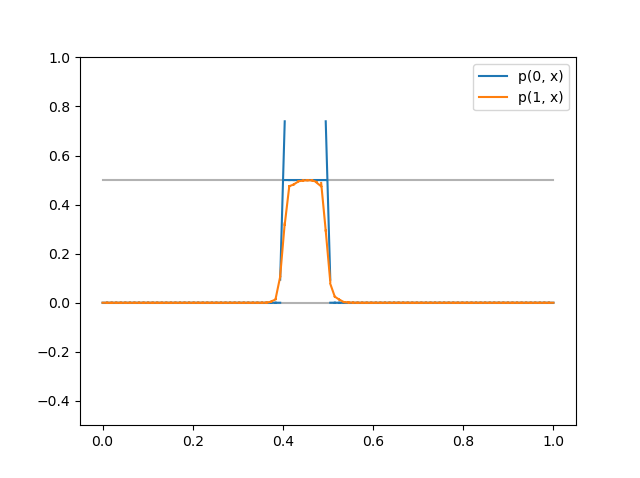
\includegraphics[width=\linewidth]{../figs/sols/adv1d_o2h100_limit}
		\caption{Limit: True}
	\end{subfigure}%
	\begin{subfigure}{.5\textwidth}
		\centering	
		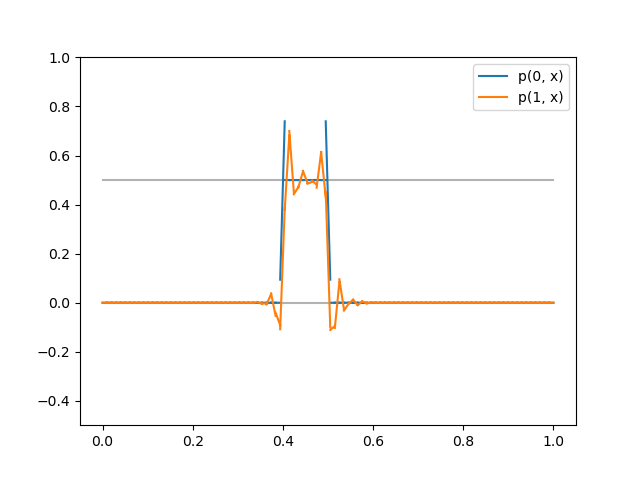
\includegraphics[width=\linewidth]{../figs/sols/adv1d_o2h100_nolimit}
		\caption{Limit: False}
	\end{subfigure}
	\caption{\Cref{ex:adv1D} Solution for $u_{step}$ for CFL coefficient $c=0.1$}
	\label{fig:sol_adv1D} 
\end{figure}

\begin{figure}[p!]
	\centering
	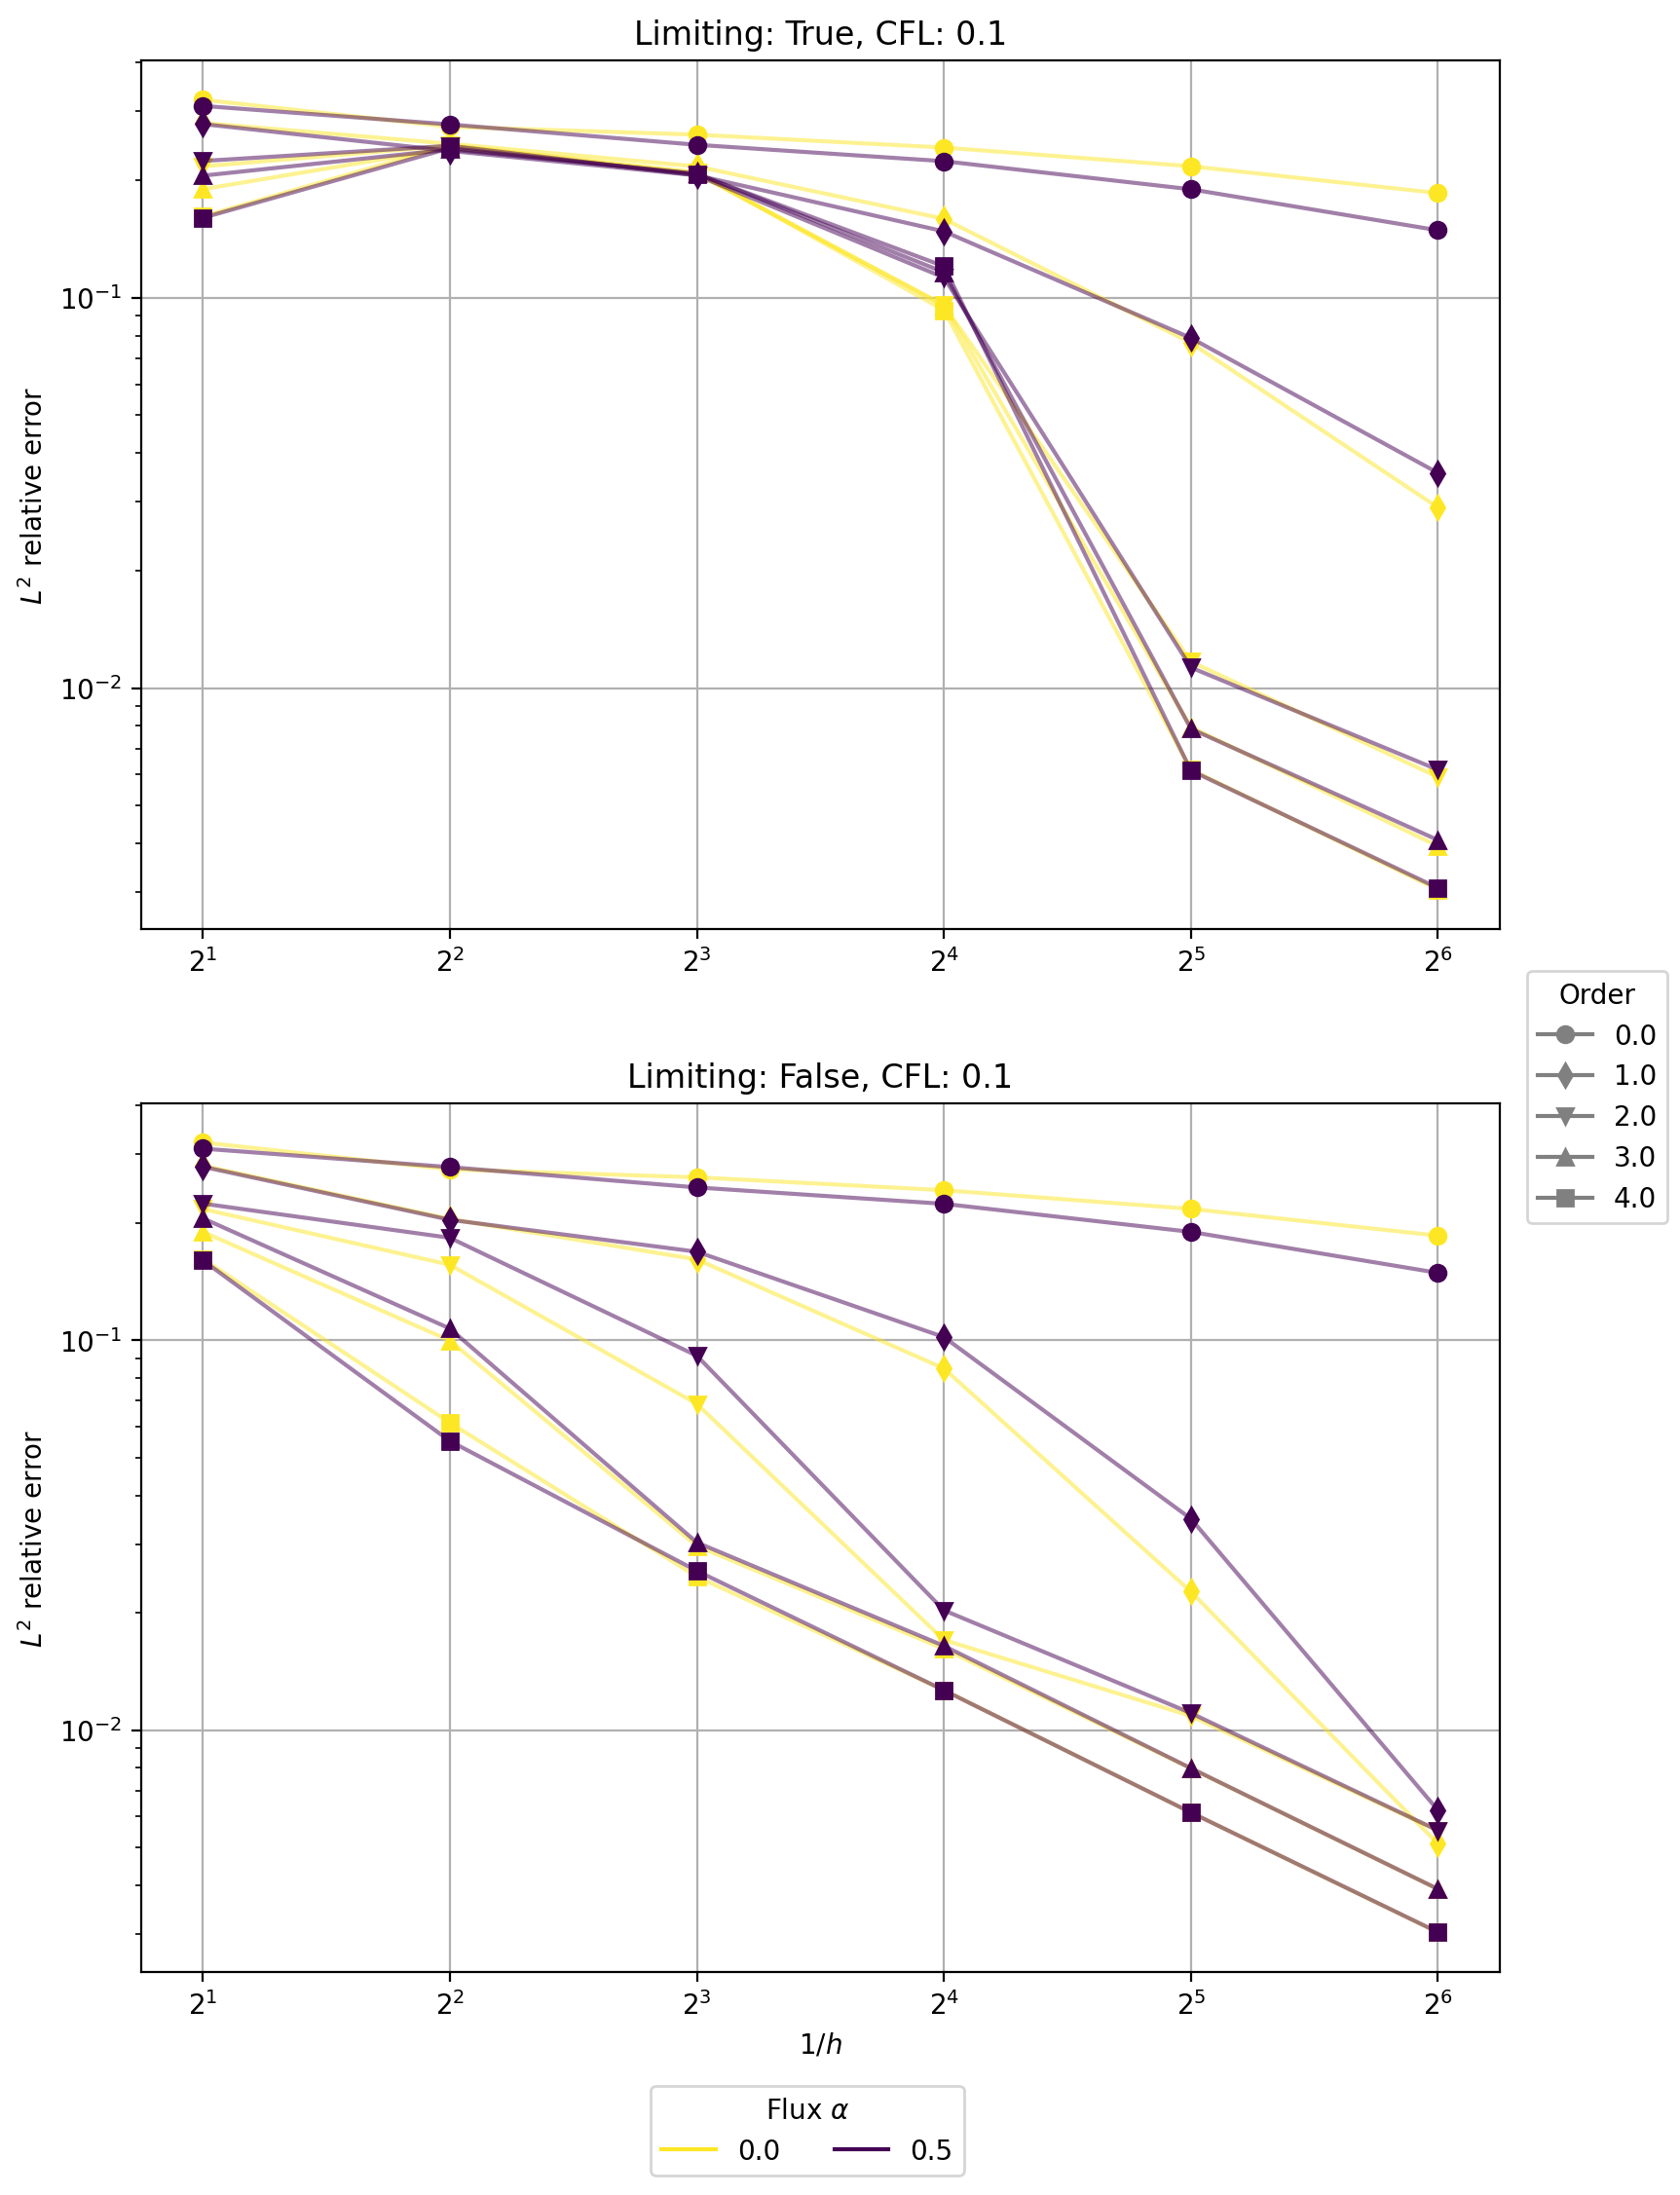
\includegraphics[width=1.1\textwidth]{../figs/parametric/advection_1D/advection_1D_smooth_reduced.png}
	\caption{\Cref{ex:adv1D} convergence plots for smooth initial condition 
		$u_{smooth}$}
	\label{fig:adv_conv_1D}
\end{figure}


\begin{figure}[p!]
	\centering
	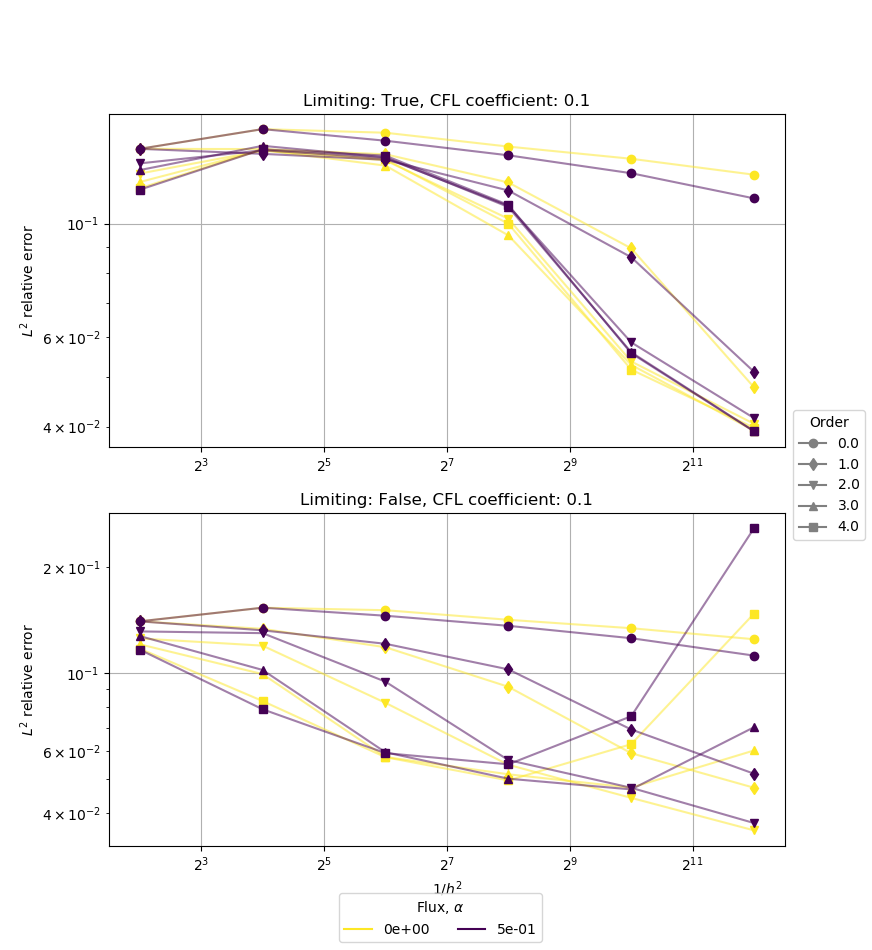
\includegraphics[width=1.1\textwidth]{../figs/parametric/advection_1D/advection_1D_step_reduced.png}
	\caption{\Cref{ex:adv1D} convergence plots for discontinuous initial 
	condition $u_{step}$}
	\label{fig:adv_conv_1D_step}
\end{figure}

\newpage
\begin{example}[Diffusion 2D]
\label{ex:laplace}
Inspired by \cite[cv. 8.4 (3), p. 150]{Holubova2011}, in $\Omega = \langle 0, 1 
\rangle^2$ 
we will solve Laplace equation \eqref{eq:ex_laplace}.
%\begin{equation}
%\pdiff{^2 u}{x^2} + \pdiff{^2 u}{y^2} = 0
%\end{equation}
%i.e
%\begin{equation}
%\Delta u = 0.
%\end{equation}
We setup boundary condition in such way that the exact solution 
$u_{exact}$ is polynomial
\begin{equation}
u_{exact} = \frac{1}{2}x^2 - \frac{1}{2}y^2 - ax + by + c.
\end{equation}
We set boundary conditions to match analytical solution as follows
\begin{equation}
	\begin{aligned}
		&u_x(0, y) = -a, & u_x(a, y) = 0\\
		&u_y(x, 0) = b, & u_y(x, b) = 0.
	\end{aligned}
\end{equation}
In our setting we chose $a=1$, $b=1$, $c=0$. Different values of 
coefficient $C_w$ in penalty term yield different convergence behavior as demonstrated in 
Figures \ref{fig:conv_laplace} and \ref{fig:orders_lapalce}.  \Cref{fig:orders_lapalce} 
may suggest that high order method do not meet expected convergence rate, they however 
still attain lowest error as illustrated in \Cref{fig:conv_laplace}. This is due to 
the polynomial solution which can be approximated very accurately even on coarse mesh and 
refining does not provide much benefit especially for high order approximations.
\end{example}

\begin{figure}[h!]
	\centering
	\begin{tabular}{p{0.5\textwidth} p{0.5\textwidth}}
		\vspace{0pt} 
        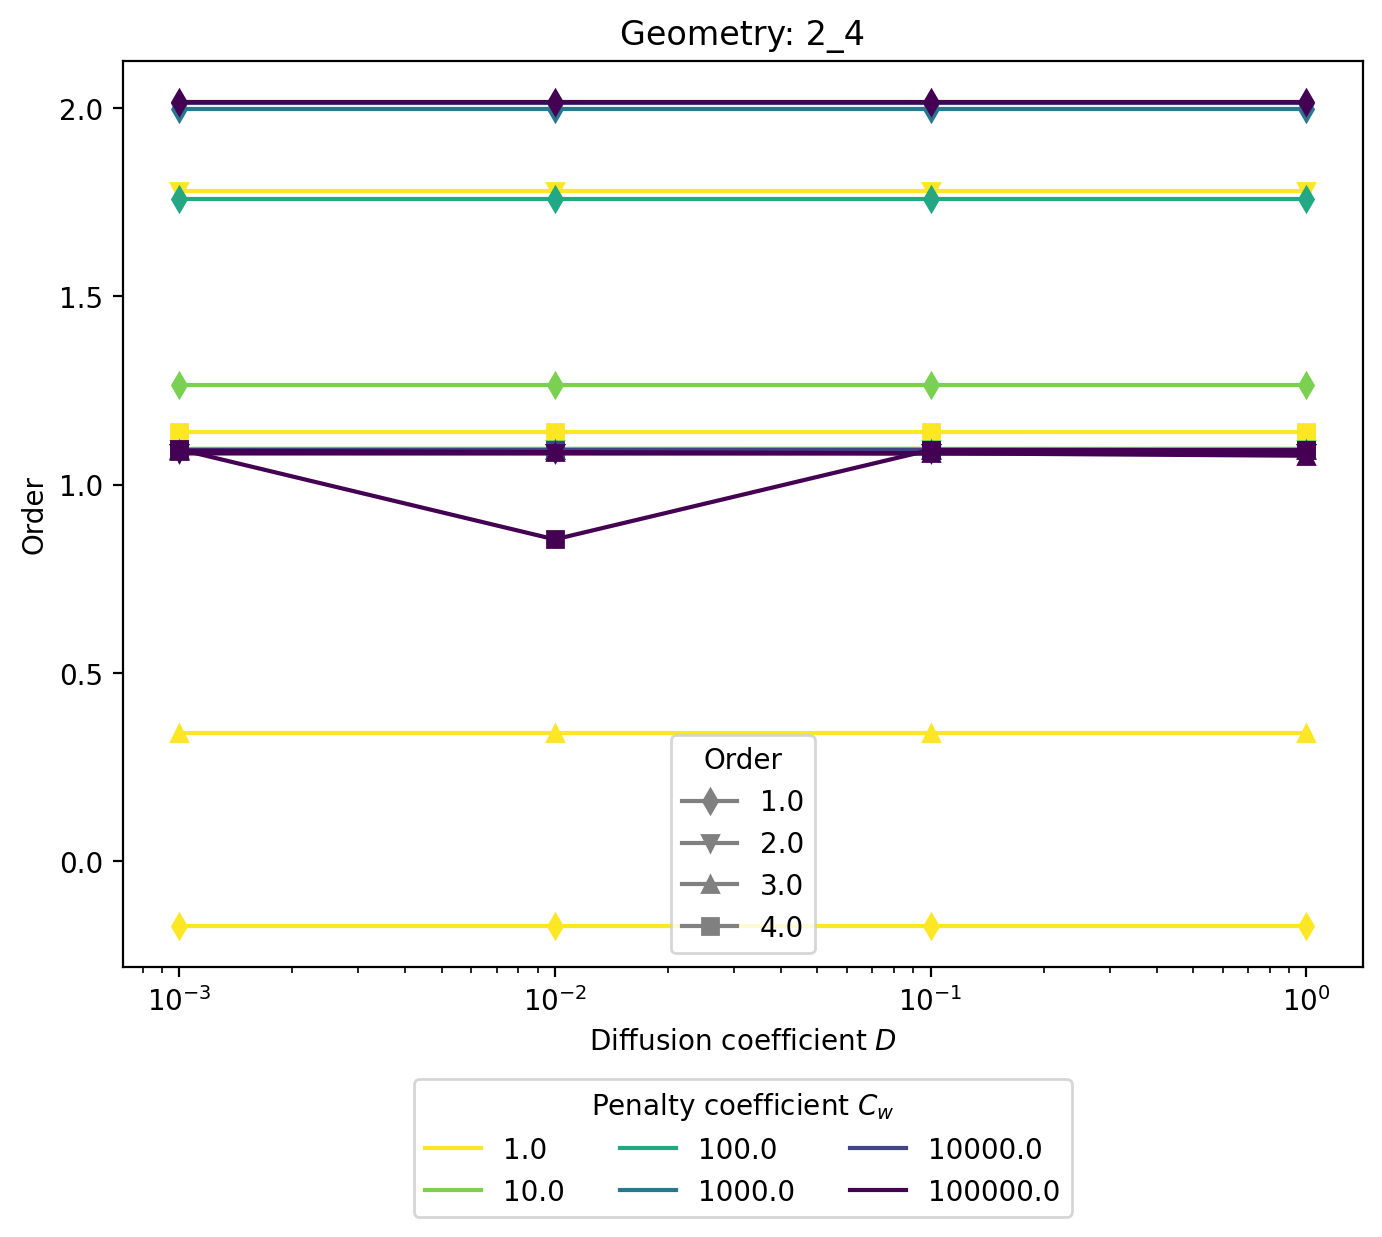
\includegraphics[width=0.49\textwidth]{../figs/parametric/diffusion_2D/ord_laplace_2_4}
		&
		\vspace{0pt} 
        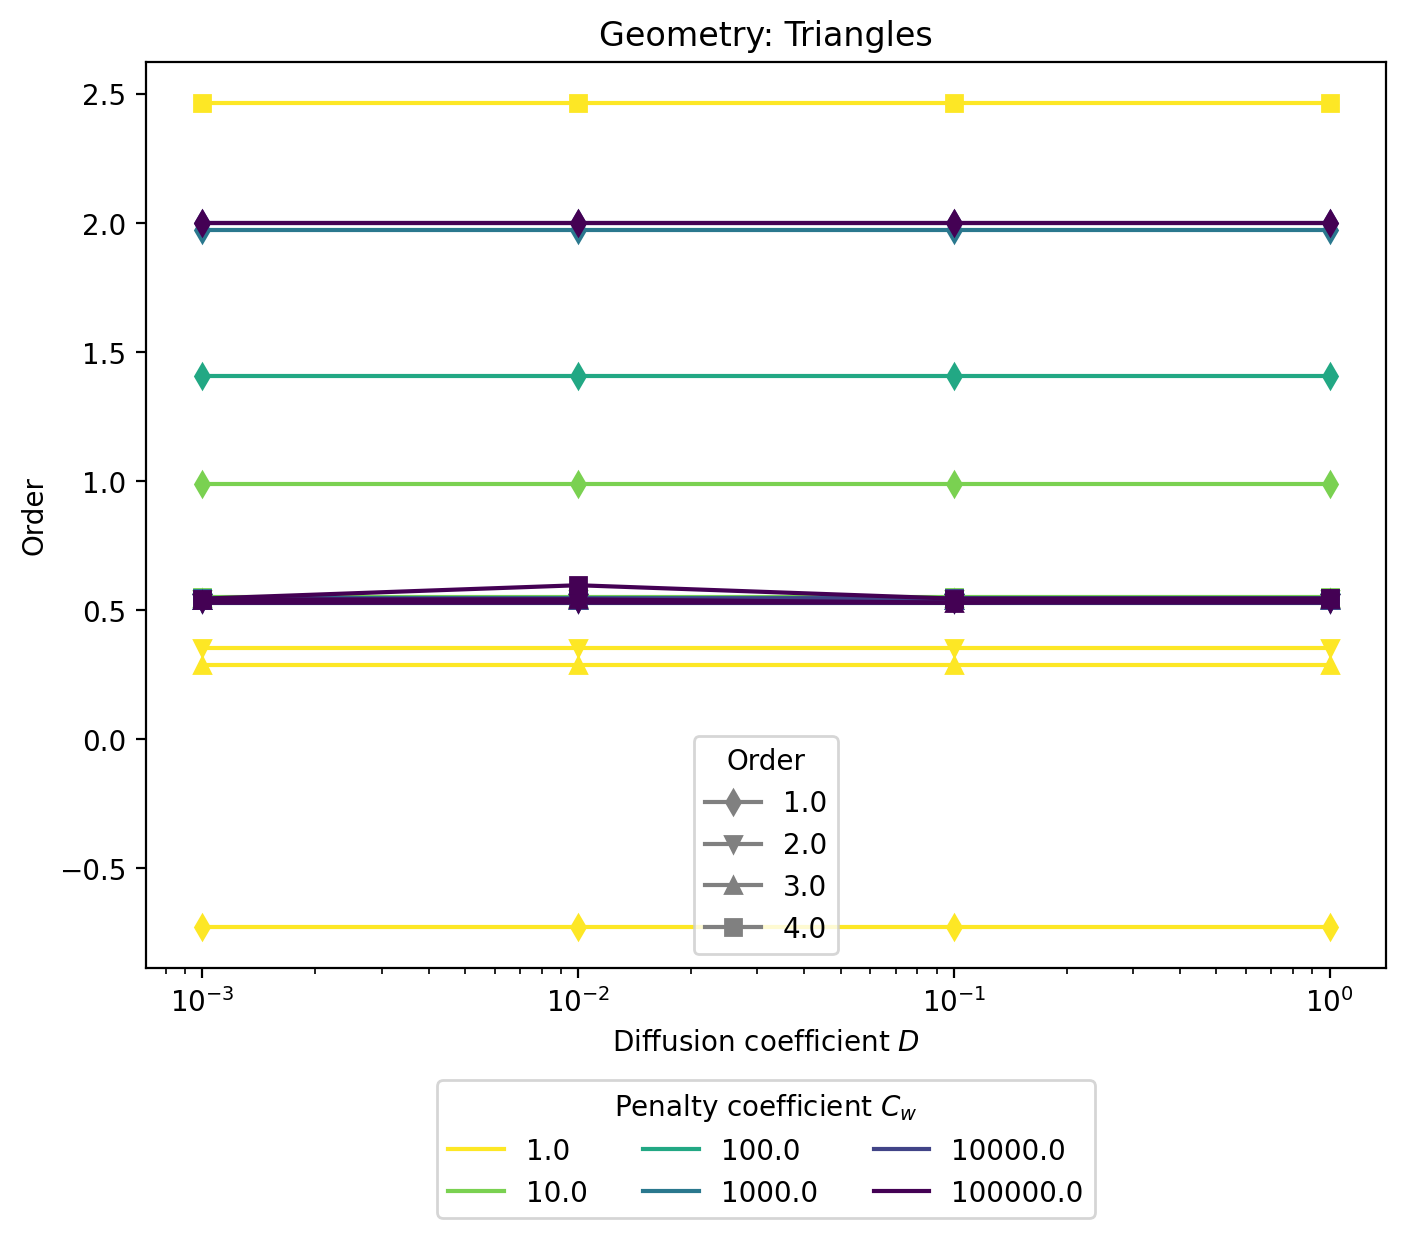
\includegraphics[width=0.49\textwidth]{../figs/parametric/diffusion_2D/ord_laplace_2_3}
	\end{tabular}
	\caption{\Cref{ex:laplace}. Average convergence rates for different choices of $C_w$ 
	for quadrilaterals (left) and triangles (right).}
	\label{fig:orders_lapalce}
\end{figure}

%\begin{figure}[h!]
%	\centering
%	\begin{subfigure}{.5\textwidth}	
%		\centering		
%        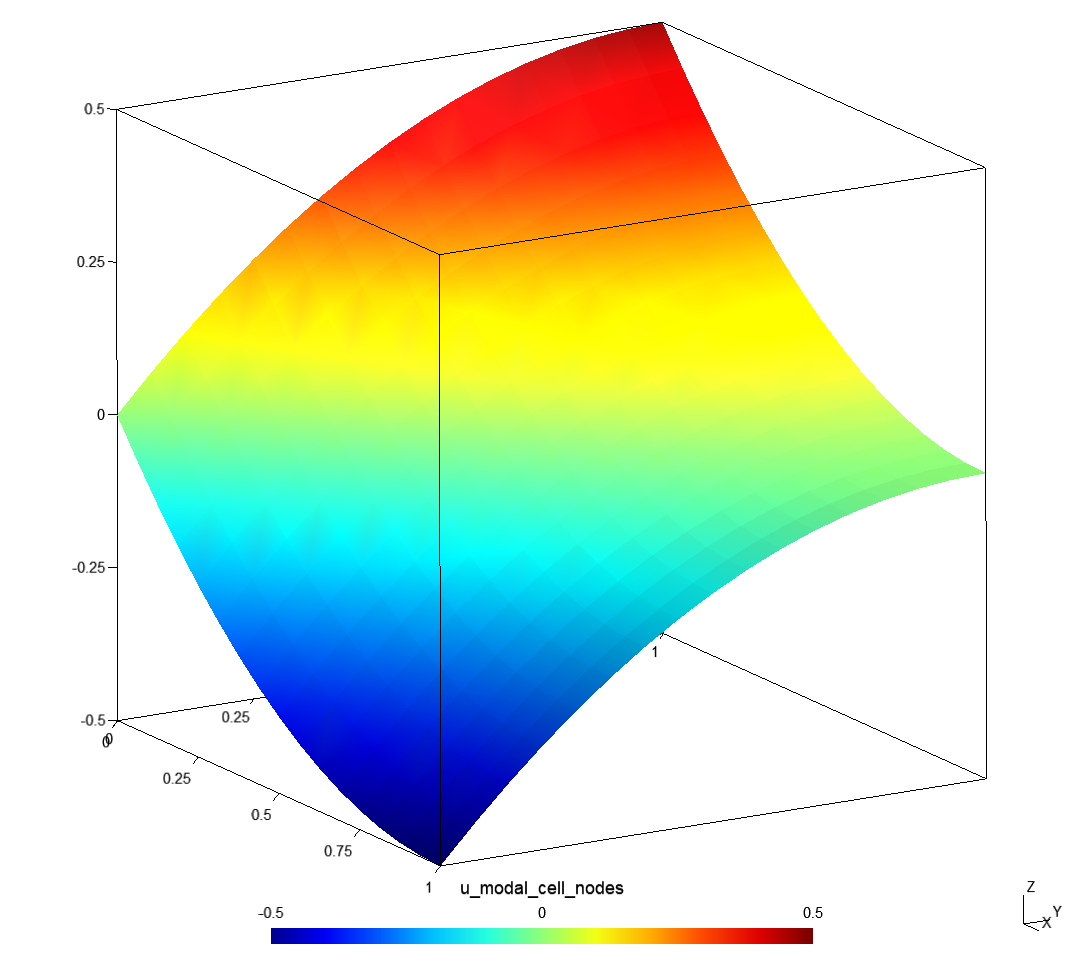
\includegraphics[width=\linewidth]{../figs/sols/laplace-52000-sol-h256o03.png}
%		\caption{??}
%	\end{subfigure}%
%%	\begin{subfigure}{.5\textwidth}
%%		\centering	
%%\includegraphics[width=\linewidth]{../figs/sols/}
%%		\caption{$C_w = 15$}
%%	\end{subfigure}
%	\caption{Solutions of \Cref{ex:laplace}  }
%\end{figure}

\begin{figure}[p!]
	\centering
	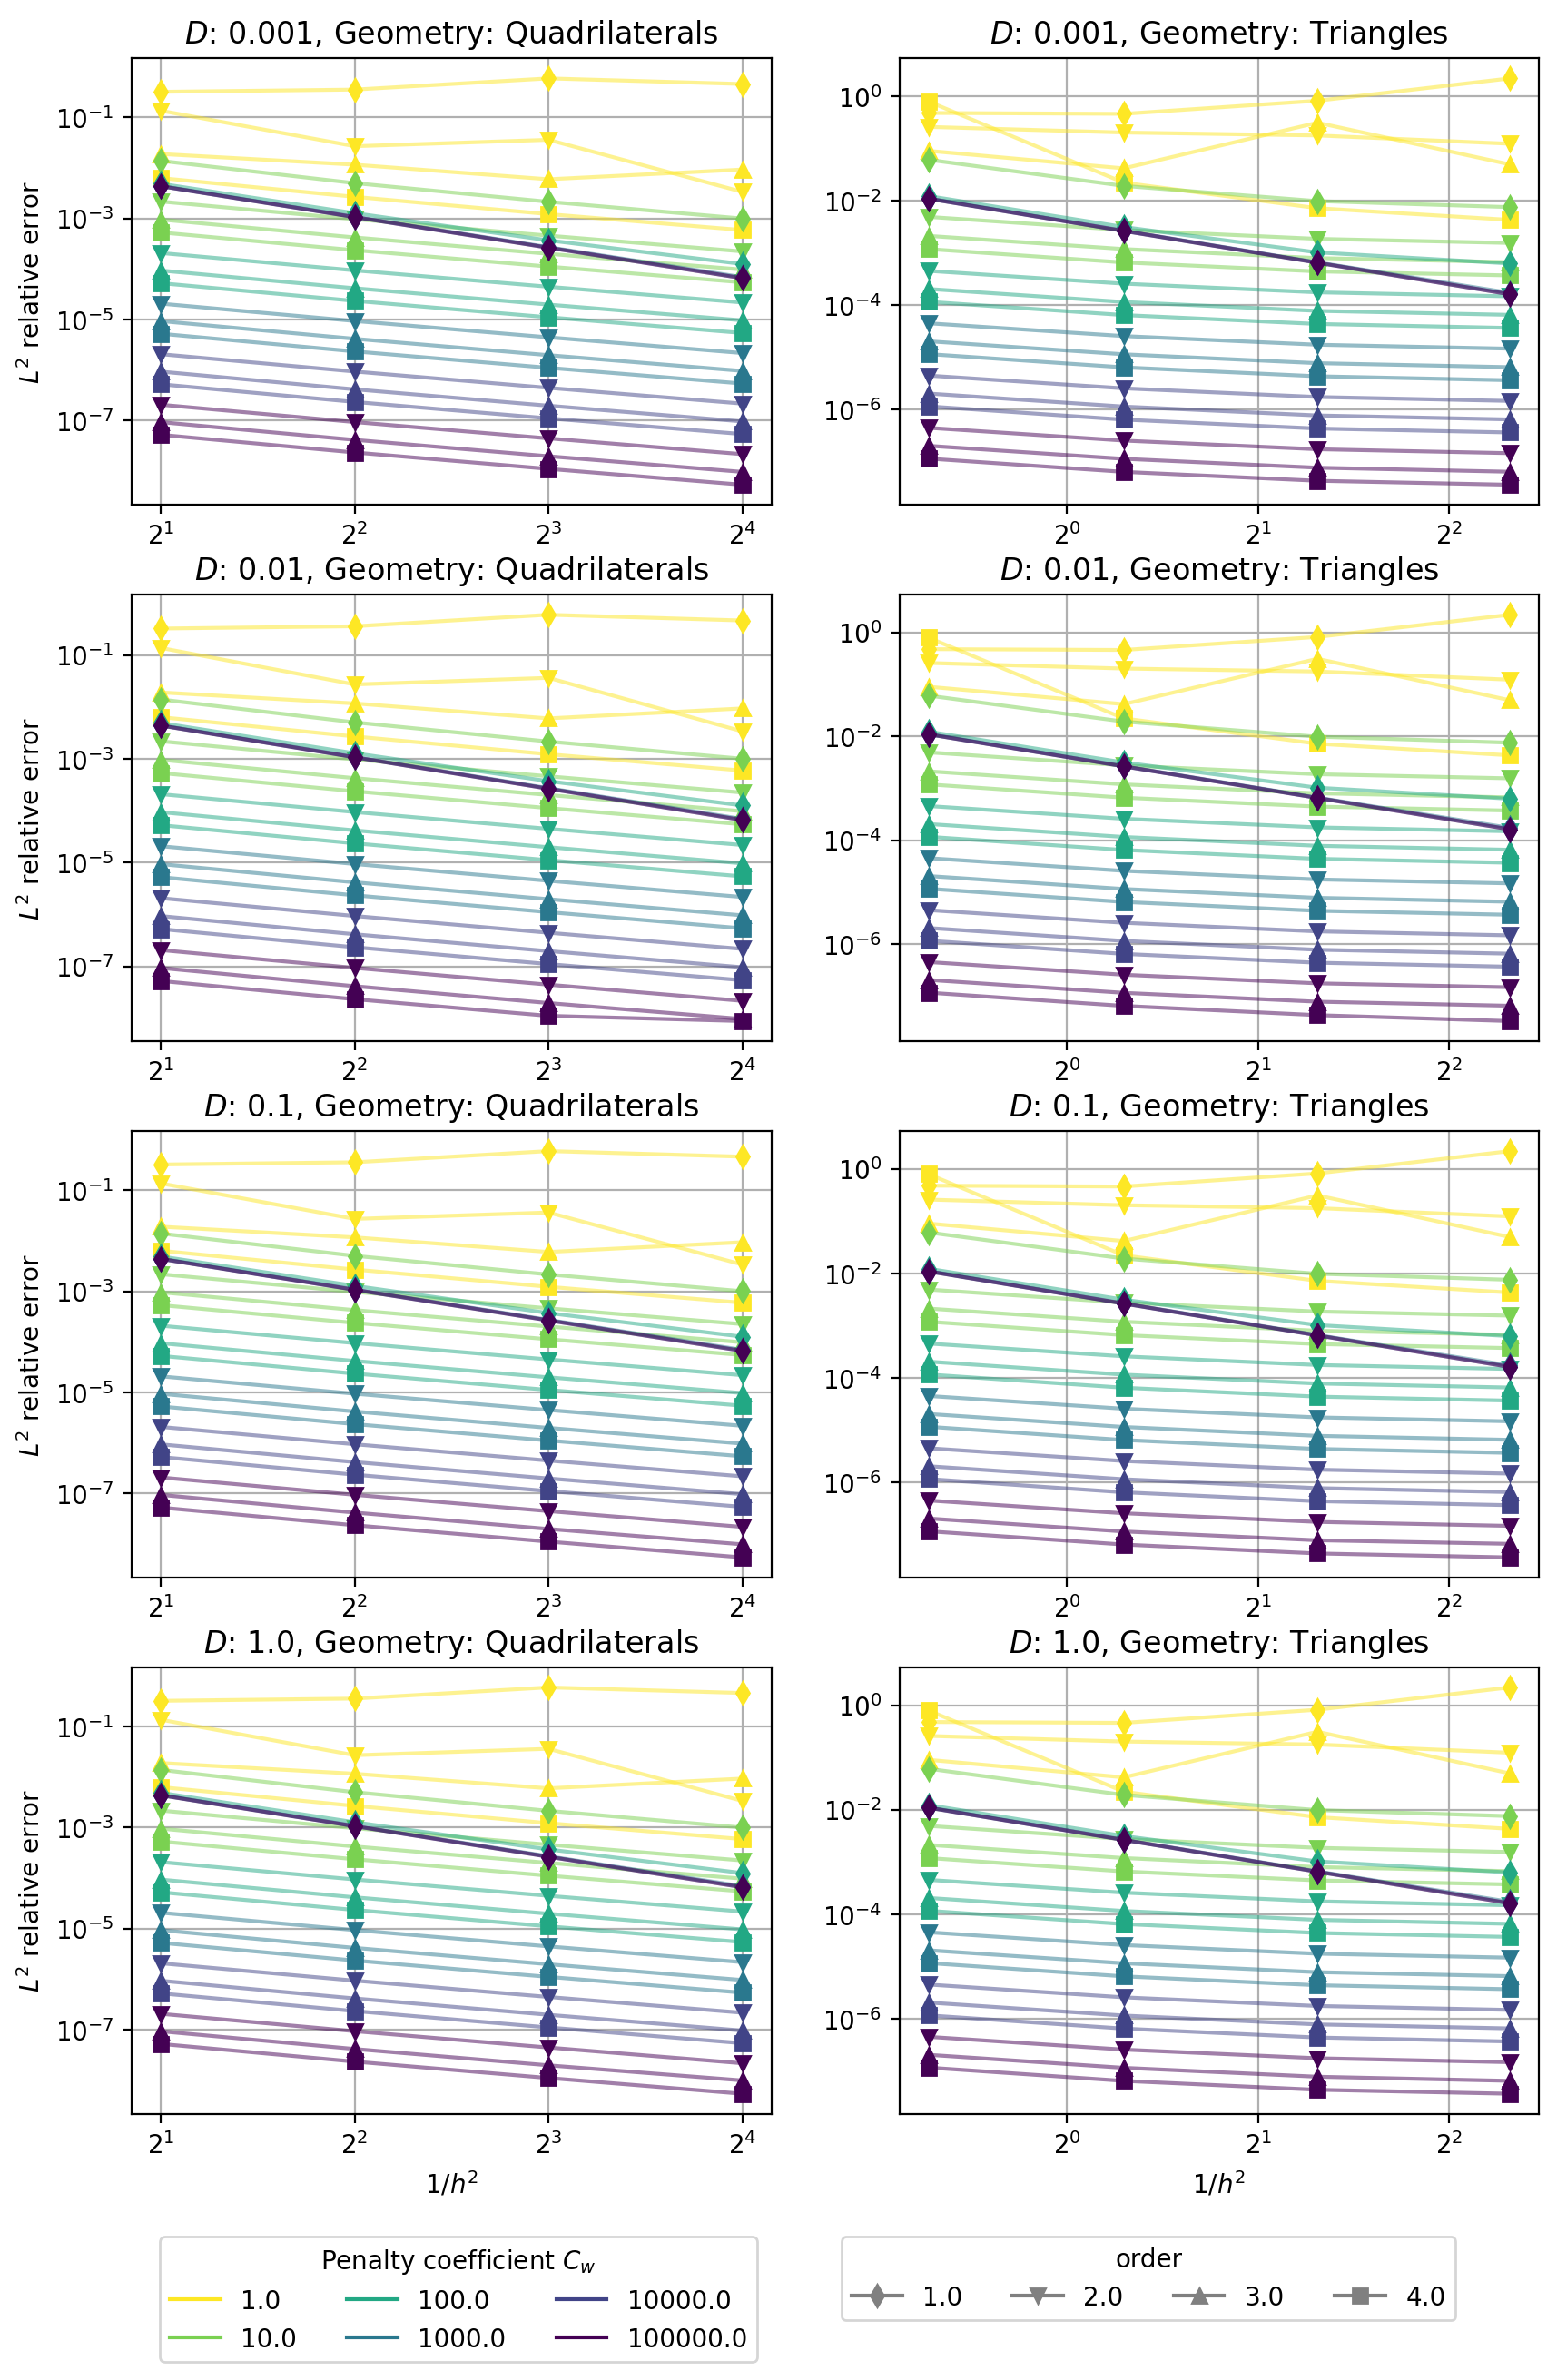
\includegraphics[height=\textheight]{../figs/parametric/diffusion_2D/laplace.png}
	\caption{\Cref{ex:laplace}. Relative errors for different choice of $C_w$  for 
		quadrilaterals (left) and triangles (right).}
	\label{fig:conv_laplace}
\end{figure}
\newpage
\begin{example}[Advection-diffusion 2D]
\label{ex:quart1}
Based on Example 1 from \cite{Antonietti2013},
we will solve equation \eqref{eq:ex_advdiff} in $\Omega = \langle 0, 1 \rangle^2$.
%\begin{equation}
%	\pdiff{u}{x} + \pdiff{u}{y} - D \cdot \left( \pdiff{^2 u}{x^2} + \pdiff{^2 
%u}{y^2} \right) = g
%\end{equation}
%i.e
%\begin{equation}
%	\vec{a} \cdot \nabla u - D \Delta u = g
%\end{equation}
%where $\vec{a} = [1, 1]^T$ is advection velocity, $D$ is diffusion coefficient 
%and $g$ is a source function.
We setup boundary conditions and source function $g$ in such way that 
the exact solution $u_{exact}$ is
\begin{equation}
	u_{exact}(x,y) =  -{\left(y^{2} - y\right)} \sin\left(2 \, \pi x\right).
\end{equation}
Solving for $g$ yields
\begin{equation}
	g = \\
	 -2 \, \pi {\left(y^{2} - y\right)} \cos\left(2 \, \pi x\right) - 2 \, {\left(2 \, 
	 \pi^{2} 
	{\left(y^{2} - y\right)} \sin\left(2 \, \pi x\right) - D\sin\left(2 \, \pi 
	x\right)\right)} 
	 - {\left(2 \, y - 1\right)} \sin\left(2 \, \pi x\right).
\end{equation}
matching  boundary conditions are
\begin{equation}
	\begin{aligned}
	&u(x) = 0, \quad x \in \partial\Omega\\
	&\nabla u(x) = [-2\pi(y^2 - y)\cos(2 \pi x), -(2 y - 1)\sin(2\pi  x)]^T, \quad x \in 
	\partial\Omega.
	\end{aligned}
\end{equation}
Different values of coefficient $C_w$ in penalty term then yield different 
convergence behavior as demonstrated in Figure \ref{fig:qconv1} and 
\Cref{fig:orders_quarteroni1}. Both figures illustrate "gluing" effect of penalty term 
which increases with $C_w$ coefficient and counteracts discontinuities between elements 
which are the main source of error in this example.

\begin{figure}[h!]
	\centering
	\begin{tabular}{p{0.5\textwidth} p{0.5\textwidth}}
		\vspace{0pt} 
		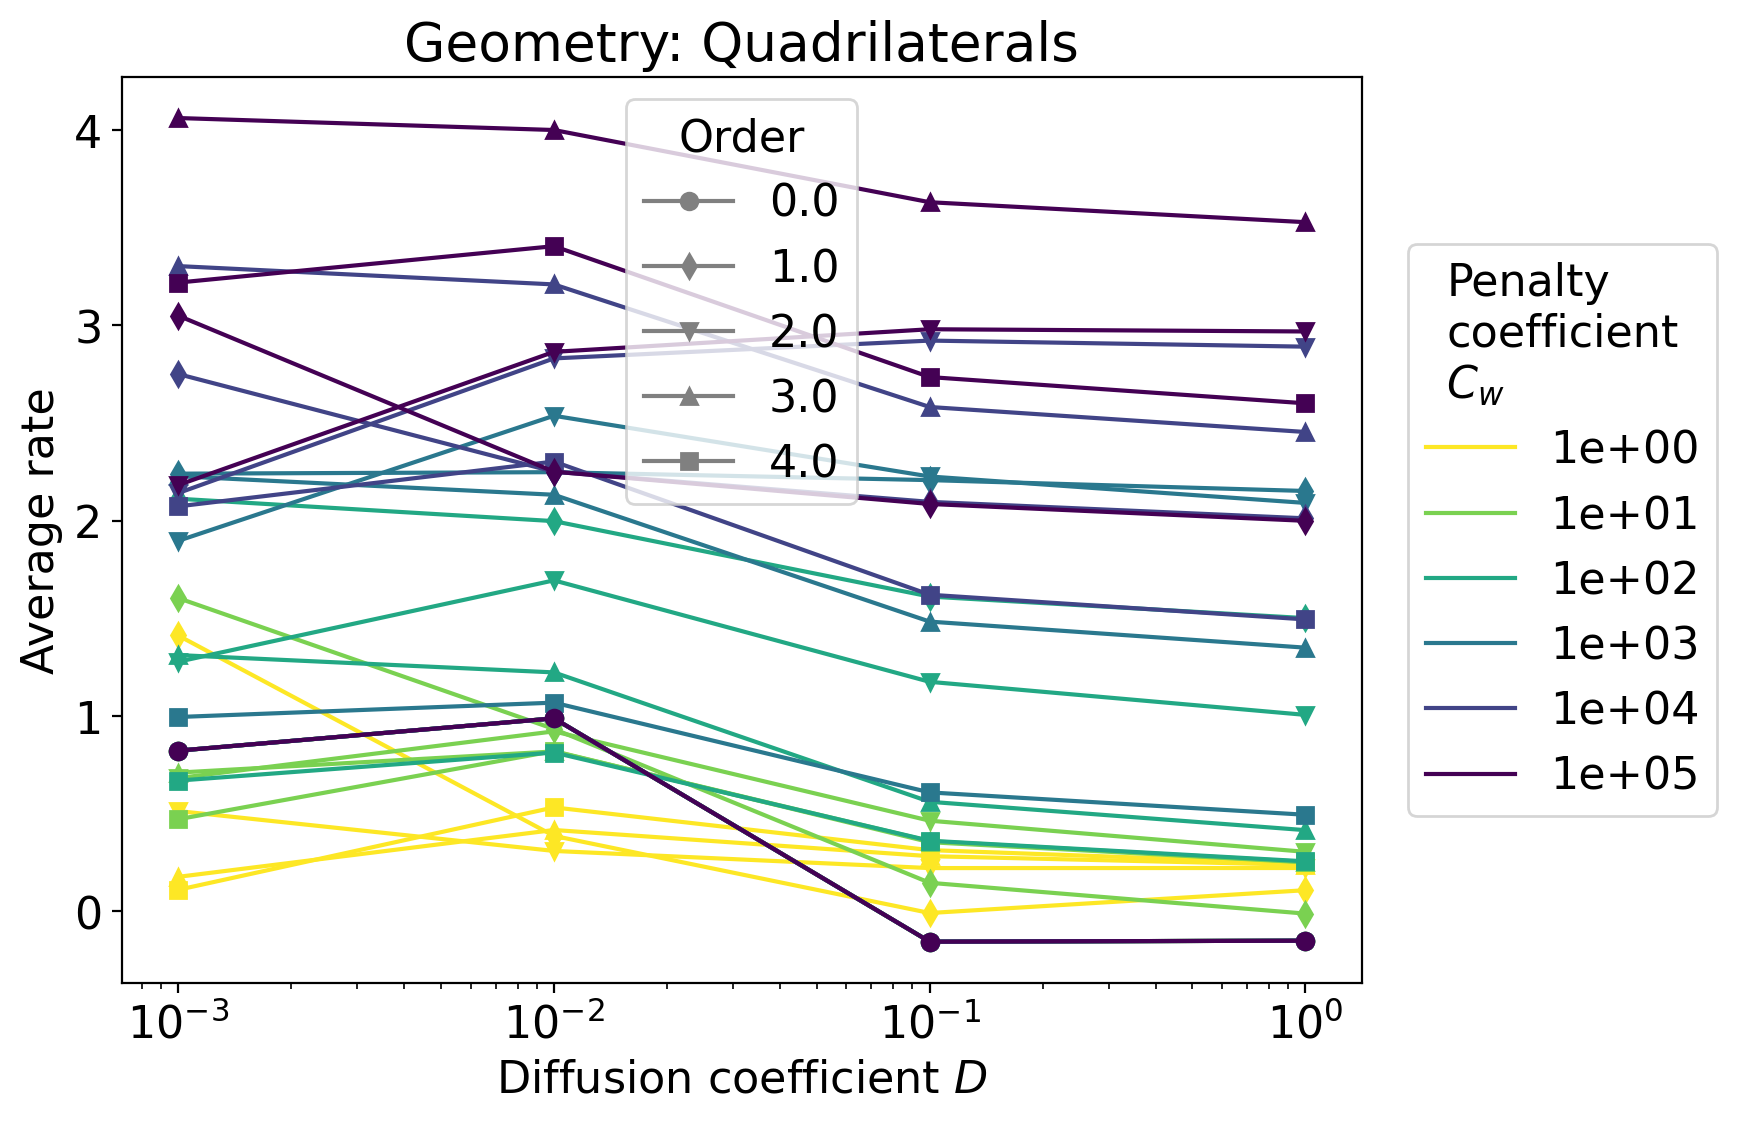
\includegraphics[width=0.49\textwidth]{../figs/parametric/advdiff_2D/ord_quarteroni1_2_4}
		&
		\vspace{0pt} 
		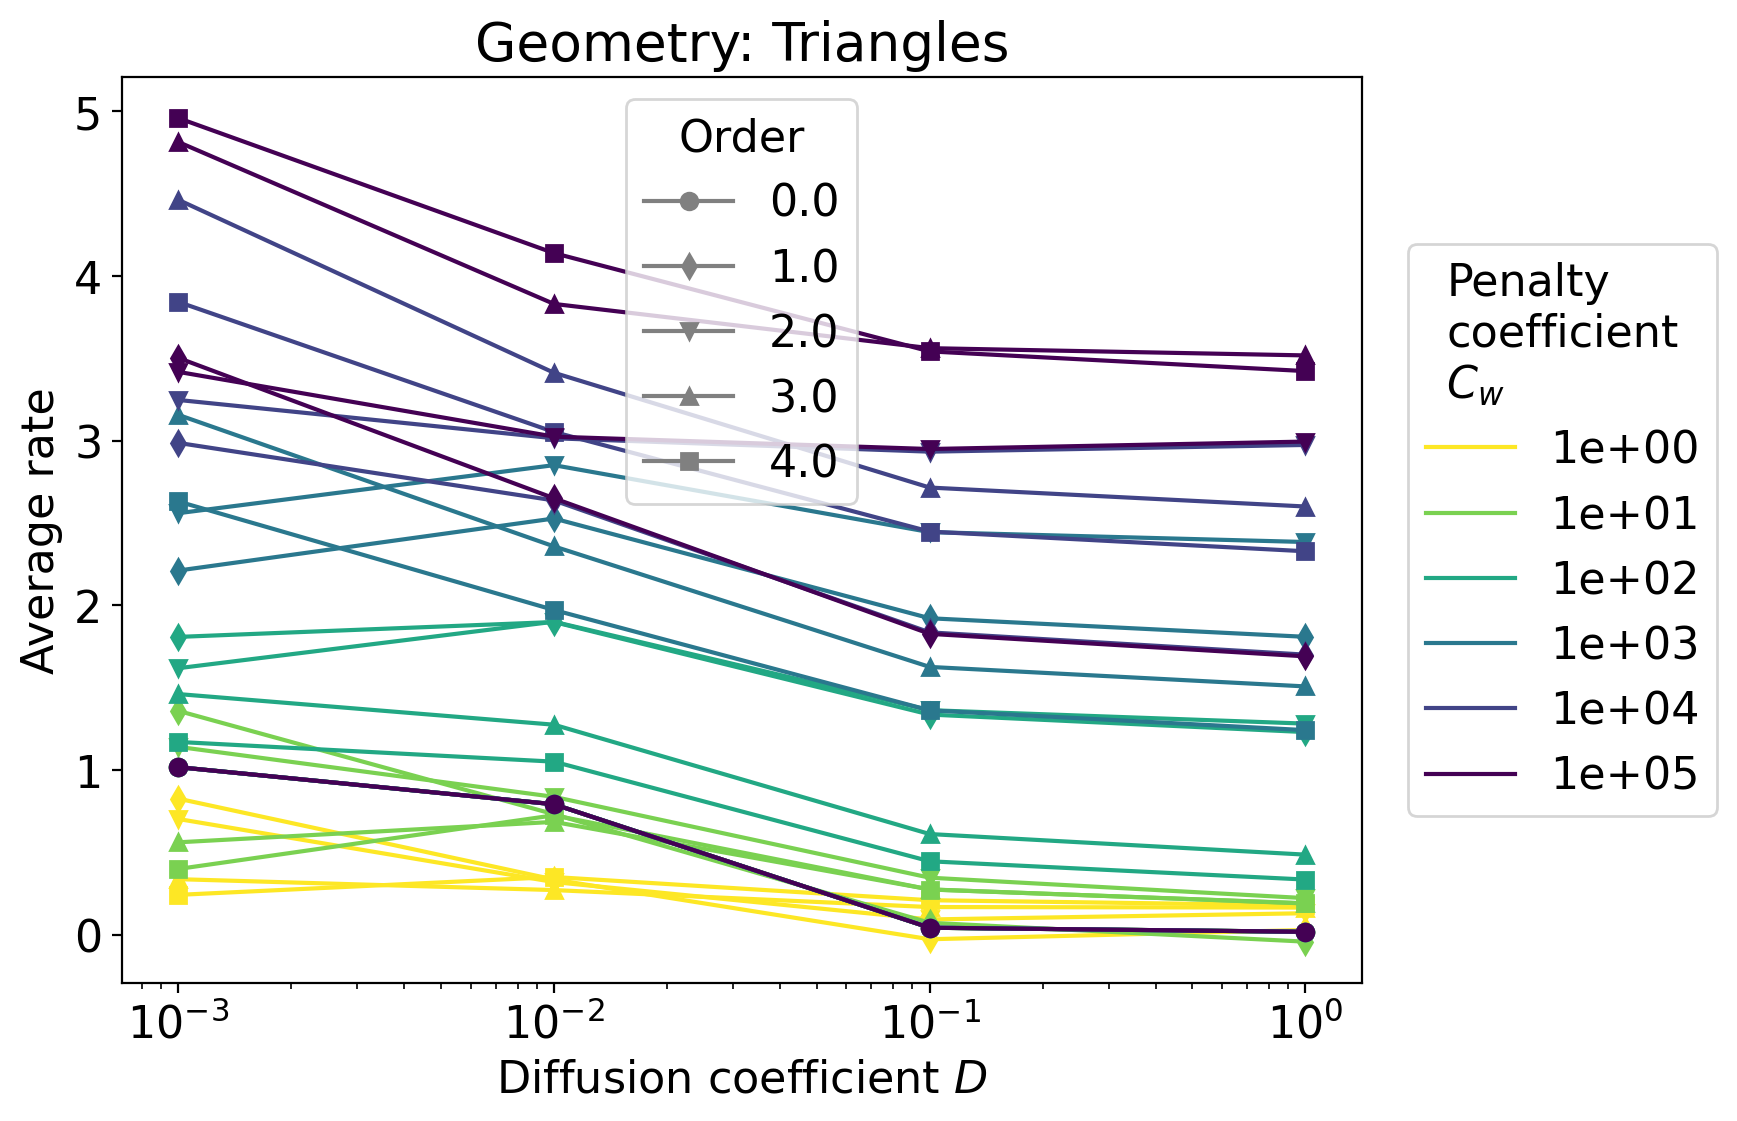
\includegraphics[width=0.49\textwidth]{../figs/parametric/advdiff_2D/ord_quarteroni1_2_3}
	\end{tabular}
	
%	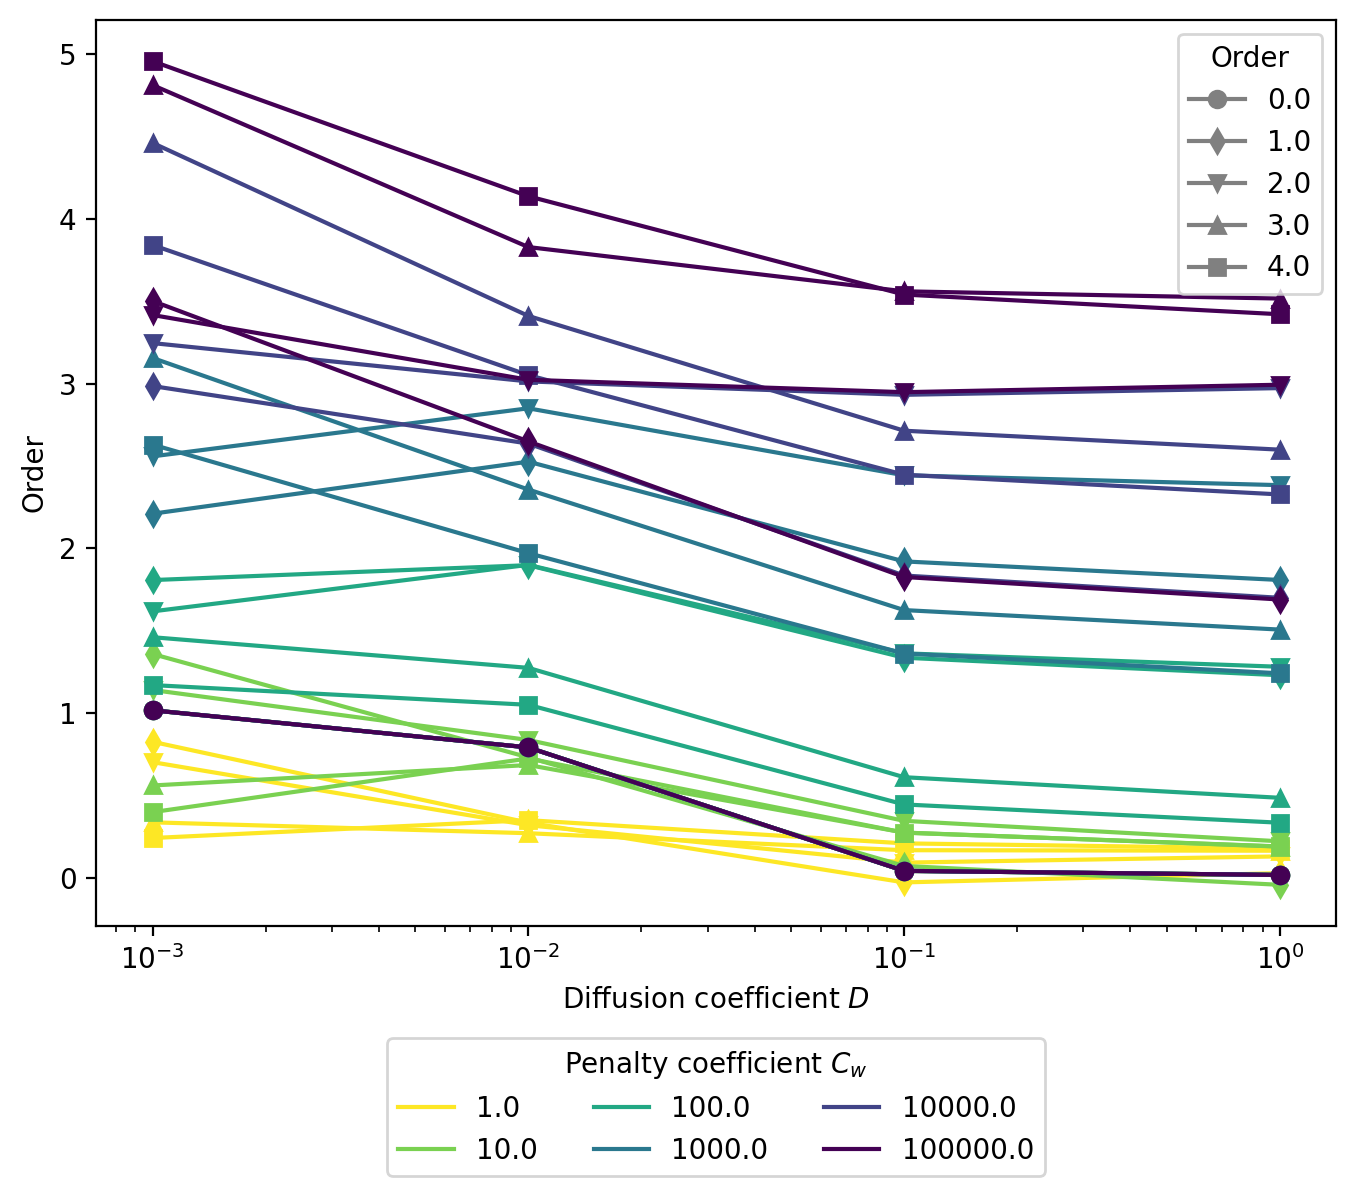
\includegraphics[scale=.5]{../figs/parametric/advdiff_2D/ord_quarteroni1}
	\caption{\Cref{ex:quart1} average order for different choice of $C_w$}
	\label{fig:orders_quarteroni1}
\end{figure}



\end{example}
\begin{figure}[p!]
	\centering
	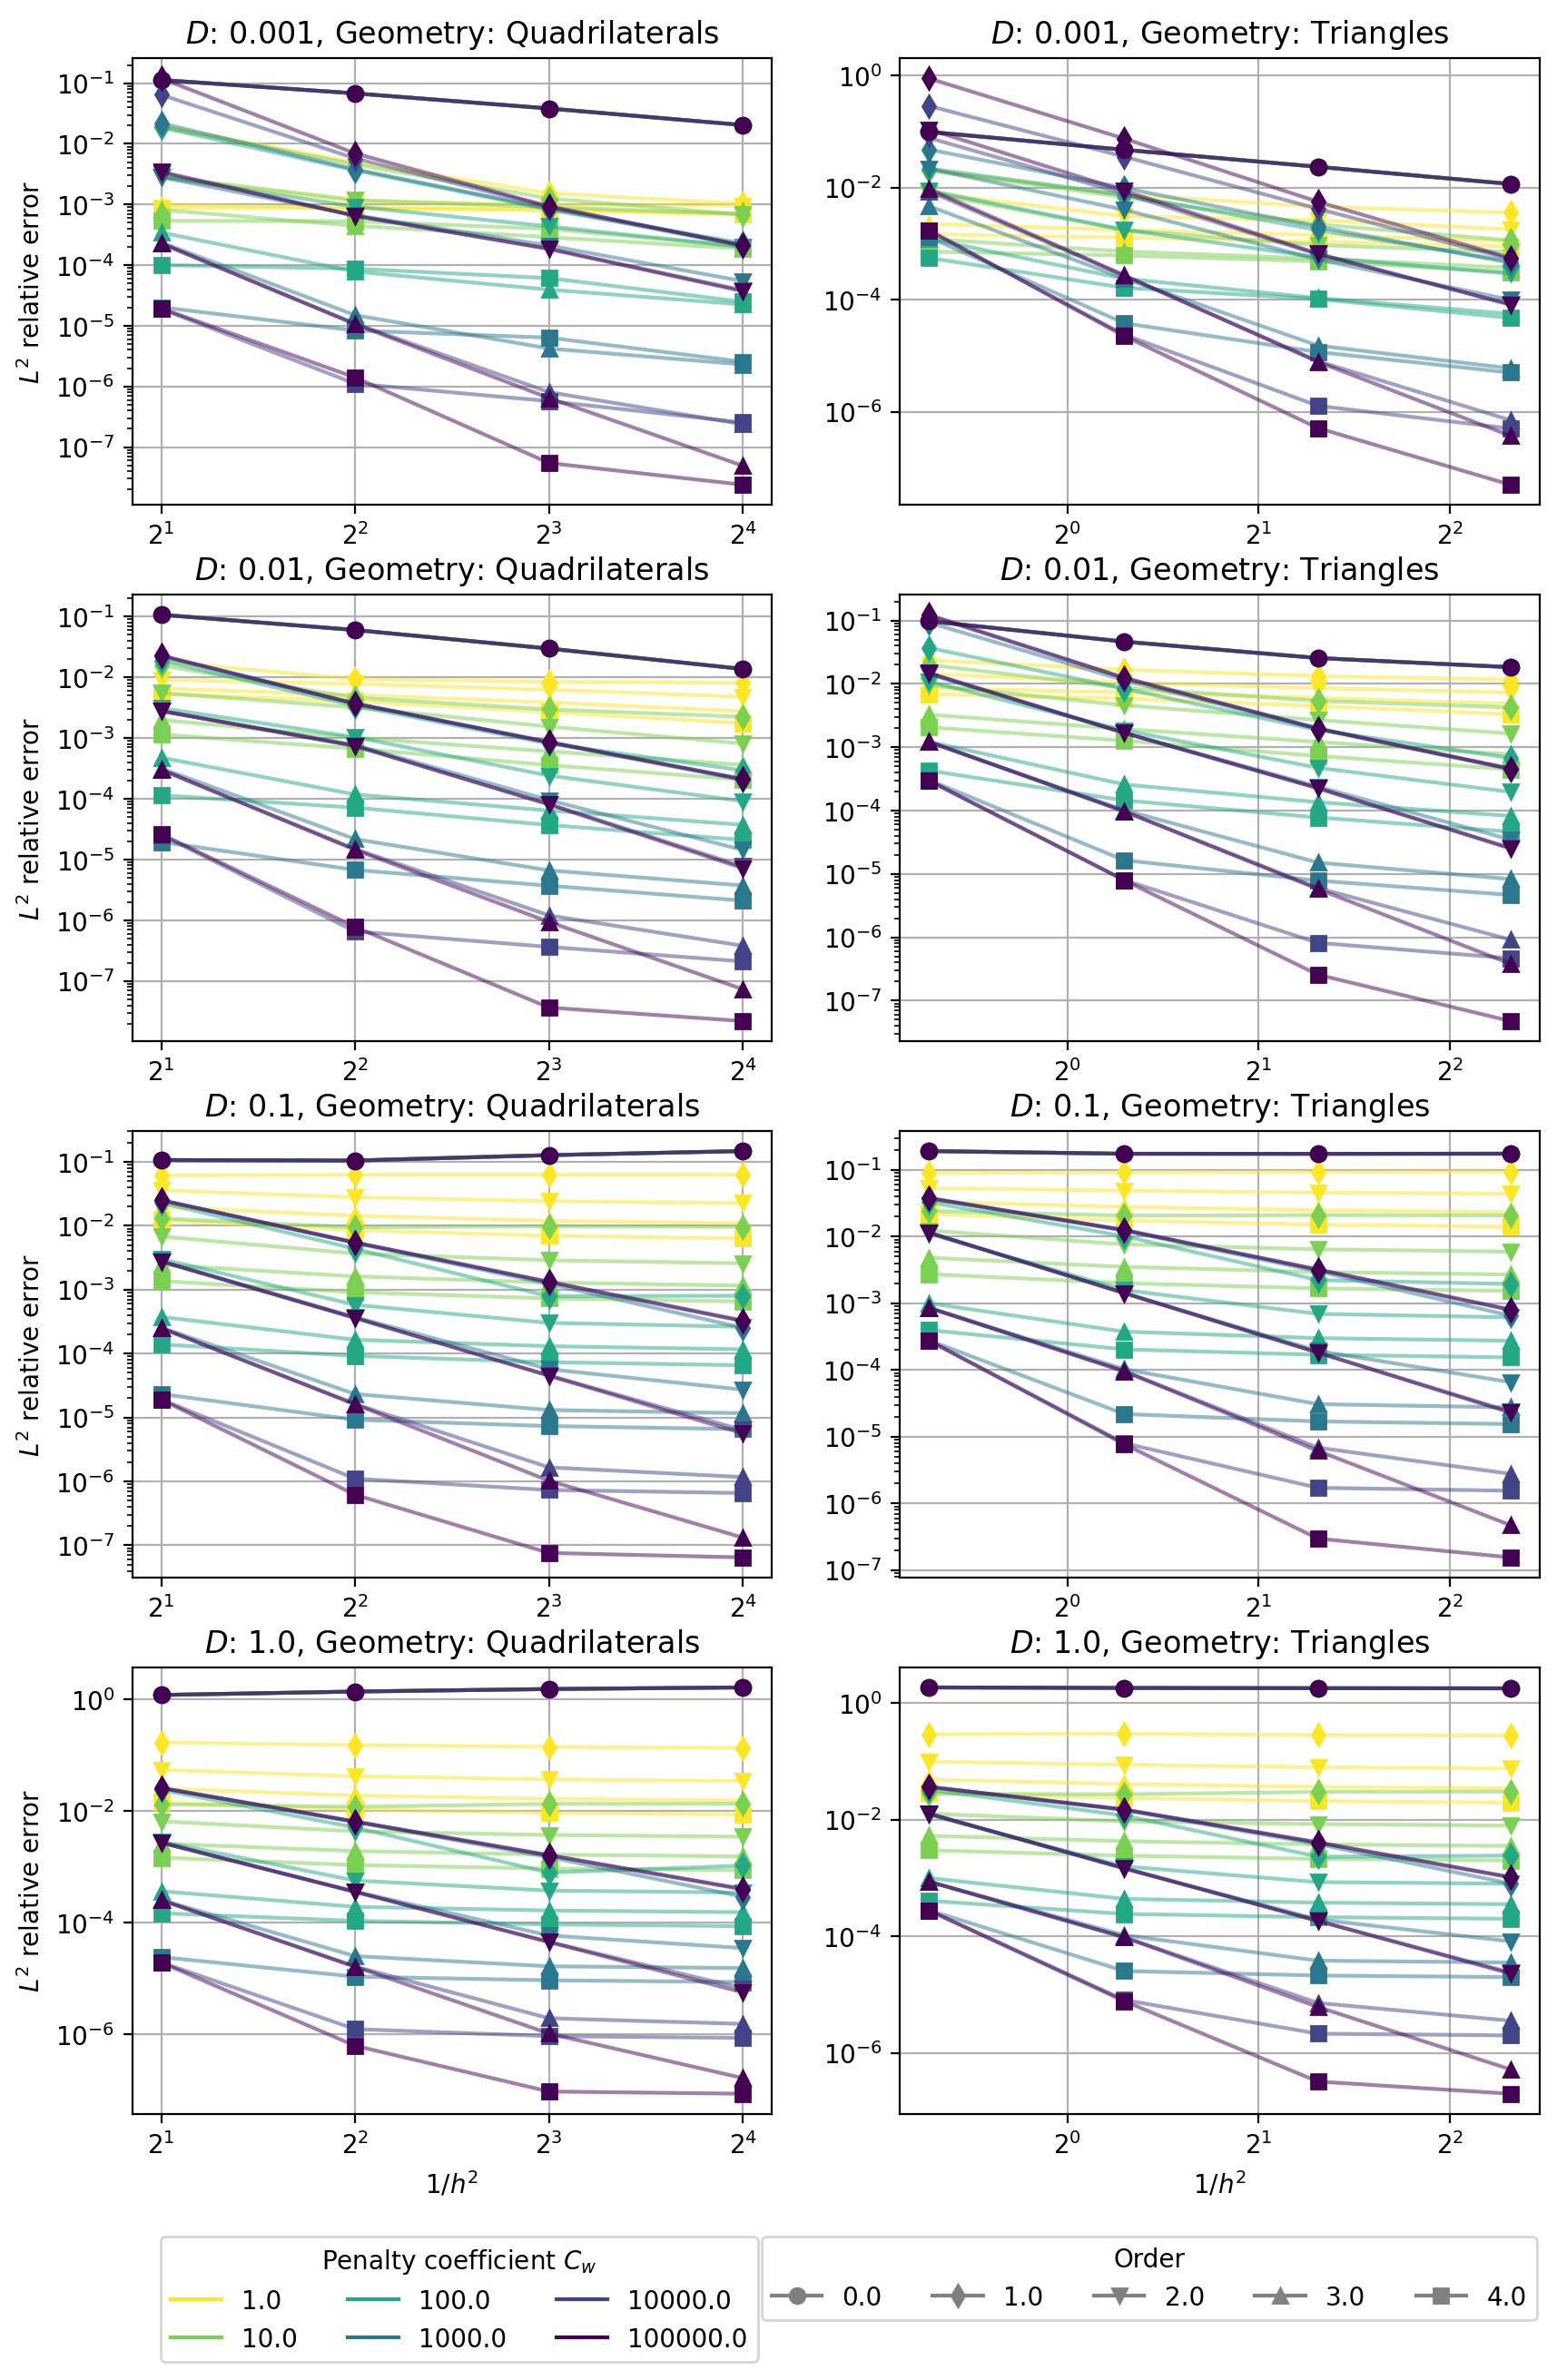
\includegraphics[height=\textheight]{../figs/parametric/advdiff_2D/quarteroni1}
	\caption{\Cref{ex:quart1} convergence graphs for different choice of $C_w$}
	\label{fig:qconv1}
\end{figure}

\newpage
\begin{example}[Advection-diffusion 2D]
\label{ex:quart2}
Based on Example 2 \cite{Antonietti2013},
in $\Omega = \langle 0, 1 \rangle^2$ we will again solve equation \eqref{eq:ex_advdiff}
%\begin{equation}
%	\pdiff{u}{x} + \pdiff{u}{y} - D \cdot \left( \pdiff{^2 u}{x^2} + \pdiff{^2 
%	u}{y^2} \right) = g
%\end{equation}
%i.e
%\begin{equation}
%	\vec{a} \cdot \nabla u - D \Delta u = g
%\end{equation}
%where $\vec{a} = [1, 1]^T$ is advection velocity and $D$ is diffusion 
%coefficient and $g$ is a source function. 
We setup boundary condition and source function in such way that the exact 
solution $u_{exact}$ is
\begin{equation}
	u_{exact} =  -\arctan\left(\frac{4 \, {\left(2 \, x - 1\right)}^{2} + 4 \, {\left(2 
	\, y - 1\right)}^{2} - 
	1}{16 \, \sqrt{\mathit{D}}}\right).
\end{equation}
We omit analytical forms of $g$ and boundary conditions for brevity, they can be found in 
the code.
Different values of coefficient $C_w$ in penalty term yield different 
convergence behavior as demonstrated in Figure \ref{fig:conv_qart2} and 
\Cref{fig:orders_quarteroni2}.
\end{example}

\begin{figure}[h!]
\centering
\begin{tabular}{p{0.5\textwidth} p{0.5\textwidth}}
	\vspace{0pt} 
	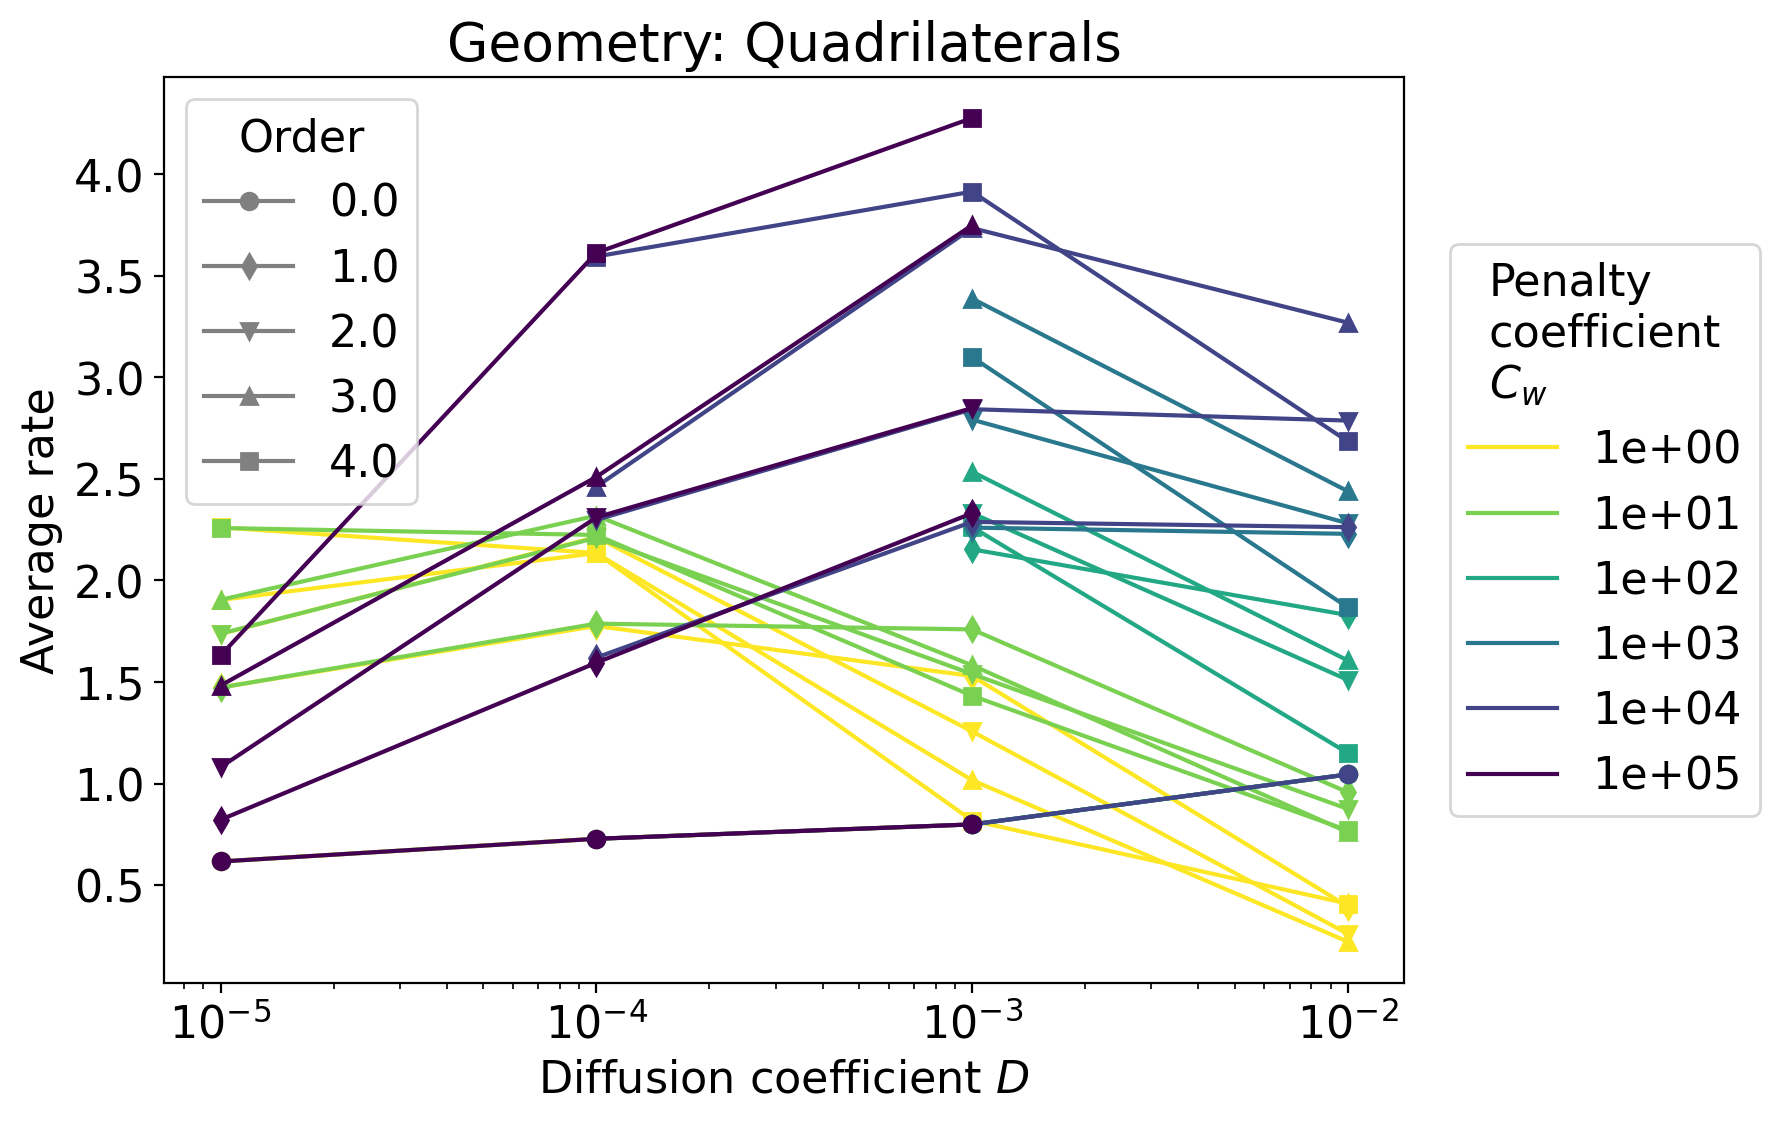
\includegraphics[width=0.49\textwidth]{../figs/parametric/advdiff_2D/ord_quarteroni2_2_4}
	&
	\vspace{0pt} 
	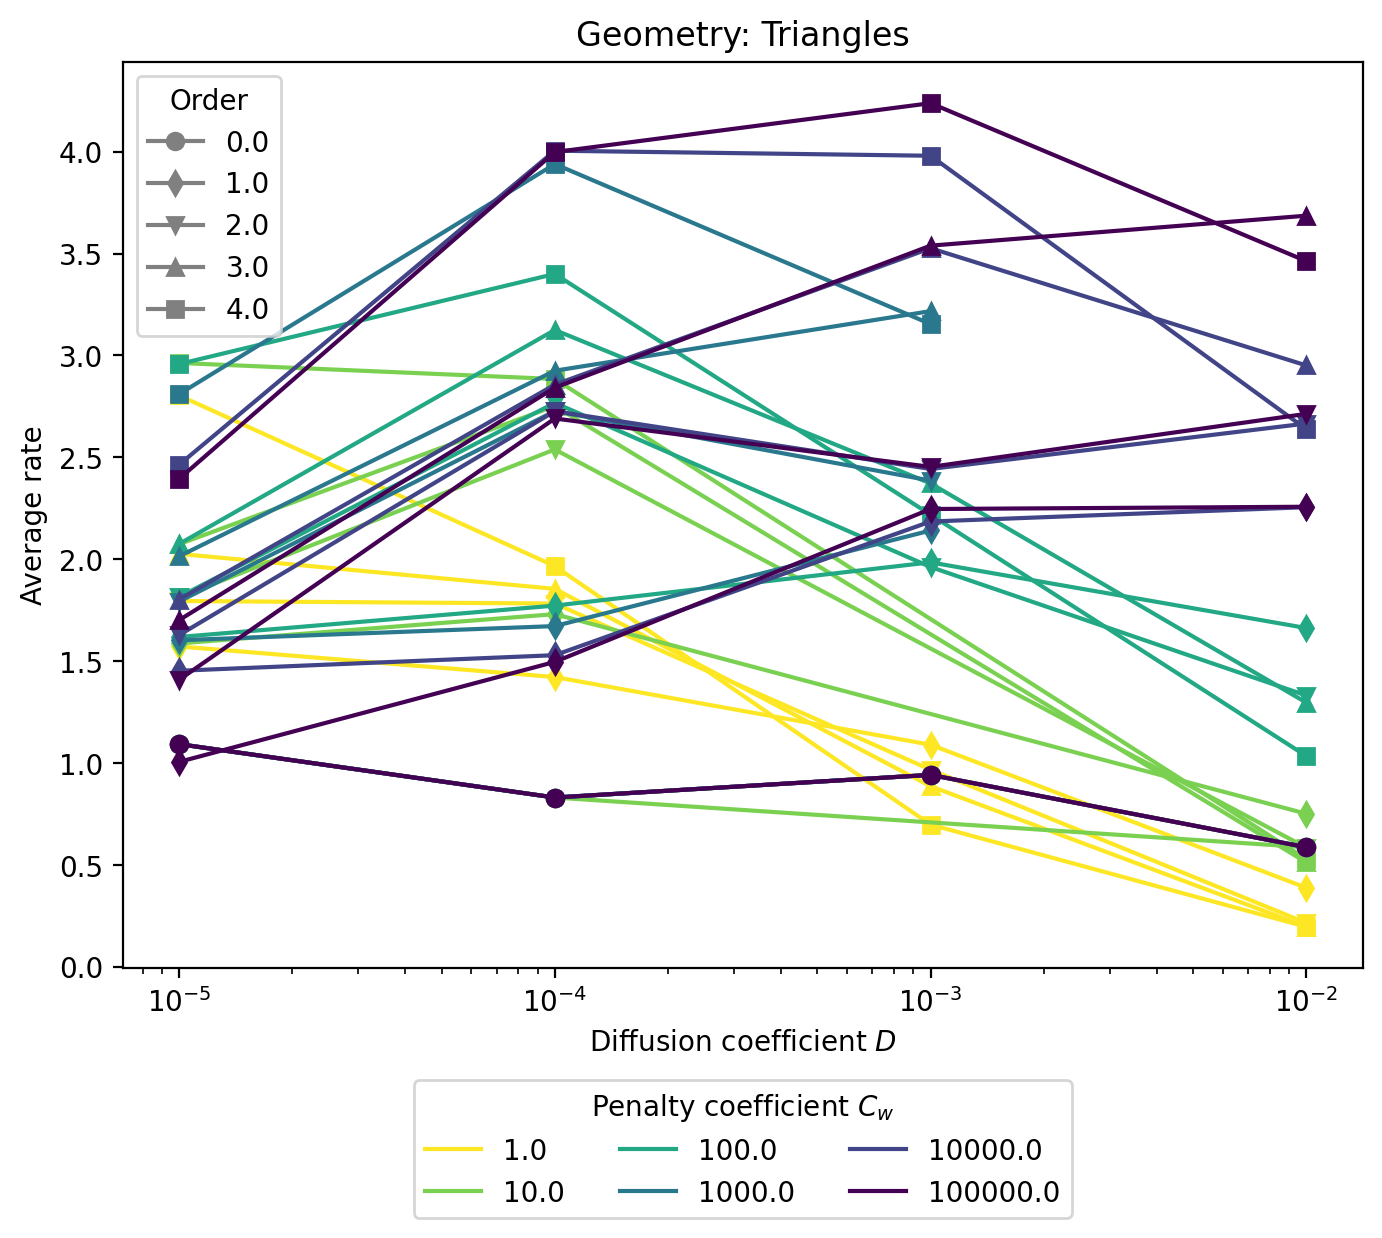
\includegraphics[width=0.49\textwidth]{../figs/parametric/advdiff_2D/ord_quarteroni2_2_3}
\end{tabular}
\caption{\Cref{ex:quart2} average order for different choice of $C_w$}
\label{fig:orders_quarteroni2}
\end{figure}


\begin{figure}[p!]
	\centering
	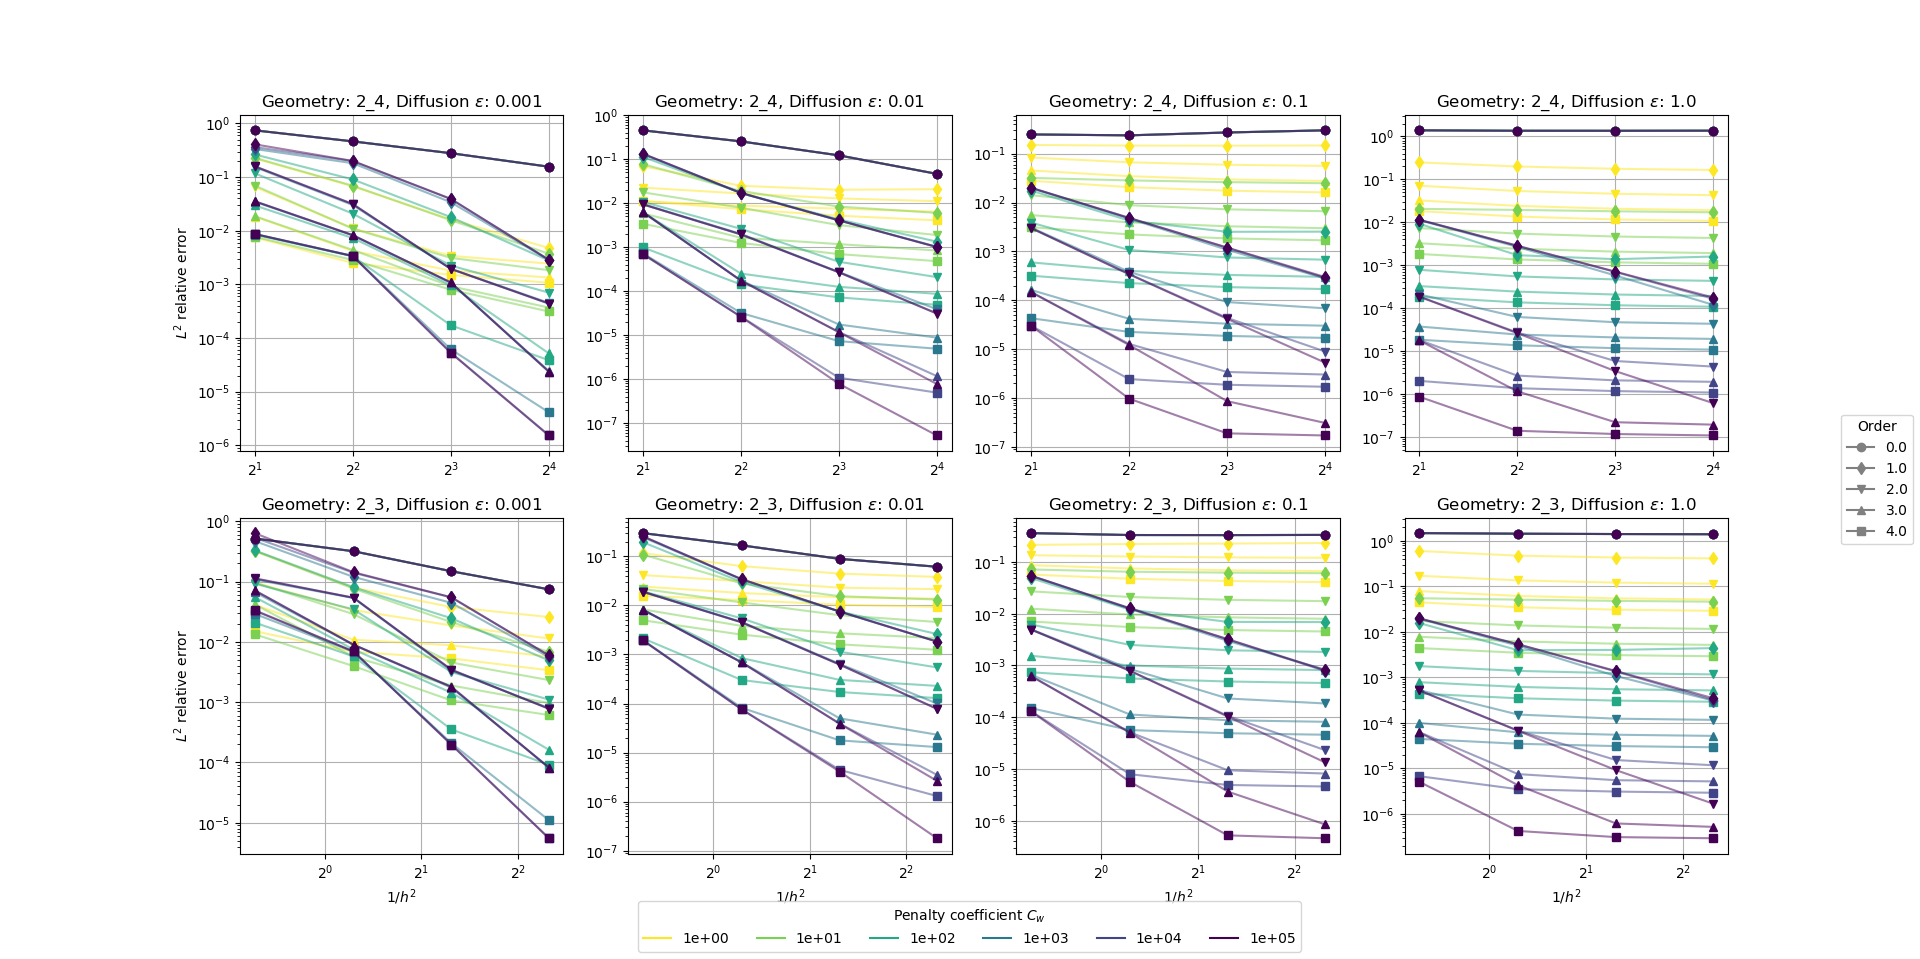
\includegraphics[height=\textheight]{../figs/parametric/advdiff_2D/quarteroni2.png}
	
	\caption{\Cref{ex:quart2} convergence graphs for different choice of $C_w$}
	\label{fig:conv_qart2}
\end{figure}

\newpage
\begin{example}[Advection-diffusion 2D]
\label{ex:quart3}
Based on Example 3 in \cite{Antonietti2013},
in $\Omega = \langle 0, 1 \rangle^2$ we will once again solve equation
%\begin{equation}
%	\pdiff{u}{x} + \pdiff{u}{y} - D \cdot \left( \pdiff{^2 u}{x^2} + \pdiff{^2 
%	u}{y^2} \right) = g
%\end{equation}
%i.e
%\begin{equation}
%	\vec{a} \cdot \nabla u - D \Delta u = g
%\end{equation}
%where $\vec{a} = [1, 1]^T$ is advection velocity and $D$ is diffusion 
%coefficient and $g$ is a source function.
We set up boundary condition and source function in such a way that the exact 
solution $u_{exact}$ is
\begin{equation}
	u_{exact} = -xy + x +y + \frac{\exp{\left(-\frac{{\left(x - 1\right)} {\left(y - 
	1\right)}}{D}\right)} - 
	\exp{\left(-\frac{1}{D}\right)}}{\exp{\left(-\frac{1}{D}\right)} 
	- 1}.
\end{equation}
We omit analytical forms of $g$ and boundary conditions for brevity, they can found in 
the code. Different values of 
coefficient $C_w$ in penalty term yield different convergence behavior as 
demonstrated in Figure 
\ref{fig:conv_qart3} and \Cref{fig:orders_quarteroni3}
\end{example}

\begin{figure}[h!]
	\centering
	\begin{tabular}{p{0.5\textwidth} p{0.5\textwidth}}
	\vspace{0pt} 
	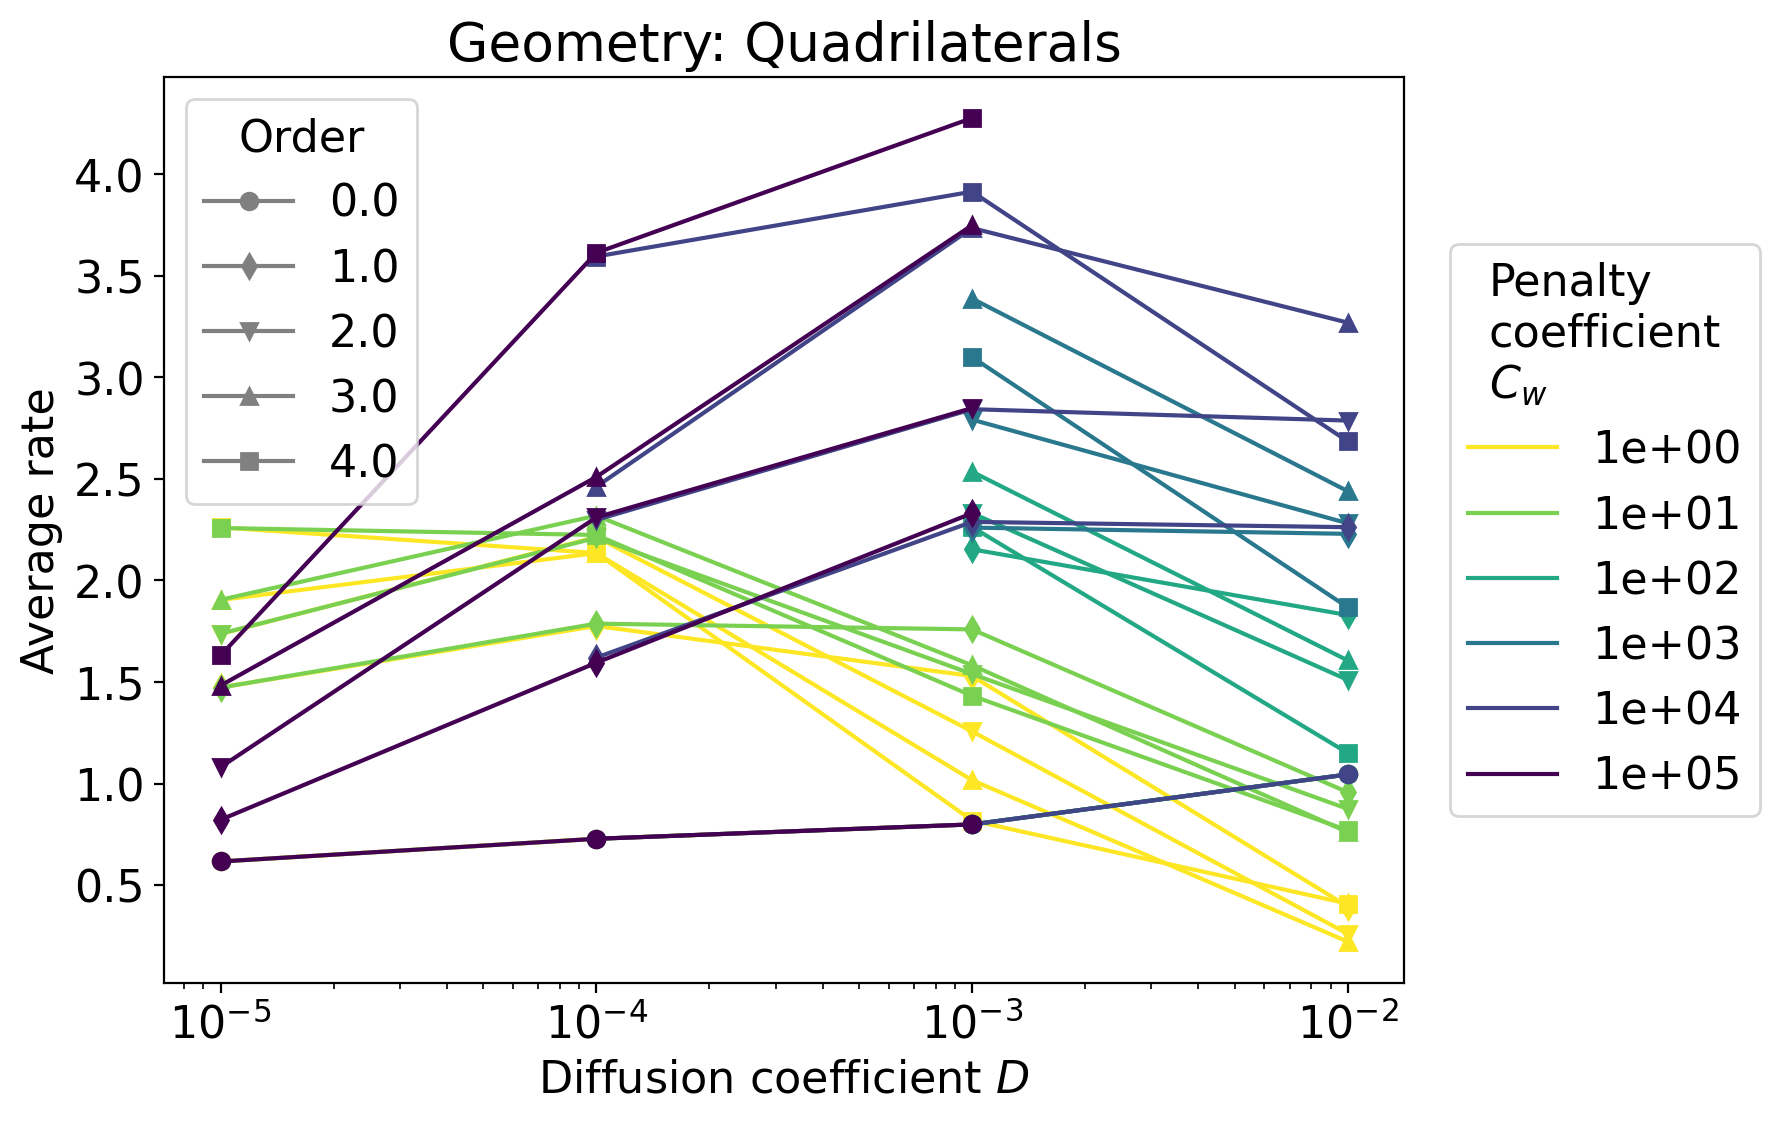
\includegraphics[width=0.49\textwidth]{../figs/parametric/advdiff_2D/ord_quarteroni2_2_4}
	&
	\vspace{0pt} 
	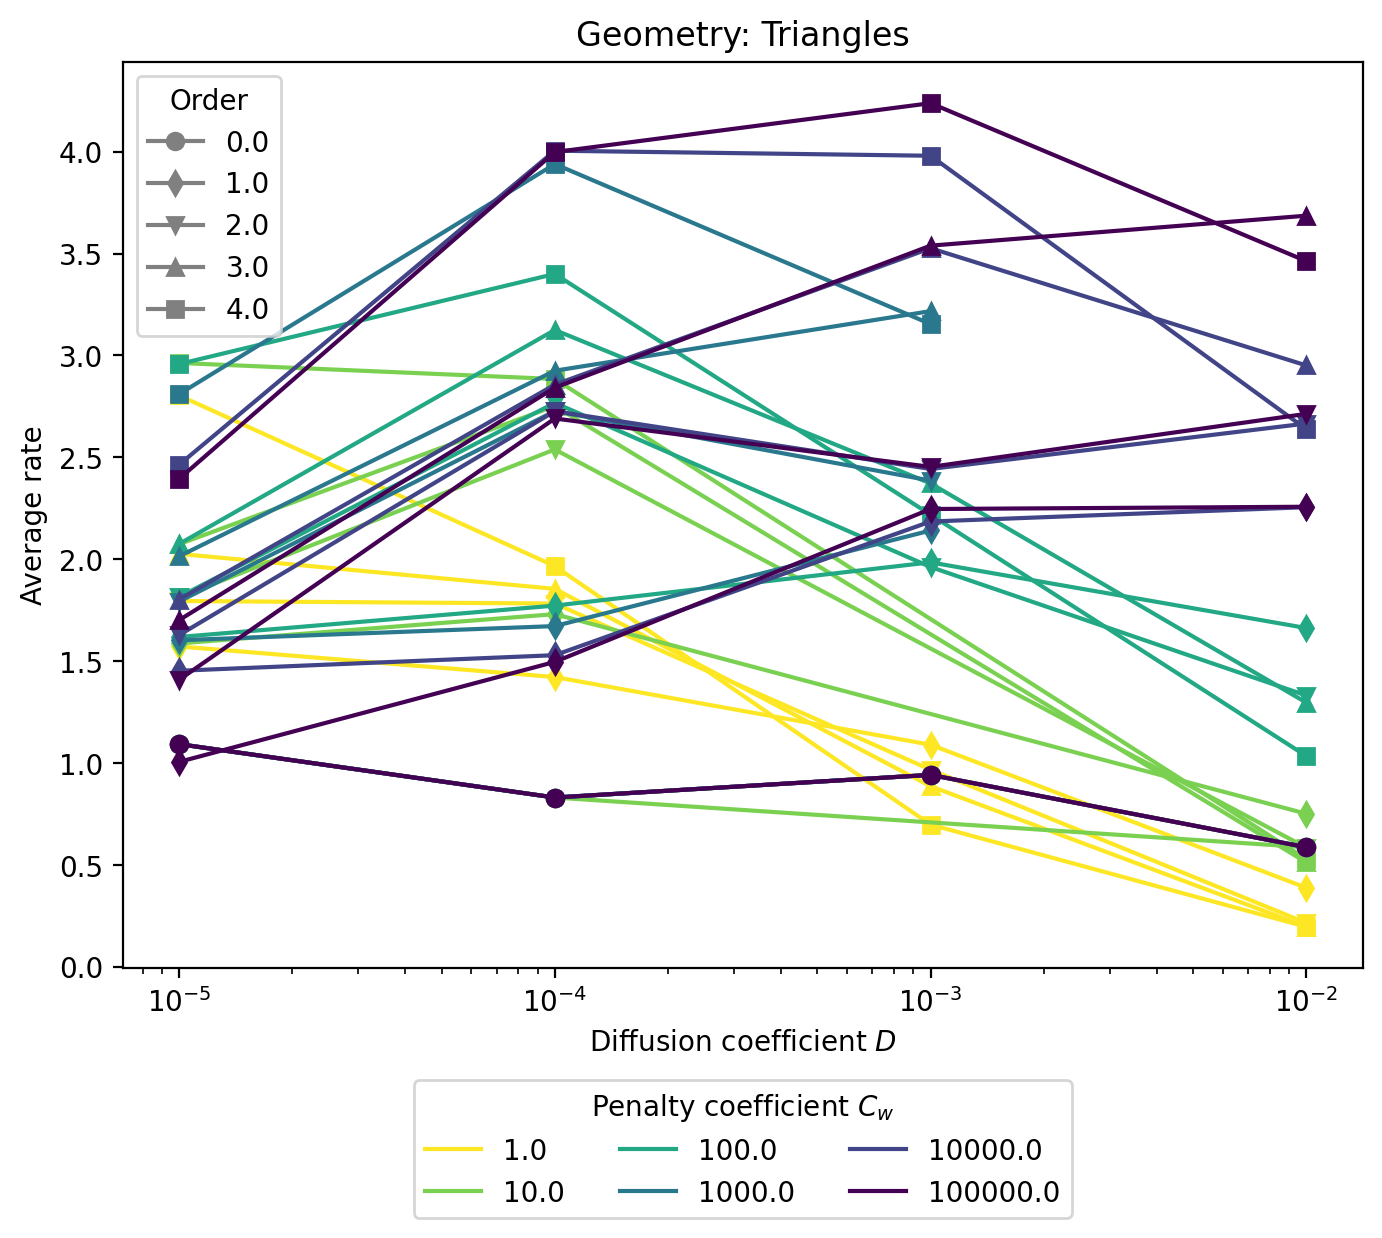
\includegraphics[width=0.49\textwidth]{../figs/parametric/advdiff_2D/ord_quarteroni2_2_3}
	\end{tabular}
	\caption{\Cref{ex:quart3} average order for different choice of $C_w$}
	\label{fig:orders_quarteroni3}
\end{figure}


\begin{figure}[p!]
	\centering
	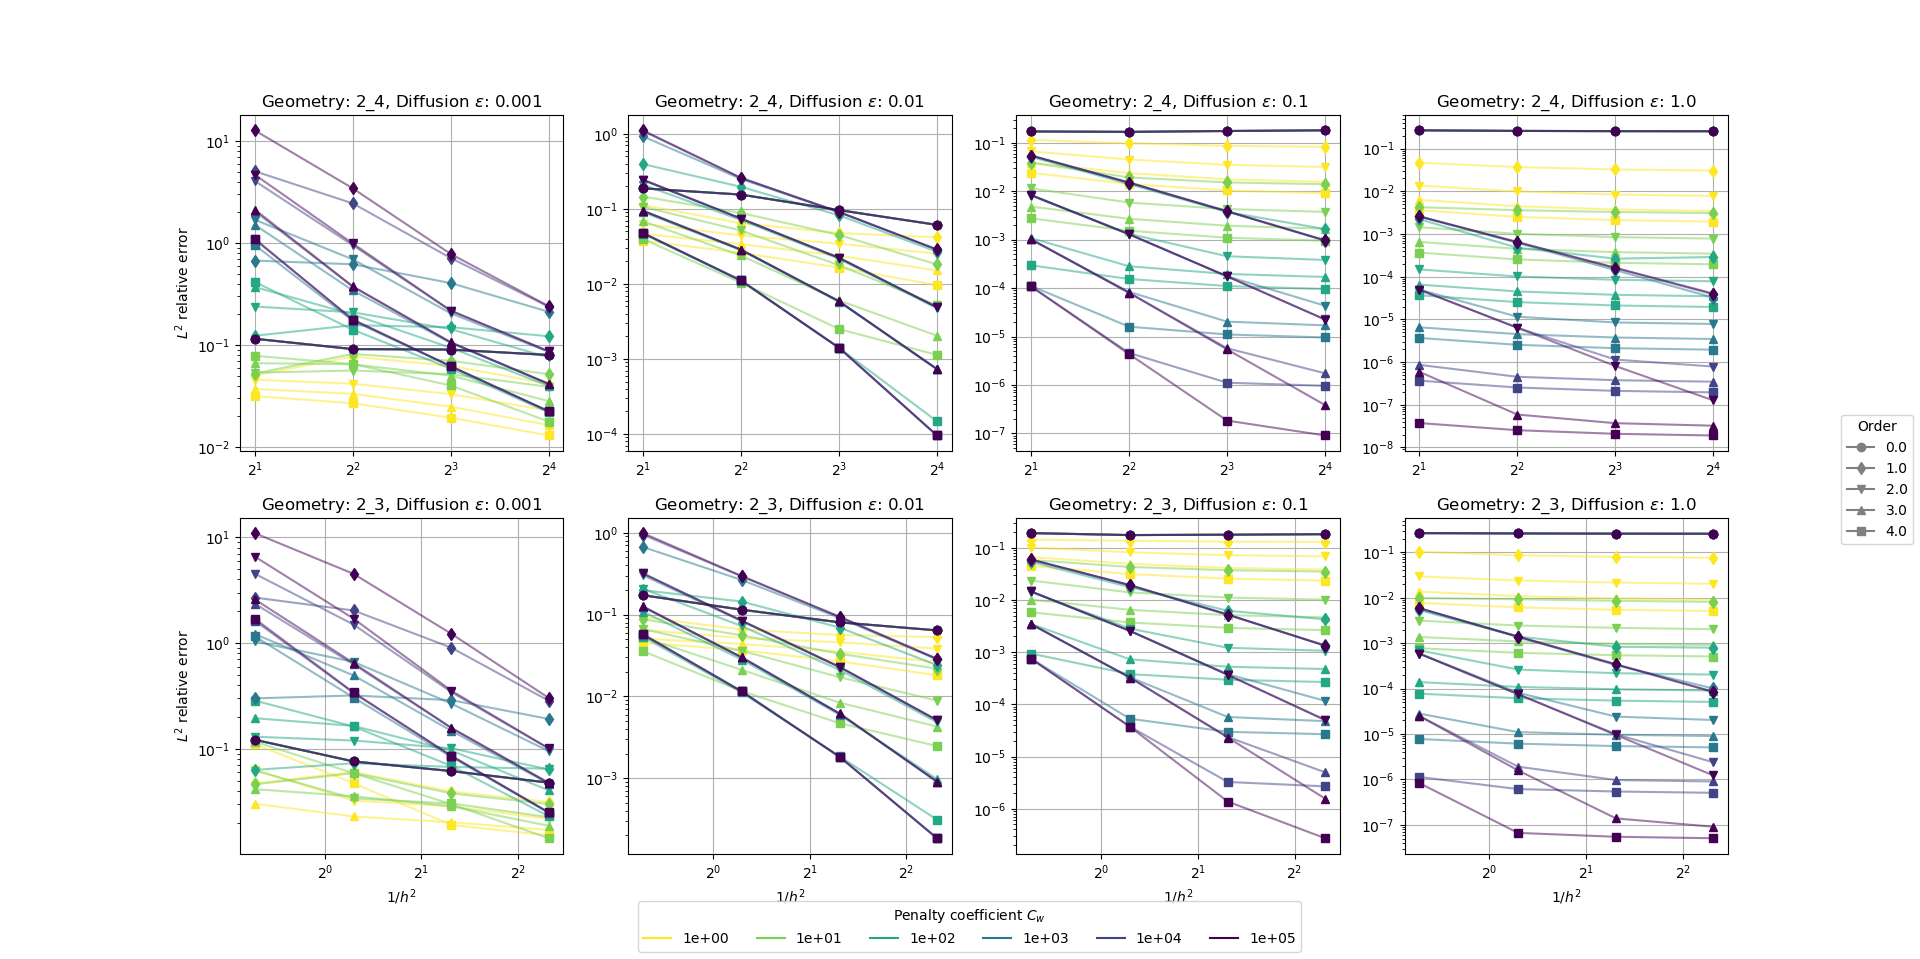
\includegraphics[height=\textheight]{../figs/parametric/advdiff_2D/quarteroni3.png}
	
	\caption{\Cref{ex:quart3} convergence graphs for different choice of $C_w$}
	\label{fig:conv_qart3}
\end{figure}

\newpage
\begin{example}[Viscous Burgers 1D]
\label{ex:burgers_hest}
Based on \cite[Section 7.1.2, Example 7.5,  p. 255]{Hesthaven2008}.
On $\Omega = [-1, 1]$ we will solve the viscous Burgers’ equation
\eqref{eq:ex_burgers} with the zero source function.
%\begin{equation}
%	\pdiff{u}{t} + \pdiff{}{x}\left(\frac{u^2}{2}\right) = D \pdiff{^2u}{x^2}
%\end{equation}
%where $D$ is diffusion coefficient.
This equation has an exact solution of a traveling wave
\begin{equation}
	u_{exact} =  -\tanh\left(-\frac{2 \, t - 2 \, x - 1}{4 \,D}\right) + 1.
\end{equation}
We set boundary conditions to match the solution
\begin{equation}
	\begin{aligned}
	& u(-1, t) = -\tanh\left(-\frac{2 \, t  + 1}{4 \,D}\right) + 1,
	&  u(-1, t) = -\tanh\left(-\frac{2 \, t - 3}{4 \,D}\right) + 1,\\
	&u_x(-1, t) = \frac{1}{2D}\tanh\left(-\frac{2 \, t + 1}{4 \, D}\right)^{2} -
	\frac{1}{2D},
	&u_x(1, t) = \frac{1}{2D}\tanh\left(-\frac{2 \, t - 3}{4 \, D}\right)^{2} -
	\frac{1}{2D}.
	\end{aligned}
\end{equation}
We will study the solution at time $t = 1$ with $D = 0.001$ and $D = 0.01$. The exact
solution is shown in \Cref{fig:burgers_hesthaven_ext}.
\begin{figure}[h]
	\centering
%	\begin{tabular}{p{0.5\textwidth} p{0.5\textwidth}}
%		\vspace{0pt}
%		\includegraphics[width=0.4\textwidth]{../figs/burgess_hesthaven_exact_t1_e001.png}
%		&
%		\vspace{0pt}
%		\includegraphics[width=0.4\textwidth]{../figs/burgess_hesthaven_exact_t1_e01.png}
%	\end{tabular}
%
	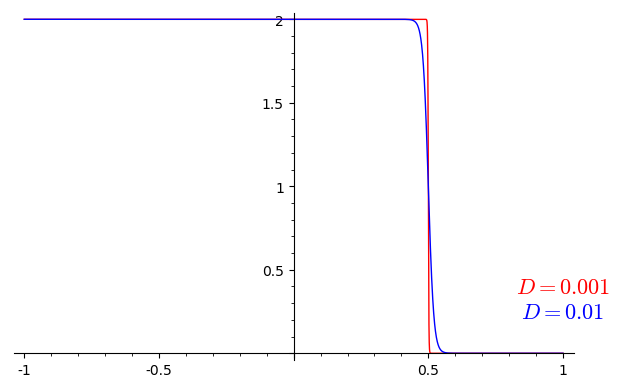
\includegraphics[scale=0.45]{../figs/burgers_hesthaven_exact_t1.png}
	\caption{\Cref{ex:burgers_hest}. Exact solution at $t = 1$.}
	\label{fig:burgers_hesthaven_ext}
\end{figure}
Different values of the coefficient $C_w$ in the penalty term yield different convergence
behavior as demonstrated in \Cref{fig:burgers_conv}. In this case increasing $C_w$ is detrimental to the accuracy of the solution for $D=0.001$ as it
develops into a steep step, see \Cref{fig:burgers_hesthaven_ext}, whose approximation
requires discontinuity in the approximate solution. For $D=0.01$ the diffusion leads to a much
more gradual solution and the penalty term counteracting discontinuity between elements
is beneficial, it also helps to counteract oscillations similarly to the limiter in
\Cref{ex:adv1D}. \todo Figure \ref{fig:burgers_sol} demonstrates where the errors come 
from.

\begin{figure}[h!]
    \centering
    \begin{subfigure}{.5\textwidth}
        \centering
        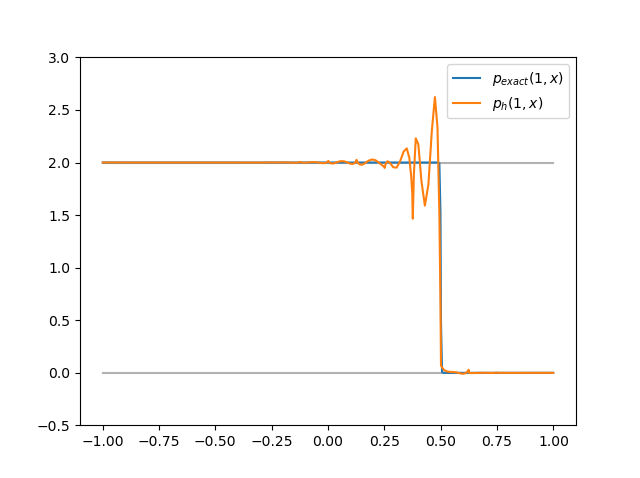
\includegraphics[width=\linewidth]{../figs/sols/burg1D-0002000100000-sol-h4o4}
        \caption{Limit: False}
    \end{subfigure}%
    \begin{subfigure}{.5\textwidth}
        \centering
        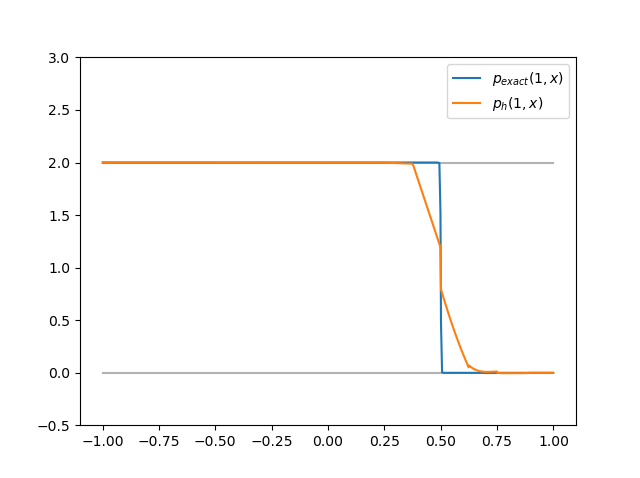
\includegraphics[width=\linewidth]{../figs/sols/burg1D-0002000000000-sol-h4o4}
        \caption{Limit: True}
    \end{subfigure}
    \caption{\Cref{ex:burgers_hest}. 4th order solution for $D=0.001$ with and without
        limiting.}
    \label{fig:burgers_sol}
\end{figure}

\end{example}

%\begin{figure}[h!]
%	\centering
%	\begin{tabular}{p{0.5\textwidth} p{0.5\textwidth}}
%		\vspace{0pt}
%
%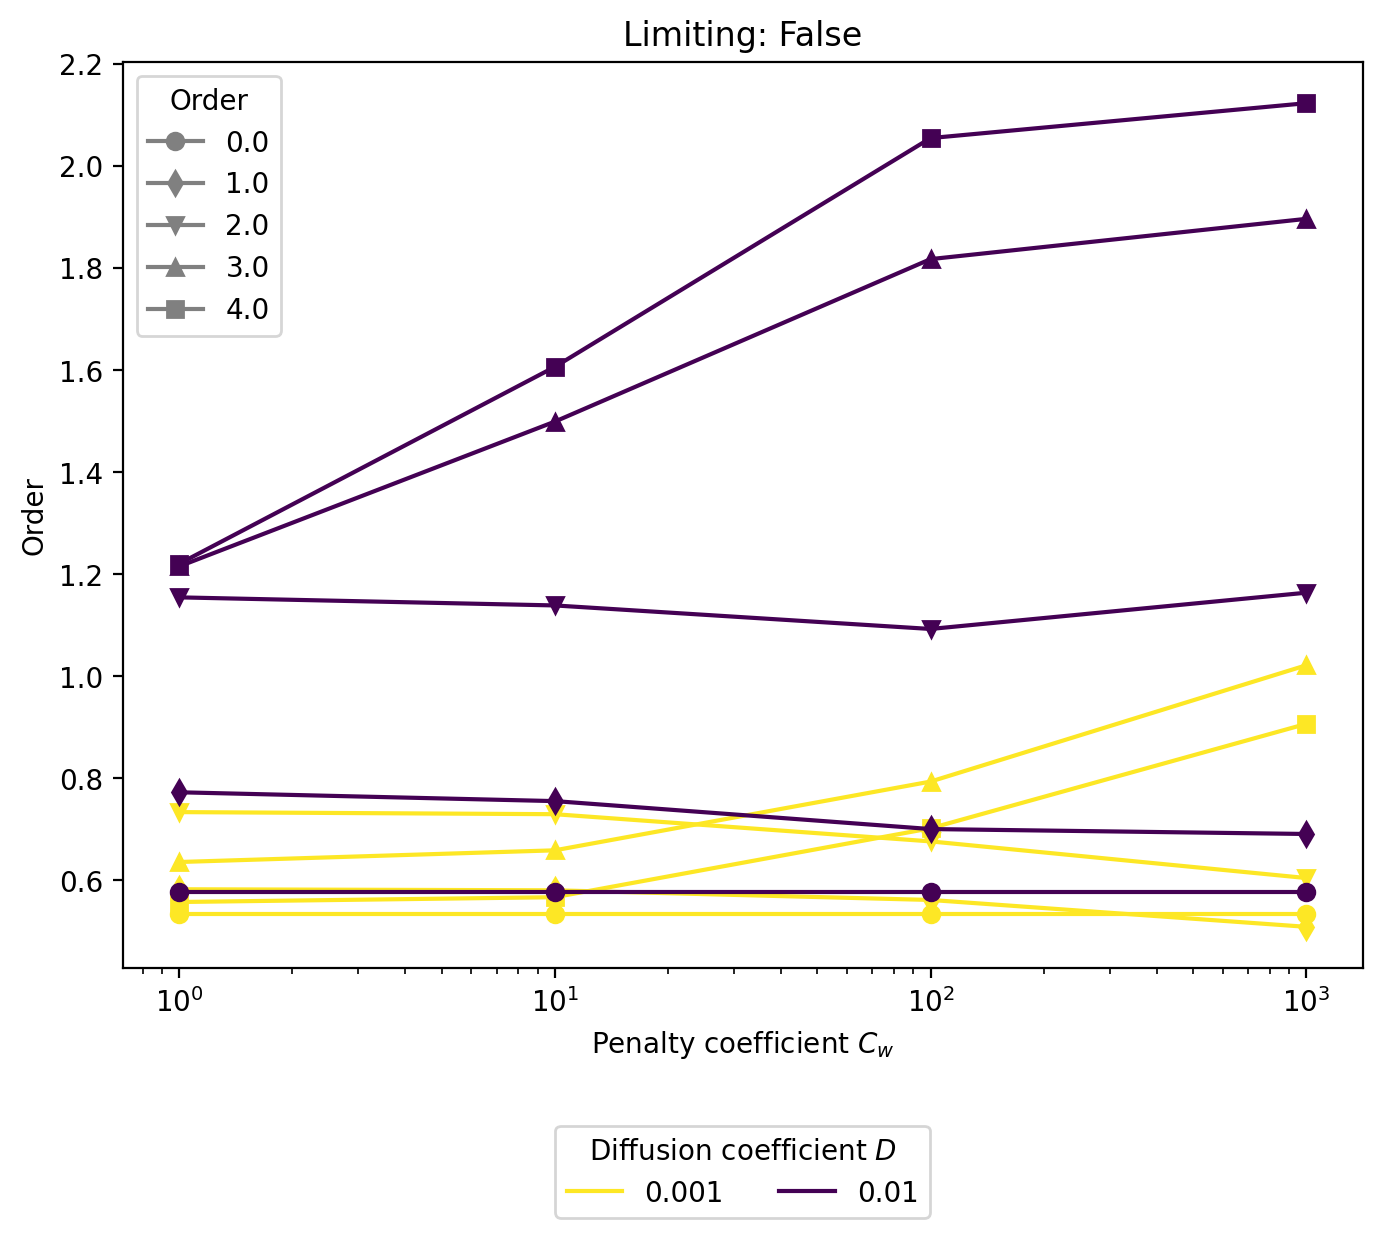
\includegraphics[width=0.49\textwidth]{../figs/parametric/burgers_1D/orders_unlimited}
%		&
%		\vspace{0pt}
%
%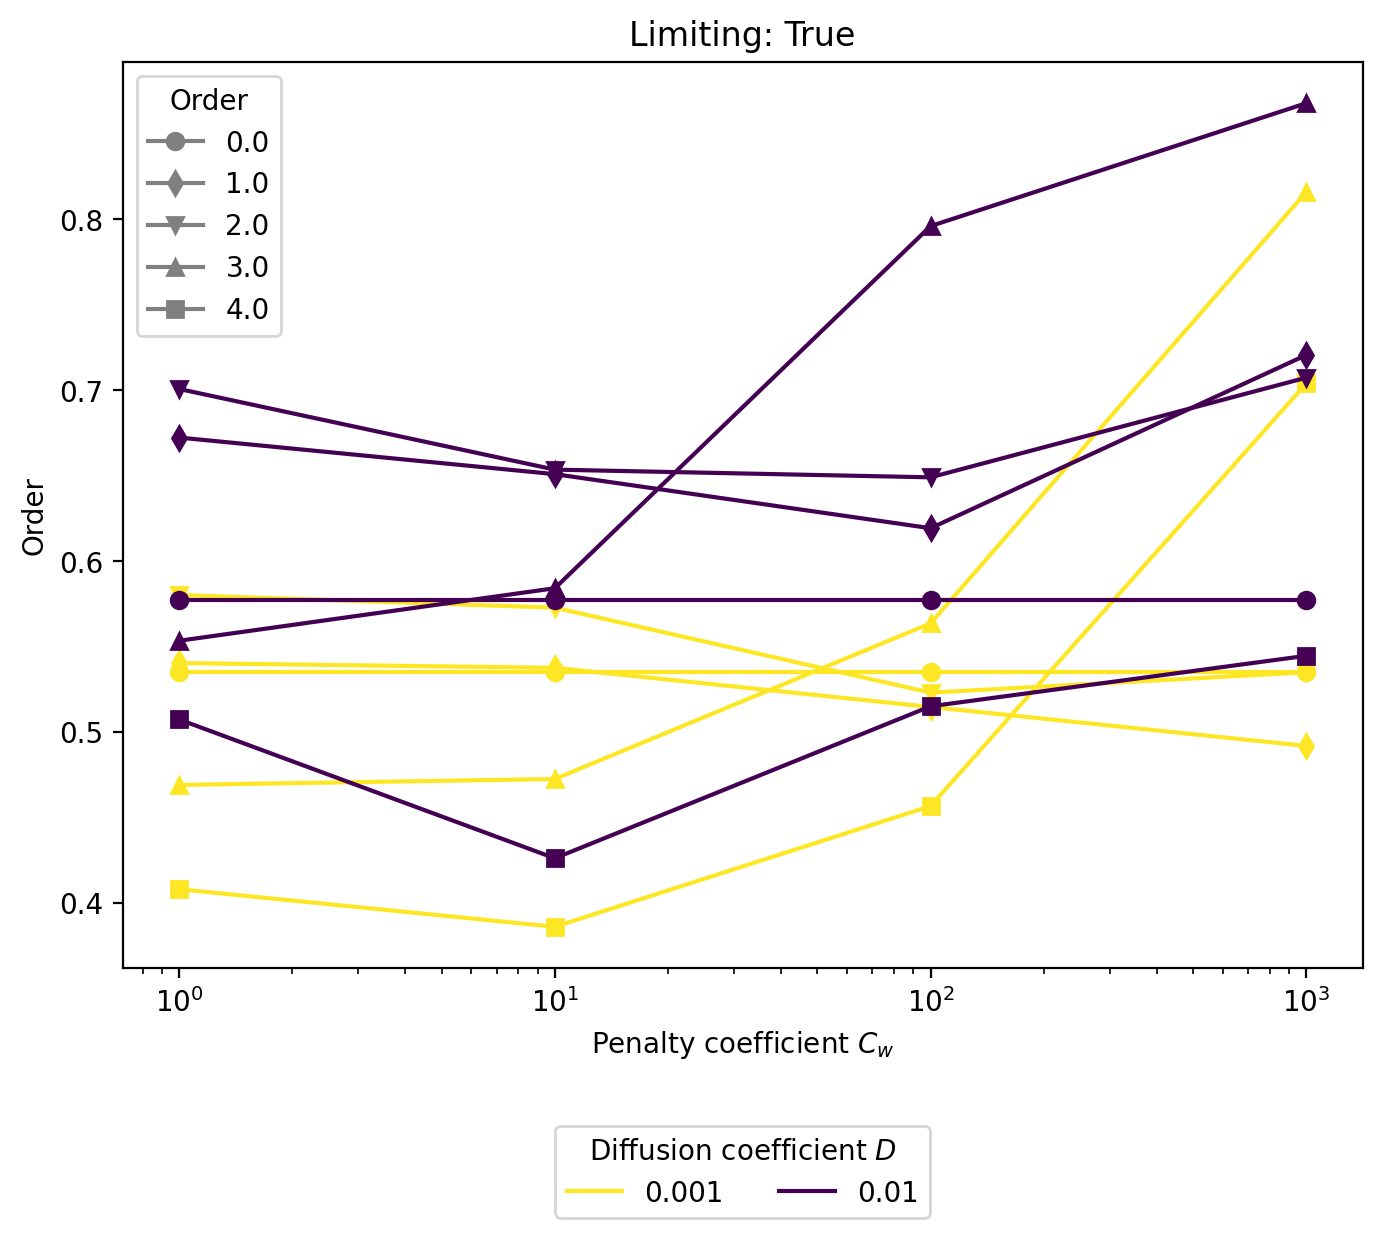
\includegraphics[width=0.49\textwidth]{../figs/parametric/burgers_1D/orders_limited}
%	\end{tabular}
%	\caption{\Cref{ex:burgers_hest} average convergence rates for different choices of
%	$C_w$}
%	\label{fig:burgess_orders}
%\end{figure}

\begin{figure}[p!]
	\centering
	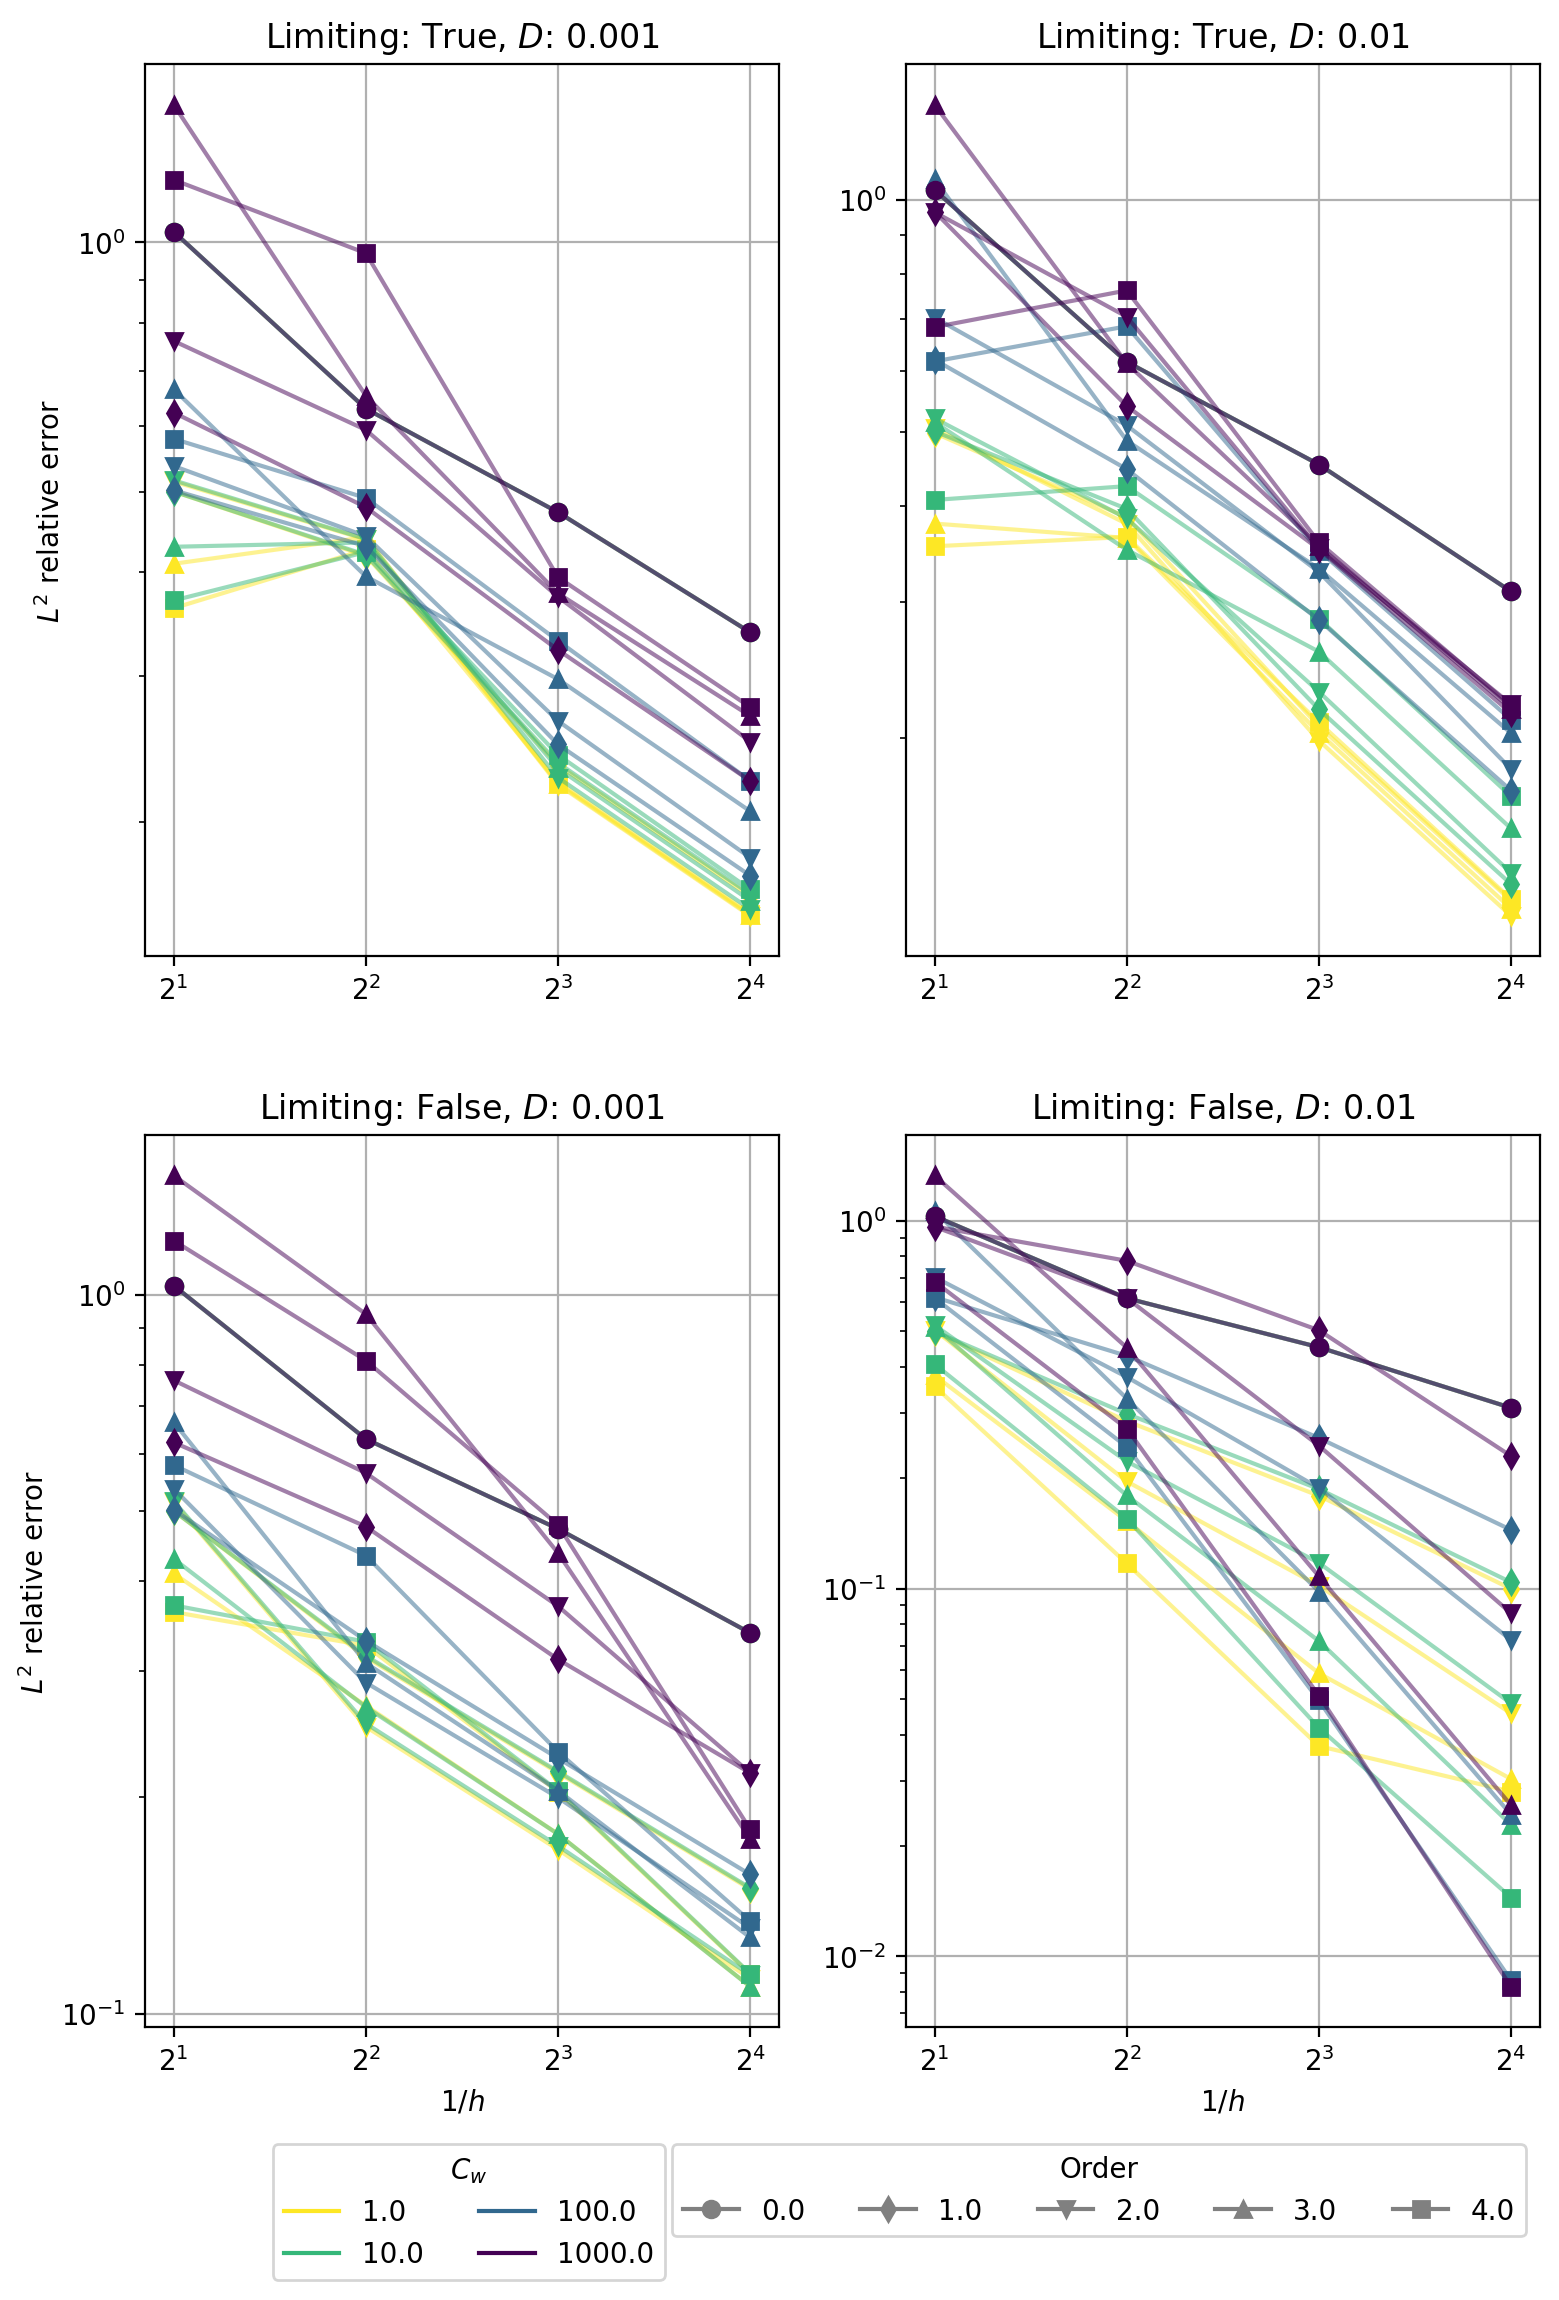
\includegraphics[width=\textwidth]{../figs/parametric/burgers_1D/convergences}
	\caption{\Cref{ex:burgers_hest}. Relative errors for different choices of $C_w$}
	\label{fig:burgers_conv}
\end{figure}
\clearpage

%\begin{figure}
%	\centering
%	\includegraphics[width=\textwidth]{../figs/err-sols/burgess_hesthaven-err-sol-i20cw1_d001_t2}
%	\includegraphics[width=\textwidth]{../figs/err-sols/burgess_hesthaven-err-sol-i20cw10_d001_t2}
%	\caption{Example 9 Exact solution (gray), numerical solution (orange) and their absolute difference (red) for
%	different orders and $h$. The left $y$ axes correspond to the solutions, the right ones to their difference.}
%	\label{fig:err_sol_burges_hest}
%\end{figure}

\newpage
\begin{example}[Viscous Burgers 2D]
\label{ex:kucera}
Based on example in \cite[Section 1.6]{Kucera},
we will solve equation \eqref{eq:ex_burgers} in $\Omega = \langle 0, 1 \rangle^2$.
%\begin{equation}
%		\pdiff{u}{t} + \frac{1}{2}\left(\pdiff{u^2}{x} + \pdiff{u^2}{y}\right)  - 
%		D \cdot \left( \pdiff{^2 u}{x^2} + \pdiff{^2 u}{y^2} \right) 
%		= g
%\end{equation}
%where $D$ is diffusion coefficient and $g$ is a source function. 
We setup boundary condition and source function in such way that the exact 
solution $u_{exact}$ is
\begin{equation}
	u_{exact} =  \ -{\left(e^{\left(-t\right)} - 1\right)} {\left(\sin\left(5 \,x 
	y\right) + \sin\left(-4 \, 
	x y + 4 \,x + 4 \, y\right)\right)}.
\end{equation}
We omit analytical forms of $g$ and boundary conditions for brevity.
Different values of coefficient $C_w$ in penalty term then yield only slightly different 
convergence behavior as demonstrated in Figure \ref{fig:kucera_conv} and 
\Cref{fig:kucera_orders}. In this case the solution does not feature any sharp steps and 
increase in penalty coefficient leads to increase in accuracy. In \Cref{fig:sol_kucera} 
this effect is clearly visible in sample solution, similarly to \Cref{ex:quart1}. Kučera 
in \cite{Kucera} reports average convergence rates for irregular triangular mesh 
slightly higher then ours.

\end{example}
\begin{figure}[h!]
	\centering
	\begin{tabular}{p{0.5\textwidth} p{0.5\textwidth}}
		\vspace{0pt} 
		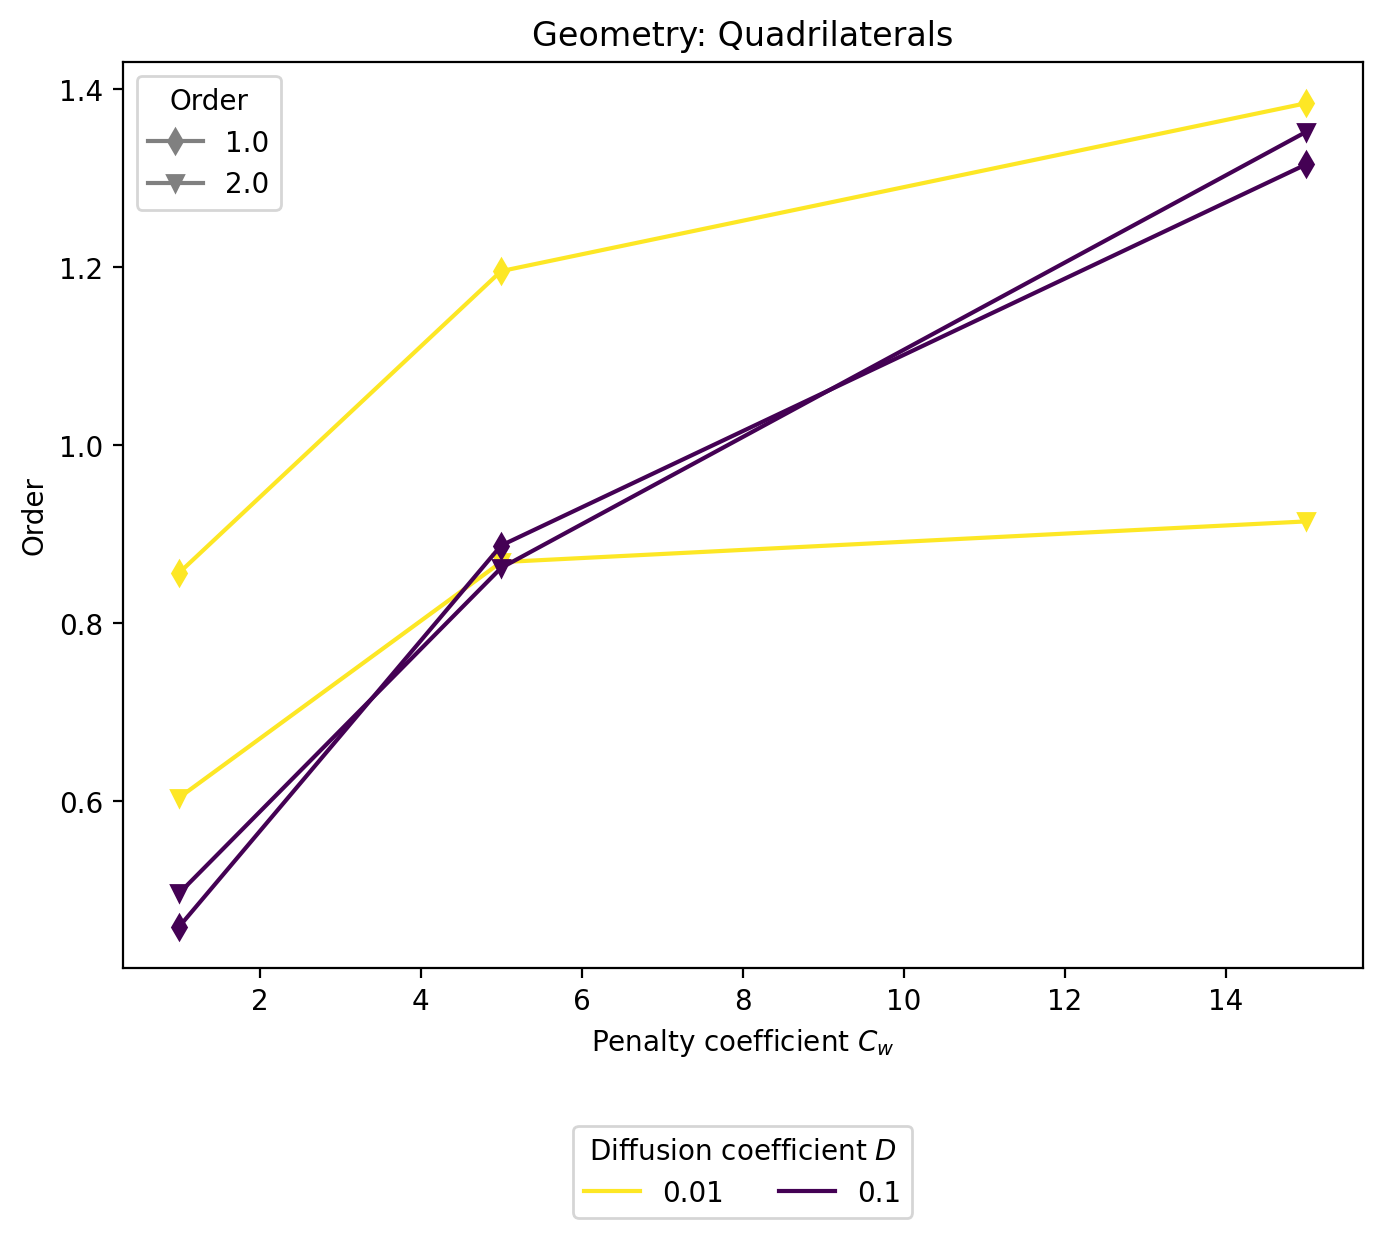
\includegraphics[width=0.49\textwidth]{../figs/parametric/burgers_2D/orders_2_4}
		&
		\vspace{0pt} 
		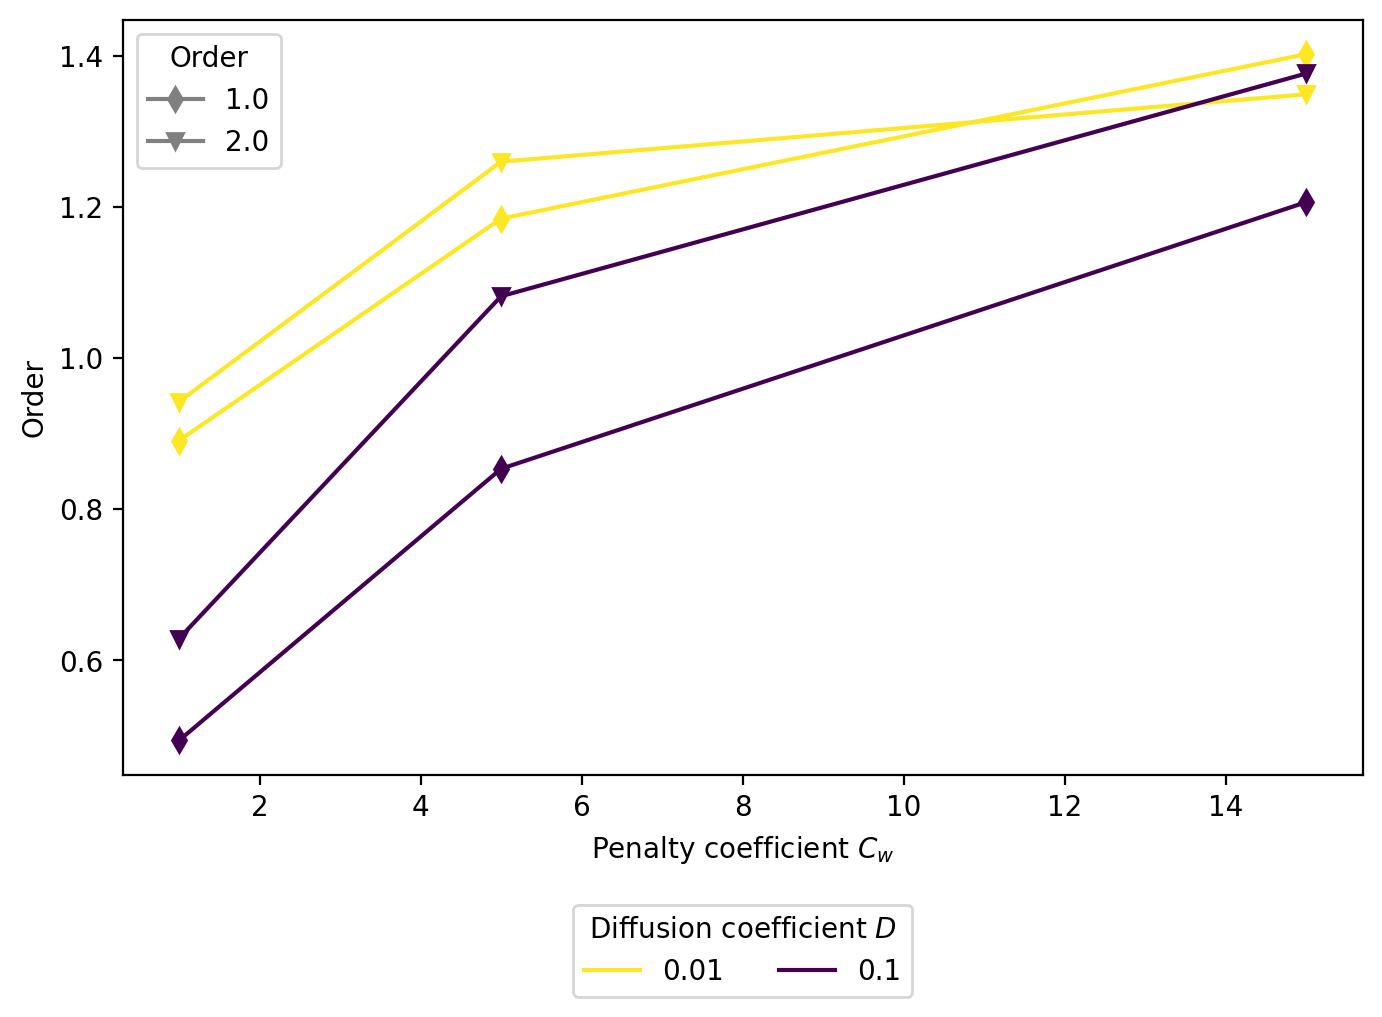
\includegraphics[width=0.49\textwidth]{../figs/parametric/burgers_2D/orders_2_3}
	\end{tabular}
	\caption{\Cref{ex:kucera}. Average orders for different values of $C_w$ for 
	quadrilaterals (left) and triangles (right).}
	\label{fig:kucera_orders}
\end{figure}


\begin{figure}[h!]
	\centering
	\begin{subfigure}{.5\textwidth}	
		\centering	
		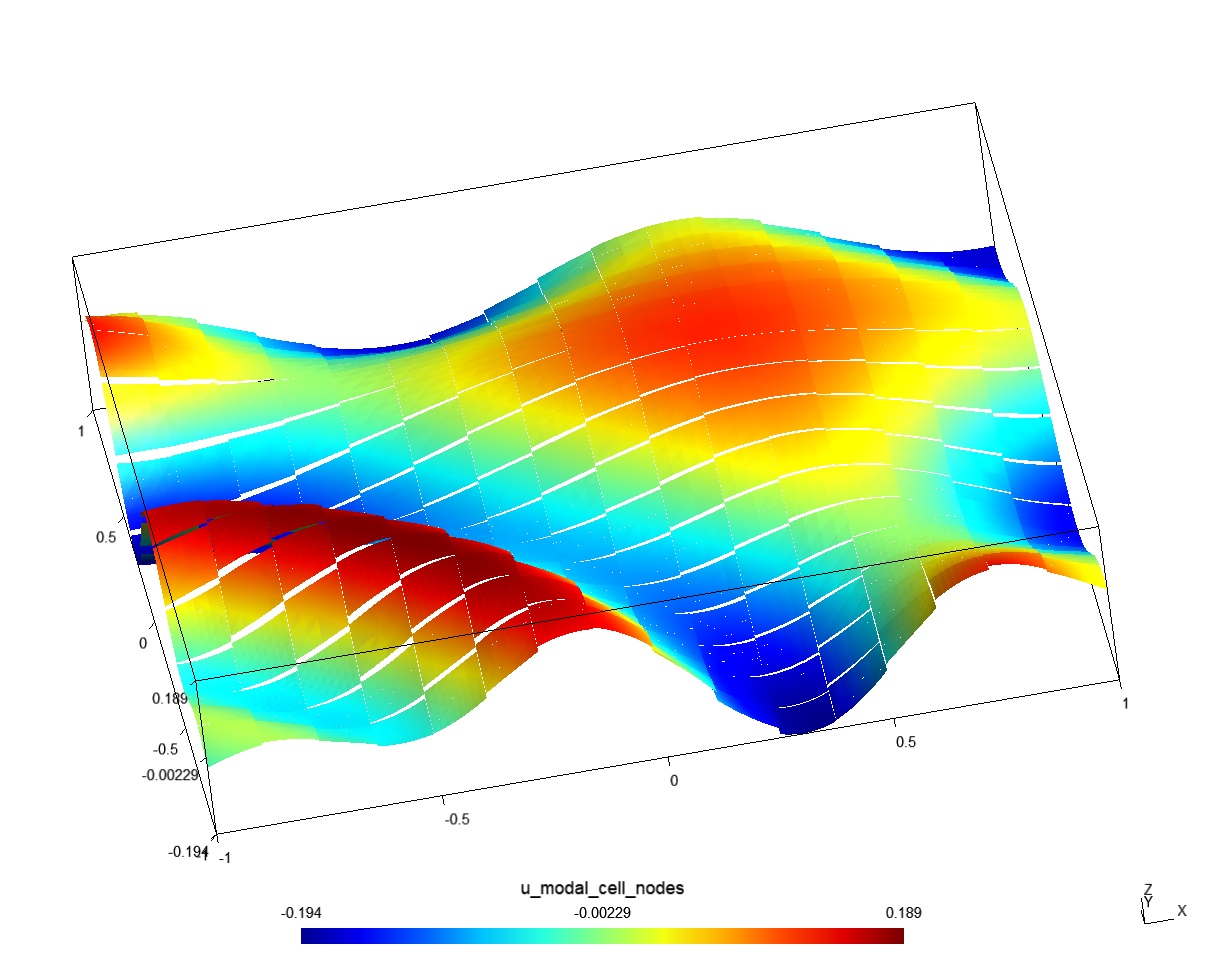
\includegraphics[width=\linewidth]{../figs/sols/kucera-010000000-sol-h256o02}
		\caption{$C_w = 1$}
	\end{subfigure}%
	\begin{subfigure}{.5\textwidth}
		\centering	
		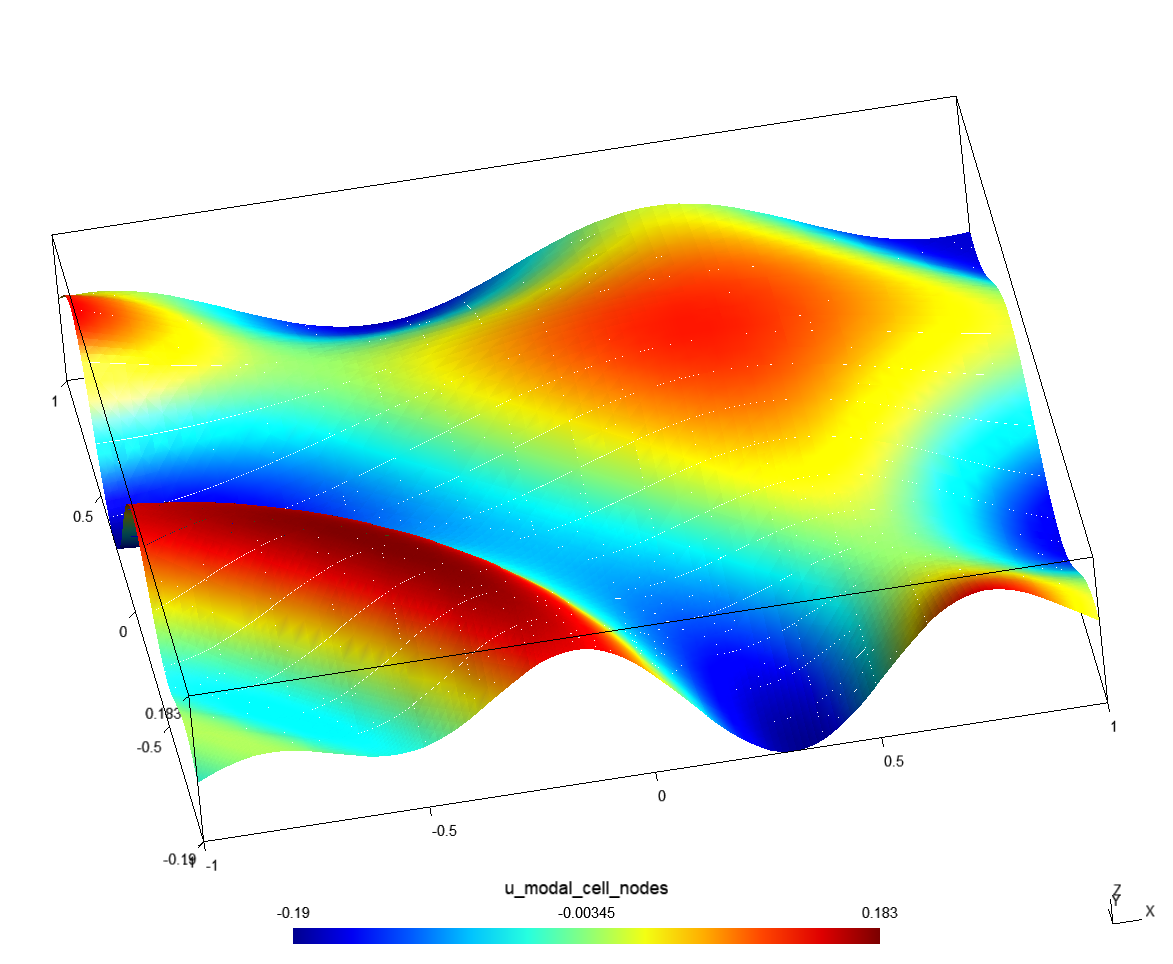
\includegraphics[width=\linewidth]{../figs/sols/kucera-212000000-sol-h256o02}
		\caption{$C_w = 15$}
	\end{subfigure}
	\caption{\Cref{ex:kucera}. Solution for different values of $C_w$ on a quadrilateral 
	mesh.}
	\label{fig:sol_kucera}
\end{figure}

\begin{figure}[p!]
	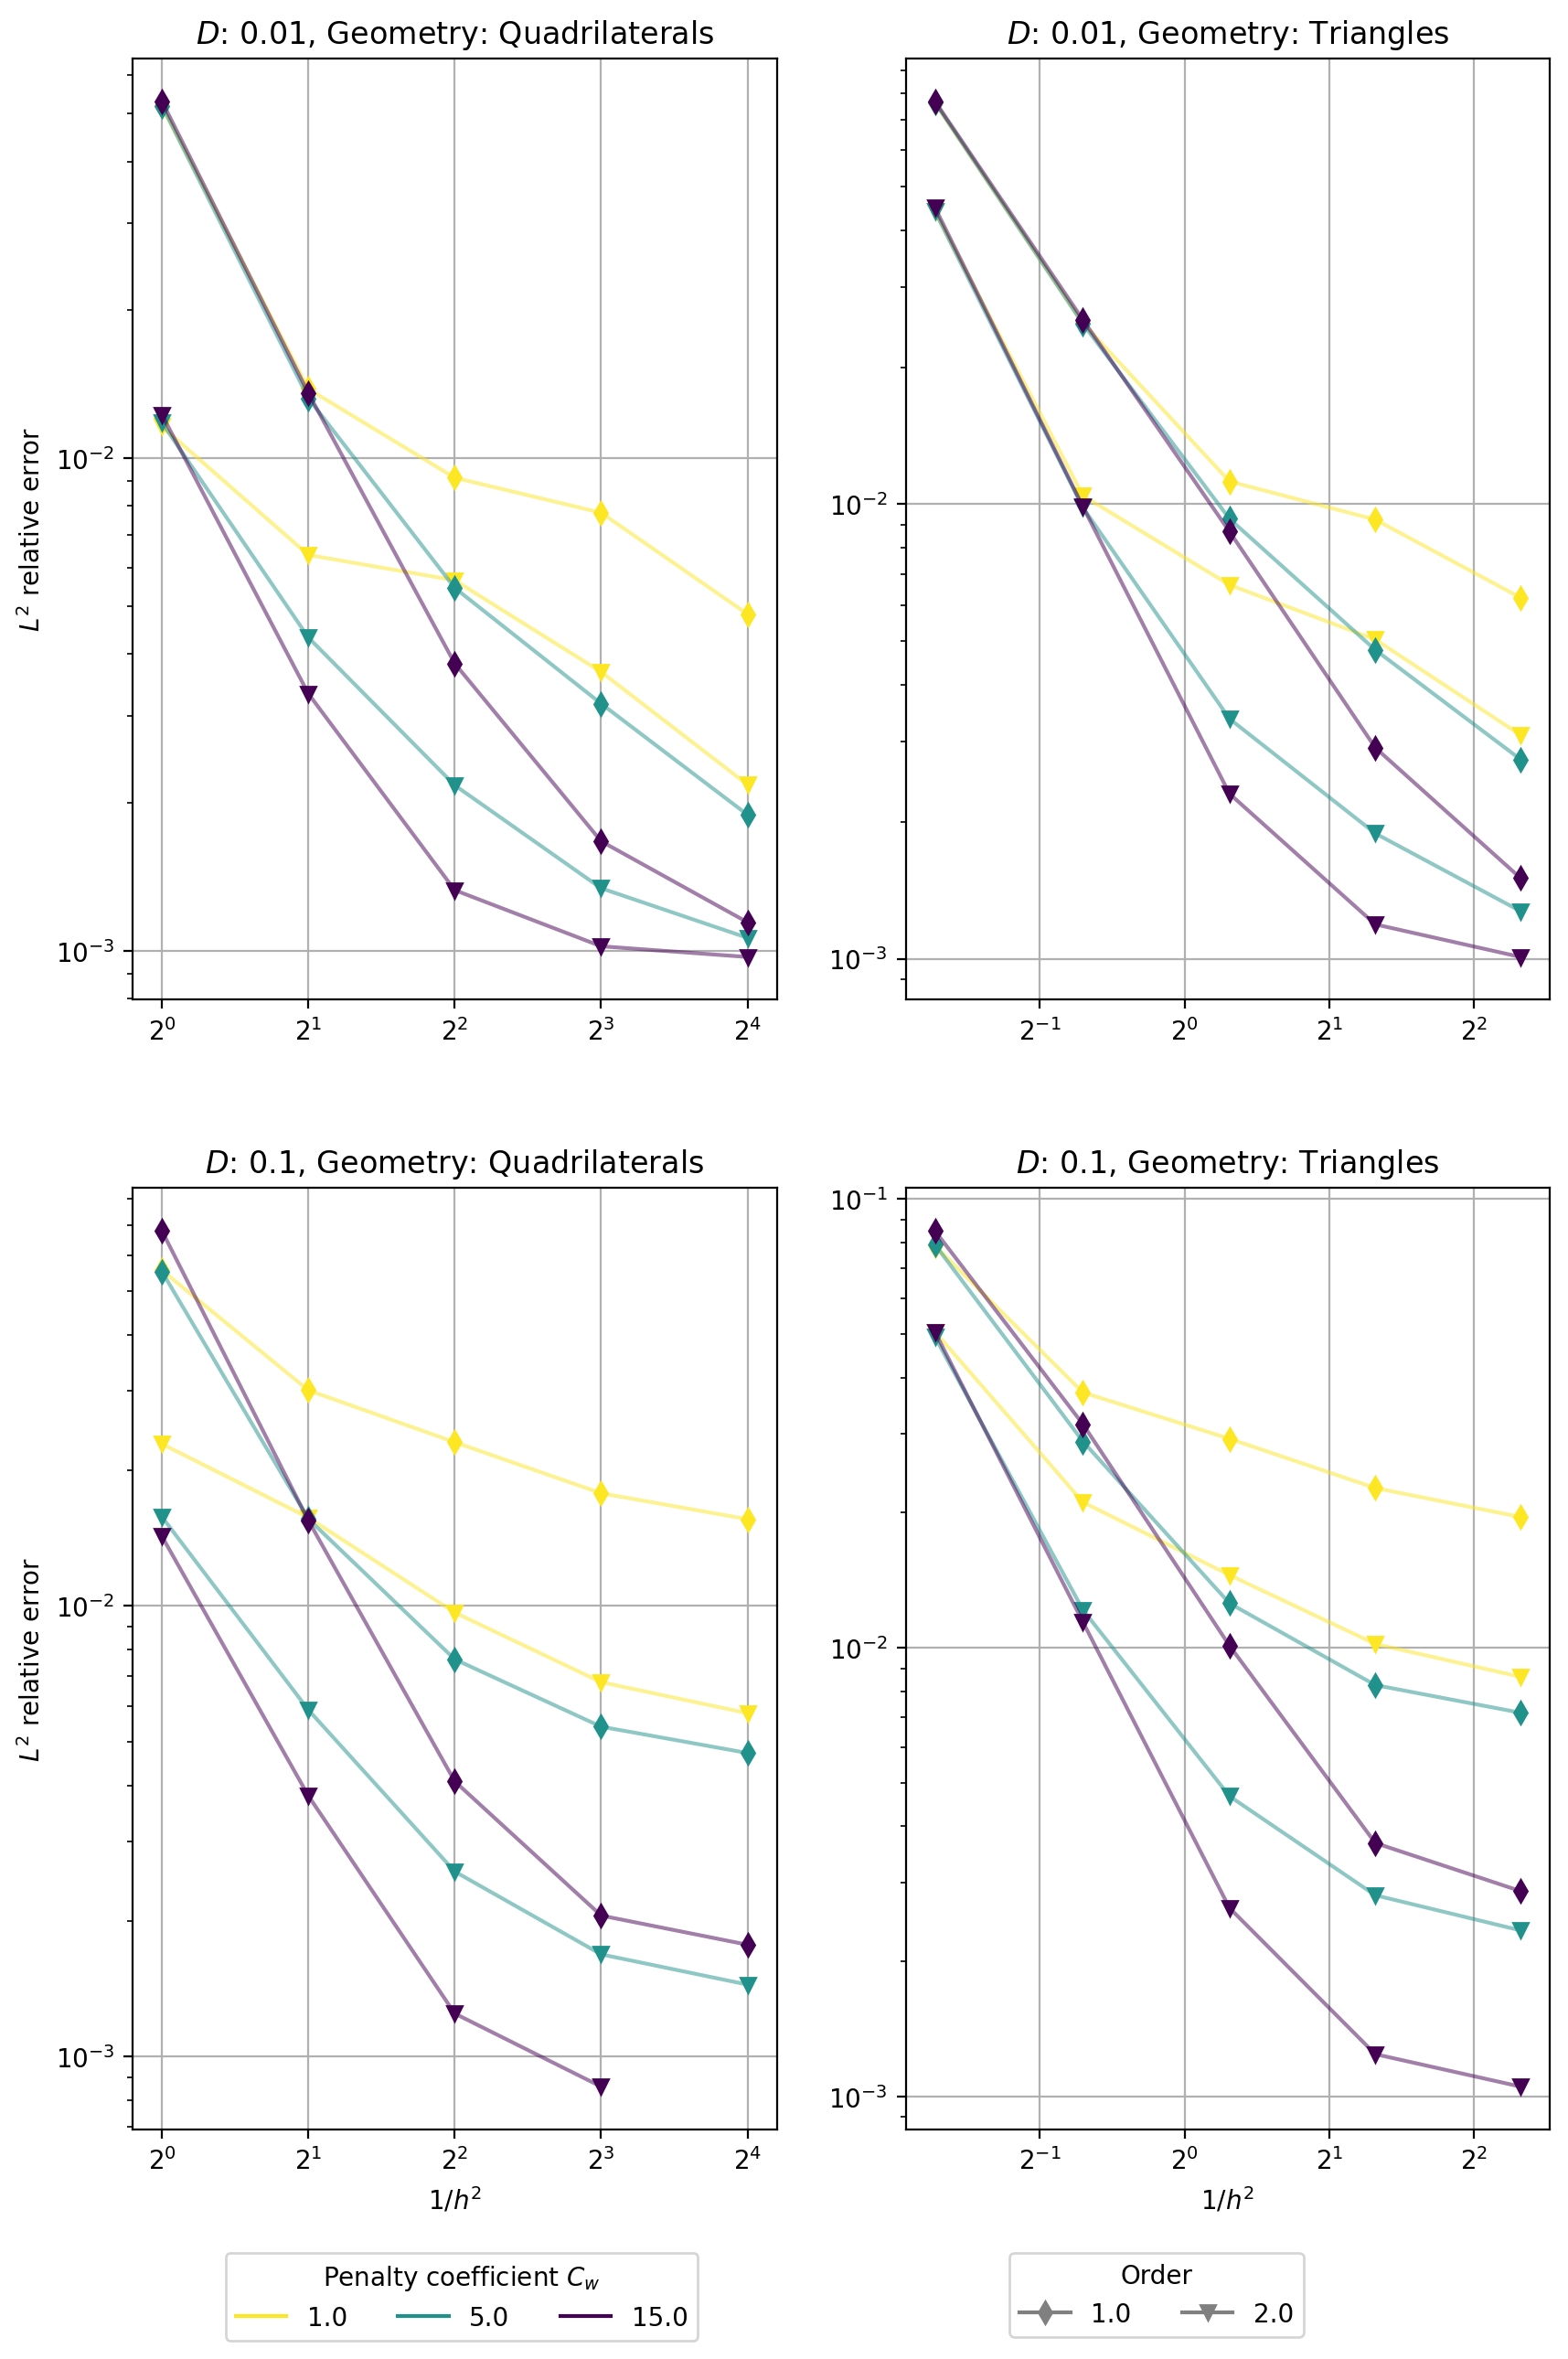
\includegraphics[width=\textwidth]{../figs/parametric/burgers_2D/convergence_symmetry}
	\caption{\Cref{ex:kucera}. Relative errors for different choices of $C_w$ for 
	quadrilaterals (left) and triangles (right).}
	\label{fig:kucera_conv}
\end{figure}

\chapter{Conclusion}
\label{ch:conclusion}
% !TeX spellcheck = en_US
%%
%% Text of diploma thesis
%%
%% Tomáš Zítka
%%
\paragraph{Implementation}
In this work we implemented discontinuous Galerkin method into SfePy package. SfePy uses 
term based syntax for building discretizations of equations, we implemented several 
new terms, namely linear advection flux term, general hyperbolic flux term, diffusion 
flux and diffusion penalty term, and general term for computing integral
$$
\int_{T^k} \vec{f}(P_i^k\psi_i)\cdot\nabla\psi_j. 
$$
Along with wide range of terms already present in SfePy this allows users to discretize 
variety of useful equations. To enable solving transient equations we implemented two 
explicit time stepping solvers, forward Euler and TVD Runge-Kutta of 3rd order 
solver. Moreover we implemented moment limiters for 1D and 2D transient problems.

\paragraph{Analysis}
To study properties of the method we measured convergence rates for seven example 
problems chosen from literature. For some of them we present results to our knowledge not 
available in literature. For transient problems the performance of the method is hindered 
by used time stepping solvers, nevertheless the method still performs to the expectations.
[\todo more on examples when they are finished]

\paragraph{Possible improvements and suggestions for further work}
Although from the time and memory requirements perspective the implementation of the 
method scales well enough with SfePy capabilities, there is still room for improvement. 
Calls of \pysauce{numpy.einsum} could use optimized tensor contraction path, which could 
be retained between individual term evaluation (i.e. between time steps). 
The implementation of limiters is rather ad-hoc and refactoring it to bring it in line 
with design of other SfePy elements would help making code more readable and their usage 
simpler and more versatile. 

One important feature available in SfePy missing from this DG FEM implementation is 
ability to solve systems of PDEs. This lack could inspire future work as it would 
requires substantial modification of flux terms as well as implementation of  
strategies for evolving systems of interest like Euler or Navier-Stokes equations. 
Further besides implemented Lax-Friedrichs flux there is variety of other fluxes for 
examples Godunov flux or some problem specific fluxes like [\todo cite] designed 
specifically for solving Euler equation Thanks to versatility of problem specification 
this would also unlock large potential for further study of the method behavior. 

\begin{itemize}
	\item Godunov and other fluxes
\end{itemize}



\section*{Acknowledgment}
 DPP v rámci řešení projektu GACR 16-03823S

%\section{Doc test}
%\begin{equation}
%	C = \max_{p \in [1, 2]}\left\lvert n_x \frac{\partial p}{\partial a_1} +
%	n_y\frac{\partial p}{\partial a_2} \right\rvert =
%	\max_{p \in [1, 2]} \left\lvert  \ul{n} \cdot \nabla p \cdot \ul{a} \right\rvert
%\end{equation}

% TODO resolve citation format
%\nocite{*}

\addcontentsline{toc}{chapter}{Bibliography}
\bibliographystyle{plain}
\bibliography{dg_fem_literature}


%\glsaddall % list all
%\renewcommand*{\acronymname}{Seznam použitých zkratek}
%\addcontentsline{toc}{chapter}{Seznam použitých zkratek}
%\printnoidxglossaries % print acronym without having to call indexer(?)
\addtocontents{toc}{\protect\enlargethispage{2\baselineskip}}
\begin{appendix}
	

	
\end{appendix}


\end{document}